\subsection{Inclusive ZZ cross section measurement}

The inclusive cross-section is determined as 
$$\sigma_{pp\to ZZ} = \frac{N_{data}-N_{bkg}}{\mathcal{L}\cdot A \cdot \epsilon \cdot \mathcal{B}(Z\to \ell^+\ell^-)\cdot\mathcal{B}(Z\to \ell'^+\ell'^-)},$$
where $N_{data}$ and $N_{bkg}$ are the total number of data and background events, $A$ is the geometrical acceptance, $\epsilon$ is the signal efficiency, $\mathcal{L} = 19.7$ fb$^{-1}$ is the integrated luminosity and $\mathcal{B}(Z\to \ell^+\ell^-) = 3.363 \pm 0.004$ ($3.366\pm 0.007$)\% is the branching fraction of a $Z$ boson decaying into an electron (muon) pair~\cite{PDG}.

The region in which the measurement is performed (called ``fiducial region'') is defined by requiring the invariant mass of each Z boson 
between 60 and 120 GeV. % and the invariant mass of the Z-boson pair ($m_{ZZ}$) above 100 GeV. 
The product of acceptance and efficiency ($A\cdot\epsilon$) is evaluated from simulation and defined as the ratio between the
number of events in the fiducial region that pass the analysis selection at reconstruction level and the number of events generated in that
fiducial region. 
%sum of $q\bar{q} \to ZZ$ and  $gg \to ZZ$ generated events, with $Z\to \ell^+\ell^-$, and the events accepted by the analysis
%selection at reconstructed level corrected for each individual lepton flavor in bins of pT and h using factors obtained with the ``tag-and-probe'' technique. 
The requirements on $p_T$ and $\eta$ for the particles in the final state reduce the full possible phase space of the $ZZ \to 4
\ell$ measurement by a factor within a range of 0.32-0.47 for the $4e$, $4\mu$ and $2e2\mu$ (depending on
the final state) with respect to all events generated in the mass window $60 < m_{Z_1} ,m_{Z_2} < 120$ GeV.
The $A\cdot\epsilon$ product estimated for each final state and for the different samples is listed in 
Tables~\ref{tab:Aeps_tot} and ~\ref{tab:Aeps_samples}.

%\begin{table*}[htbH]
%\begin{center}
%\caption{Selection efficiency and $A\cdot \epsilon$ product for the three final states used in the $pp\to ZZ$ cross-section measurement.
%%The values reported are a product of the detector geometrical acceptance and the object reconstruction and event identification efficiency.
%}
% \label{tab:Aeps_tot}
%\begin{tabular}{ccc}
%\hline Final State & $\epsilon$ & $A\cdot\epsilon$\\
%\hline $4\mu$ & 84\%& 47\%  \\
%$4e$ & 55\%& 32\%\\
%$2e2\mu$ &69\%& 40\%\\
%\hline
%\end{tabular}
%\end{center}
%\end{table*}

\begin{table*}[htbH]
\begin{center}
\topcaption{$A\cdot \epsilon$ for the three final states used in the $pp\to ZZ$ cross-section measurement.
The values reported are a product of the detector geometrical acceptance and
the object reconstruction and event identification efficiency. \label{tab:Aeps_tot}}
\begin{tabular}{cc}
\hline Final State & $A\cdot\epsilon$\\
\hline $4\mu$ & 47\%  \\
$4e$ & 32\%\\
$2e2\mu$ & 40\%\\
\hline
\end{tabular}
\end{center}
\end{table*}

\begin{table*}[htbH]
\begin{center}
\caption{Signal yield and efficiency for the signal samples.
The $A\cdot\epsilon$ values reported are a product of the detector geometrical acceptance and
the object reconstruction and event identification efficiency.}
 \label{tab:Aeps_samples}
\begin{tabular}{lcccccc}
\hline  \multicolumn{1}{c}{Process} & \multicolumn{3}{c}{Signal yield} & \multicolumn{3}{c}{$A\cdot\epsilon$}\\
\hline  & $2e2\mu$ & $4e$& $4\mu$ & $2e2\mu$ & $4e$ &$4\mu$\\ 
\hline $ZZ\to 4\ell$ (\texttt{MadGraph}) & 125.3& 51.7 &51.7 &0.39 & 0.32& 0.46  \\
 $q\bar{q}\to ZZ\to 4\mu$  (\texttt{Powheg})& - & - & 69.6 & - & - & 0.46\\
$q\bar{q}\to ZZ\to 4e$  (\texttt{Powheg}) & - & 48.0 & - & - & 0.32 & -\\
$q\bar{q} \to ZZ\to 2e2\mu$  (\texttt{Powheg}) & 117.6 & - & - & 0.39 & - & -\\
$gg\to ZZ\to 4\mu$  (\texttt{MCFM})& - & - & 5.04& - & - & 0.72\\
$gg\to ZZ\to 4e$  (\texttt{MCFM}) & - & 3.47 & - & - & 0.49 & -\\
$gg\to ZZ\to 2e2\mu$  (\texttt{MCFM})& 8.52 & - & - & 0.60 & - & -\\
$ZZ\to 4\mu +2jets$  (\texttt{Phantom})& - & - & 0.633 & - & - & 0.65\\
$ZZ\to 4e +2jets$  (\texttt{Phantom})& - & 0.440 & - & 0.45 &-\\
$ZZ\to 2e2\mu +2jets$  (\texttt{Phantom})& 1.08 & - & - & 0.56 & - & -\\
$ZZZ + jets$ (\texttt{MadGraph}) & 0.284 & 0.121 & 0.192 & 0.42 & 0.35 & 0.54\\
$WZZ + jets$ (\texttt{MadGraph}) & 0.328 & 0.138 & 0.239 & 0.44 & 0.33 & 0.49\\
$W + H$ (\texttt{MadGraph})& 0.015 & 0.0058 & 0.0092 & 0.40 & 0.35 & 0.53\\
$Z + H$( \texttt{MadGraph}) & 0.200 & 0.083 & 0.117 & 0.42 & 0.34 & 0.48\\
$t\bar{t}+H$ (\texttt{MadGraph})& 0.017 & 0.007 & 0.010 & 0.44 & 0.34 & 0.49\\
\hline
\textbf{Total MadGraph Set} & \textbf{135.78} &\textbf{55.93} &\textbf{80.64} & \textbf{0.40} & \textbf{0.32} & \textbf{0.47}\\
\textbf{Total Powheg Set} & \textbf{128.25} &\textbf{52.33} &\textbf{75.89} & \textbf{0.40} & \textbf{0.32} & \textbf{0.47}\\
 \hline
\end{tabular}
\end{center}
\end{table*}
%\begin{table*}[htbH]
%\begin{center}
%\topcaption{Signal yield and efficiency for the signal samples.
%The $A\cdot\epsilon$ values reported are a product of the detector geometrical acceptance and
%the object reconstruction and event identification efficiency. \label{tab:Aeps_samples}}
%\begin{tabular}{lcccccc}
%\hline  \multicolumn{1}{c}{Process} & \multicolumn{3}{c}{Signal yield} & \multicolumn{3}{c}{$A\cdot\epsilon$}\\
%\hline  & $2e2\mu$ & $4\mu$& $4e$ & $2e2\mu$ & $4\mu$ &$4e$\\ 
%\hline $ZZ\to 4\ell$ (\texttt{MadGraph}) & 125.338& 51.67054 &51.67054 &0.39 & 0.32& 0.46  \\
% $q\bar{q}\to ZZ\to 4\mu$  (\texttt{Powheg})& - & - & 69.577 & - & - & 0.46\\
%$q\bar{q}\to ZZ\to 4e$  (\texttt{Powheg}) & - & 48.012 & - & - & 0.32 & -\\
%$q\bar{q} \to ZZ\to 2e2\mu$  (\texttt{Powheg}) & 117.637 & - & - & 0.39 & - & -\\
%$gg\to ZZ\to 4\mu$  (\texttt{MCFM})& - & - & 5.03656466 & - & - & 0.72\\
%$gg\to ZZ\to 4e$  (\texttt{MCFM}) & - & 3.46719 & - & - & 0.49 & -\\
%$gg\to ZZ\to 2e2\mu$  (\texttt{MCFM})& 8.519 & - & - & 0.60 & - & -\\
%$ZZ\to 4\mu +2jets$  (\texttt{Phantom})& - & - & 0.632893 & - & - & 0.65\\
%$ZZ\to 4e +2jets$  (\texttt{Phantom})& - & 0.439676 & - & 0.45 &-\\
%$ZZ\to 2e2\mu +2jets$  (\texttt{Phantom})& 1.076 & - & - & 0.56 & - & -\\
%$ZZZ + jets$ (\texttt{MadGraph}) & 0.283865 & 0.120920 & 0.191878 & 0.42 & 0.35 & 0.54\\
%$WZZ + jets$ (\texttt{MadGraph}) & 0.328 & 0.13792 & 0.23904576 & 0.44 & 0.33 & 0.49\\
%$W + H$ (\texttt{MadGraph})& 0.015 & 0.0057715 & 0.0092137 & 0.40 & 0.35 & 0.53\\
%$Z + H$( \texttt{MadGraph}) & 0.200 & 0.08323 & 0.116719 & 0.42 & 0.34 & 0.48\\
%$t\bar{t}+H$ (\texttt{MadGraph})& 0.017 & 0.007473 & 0.009666 & 0.44 & 0.34 & 0.49\\
%\hline
%\textbf{Total MadGraph Set} & \textbf{135.775} &\textbf{55.933} &\textbf{80.640} & \textbf{0.40} & \textbf{0.32} & \textbf{0.47}\\
%\textbf{Total Powheg Set} & \textbf{128.25} &\textbf{52.33} &\textbf{75.89} & \textbf{0.40} & \textbf{0.32} & \textbf{0.47}\\
% \hline
%\end{tabular}
%\end{center}
%\end{table*}
The number of signal events used to evaluate the $ZZ$ cross-section measurement is computed subtracting the irreducible and 
reducible background estimates from the selected data samples. Values are reported in Table~\ref{tab:sig_yields}. 
In Fig.~\ref{fig:sig_recoMass},~\ref{fig:sig_recoJJ} and~\ref{fig:sig_recoPt} the distributions of the reconstructed four-lepton mass, the number of jets in the events, the invariant mass of the two most energetic jets ($m_{jj}$), the pseudorapidity between them ($\Delta\eta_{jj}$) and their $p_{T}$ and $\eta$ distributions 
are reported for both MC samples and data (for $m_{4\ell}$ the set of samples used is the one with \texttt{Powheg}, while for the other variables the one 
with \texttt{MadGraph}).\\  

\begin{figure}[hbtp]
  \begin{center}
    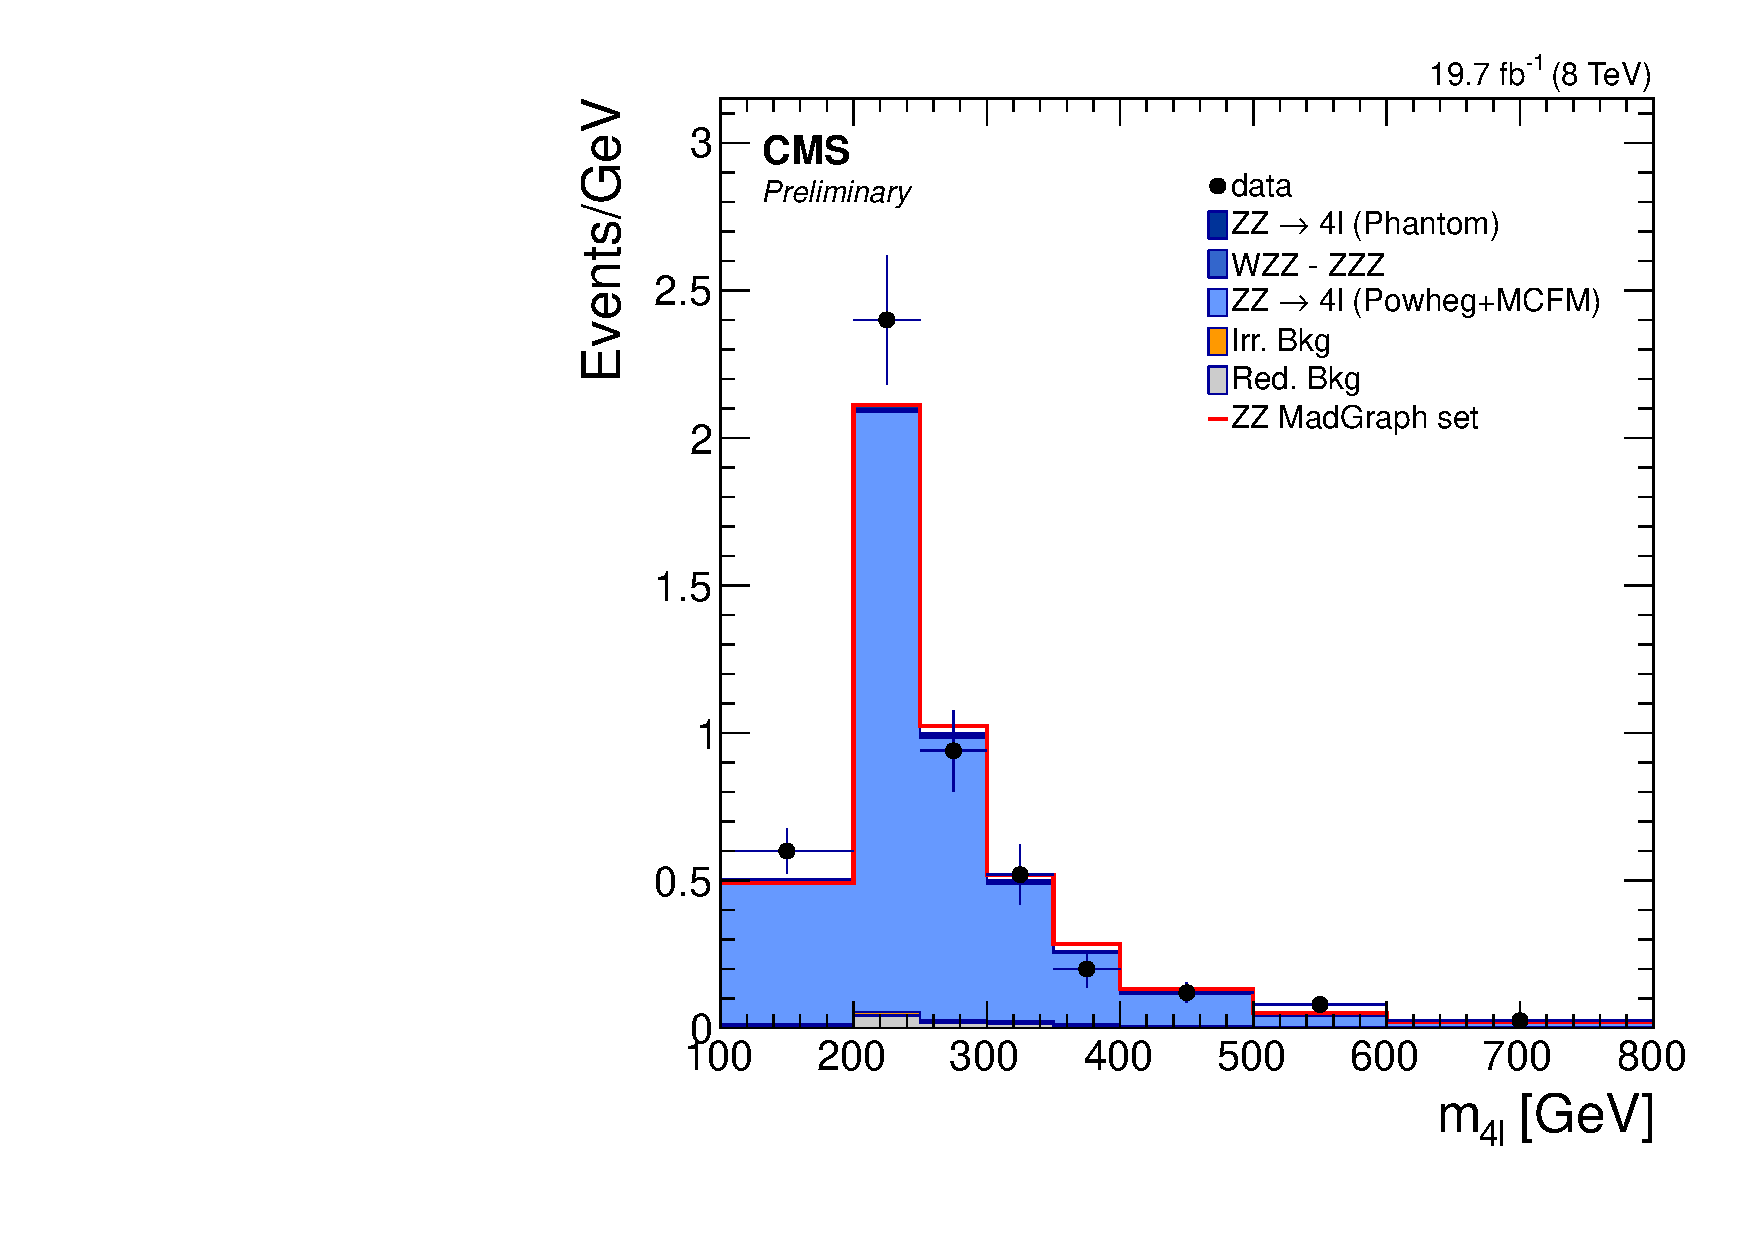
\includegraphics[width=\cmsFigWidth]{Figures/Mass_pow} 
    \caption{Different contributions to the distribution of the reconstructed four-lepton mass. Points represent the data, the stacked filled histogram represents the predictions for $ZZ$ signal and background contributions using \texttt{Powheg} samples to describe $q\bar{q}(qg)\to ZZ\to 4\ell$ processes (while for the stacked histogram outlined in red the \texttt{MadGraph} simulation is used).}
    \label{fig:sig_recoMass}
  \end{center}
\end{figure}
 
\begin{figure}[hbtp]
  \begin{center}
    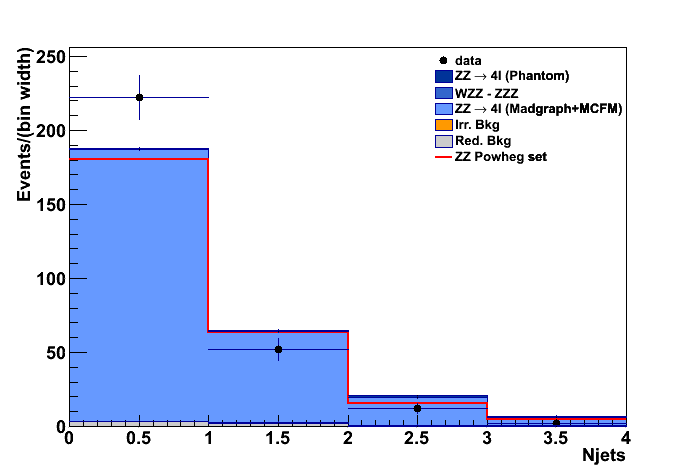
\includegraphics[width=\cmsFigWidth]{Figures/Jets_mad}
    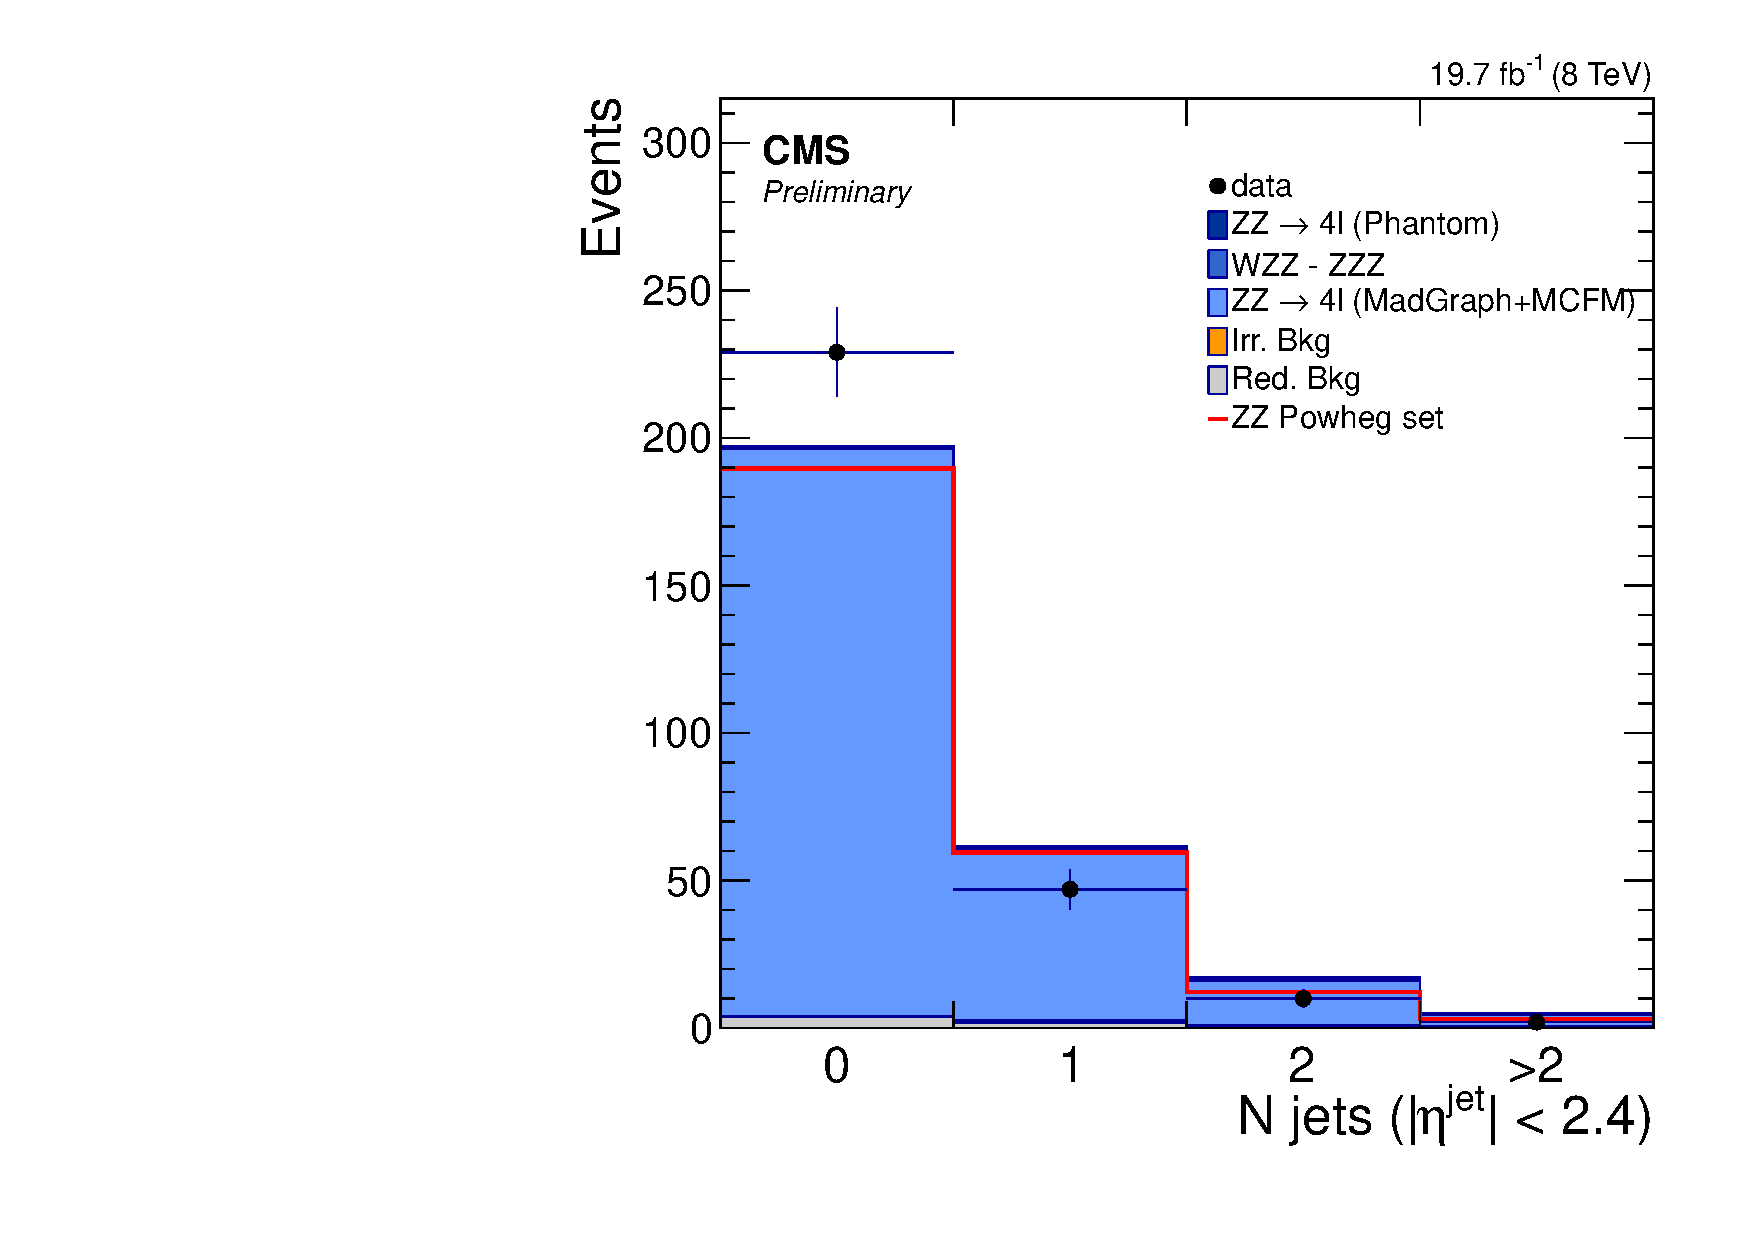
\includegraphics[width=\cmsFigWidth]{Figures/CentralJets_mad}
    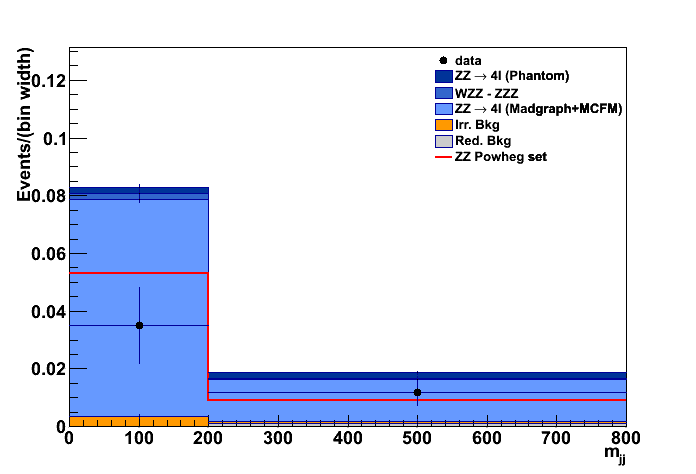
\includegraphics[width=\cmsFigWidth]{Figures/Mjj_mad}
    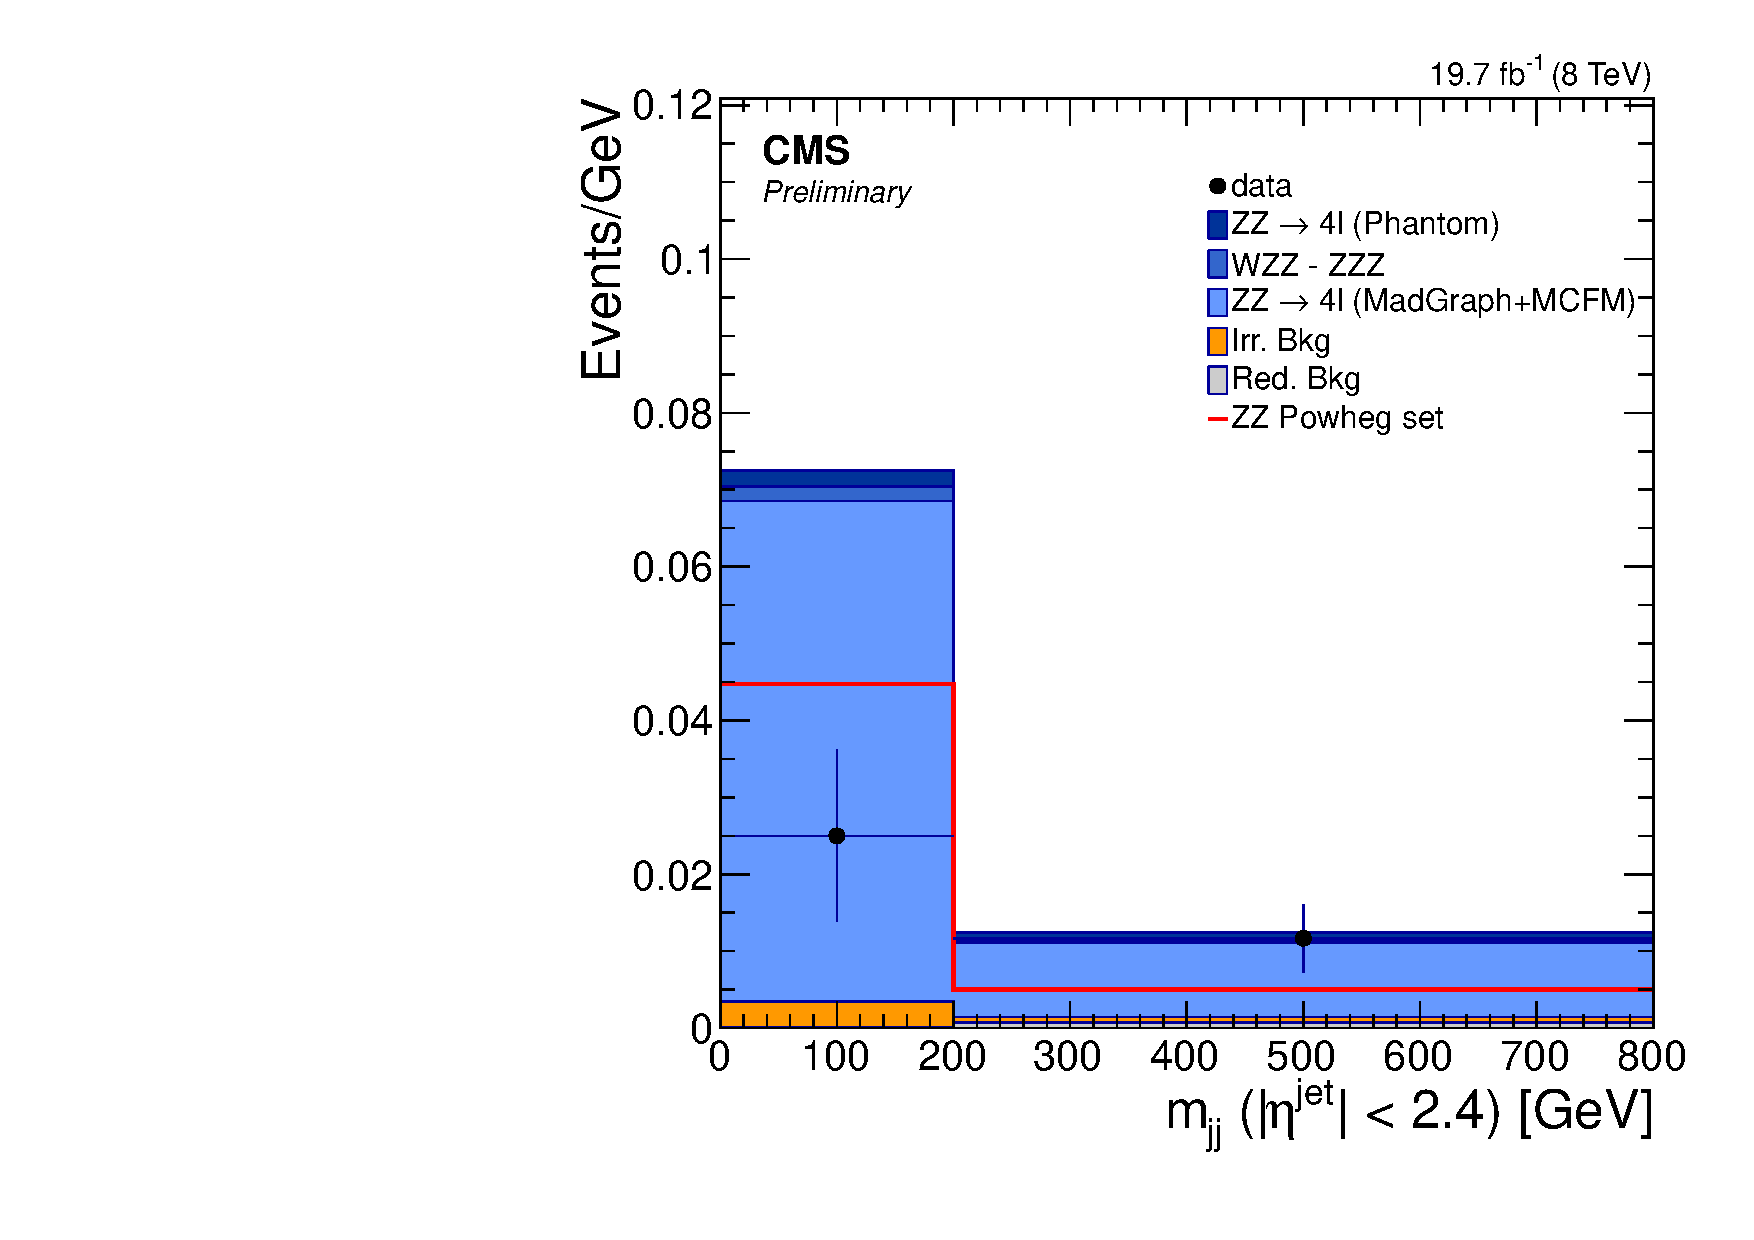
\includegraphics[width=\cmsFigWidth]{Figures/CentralMjj_mad} 
    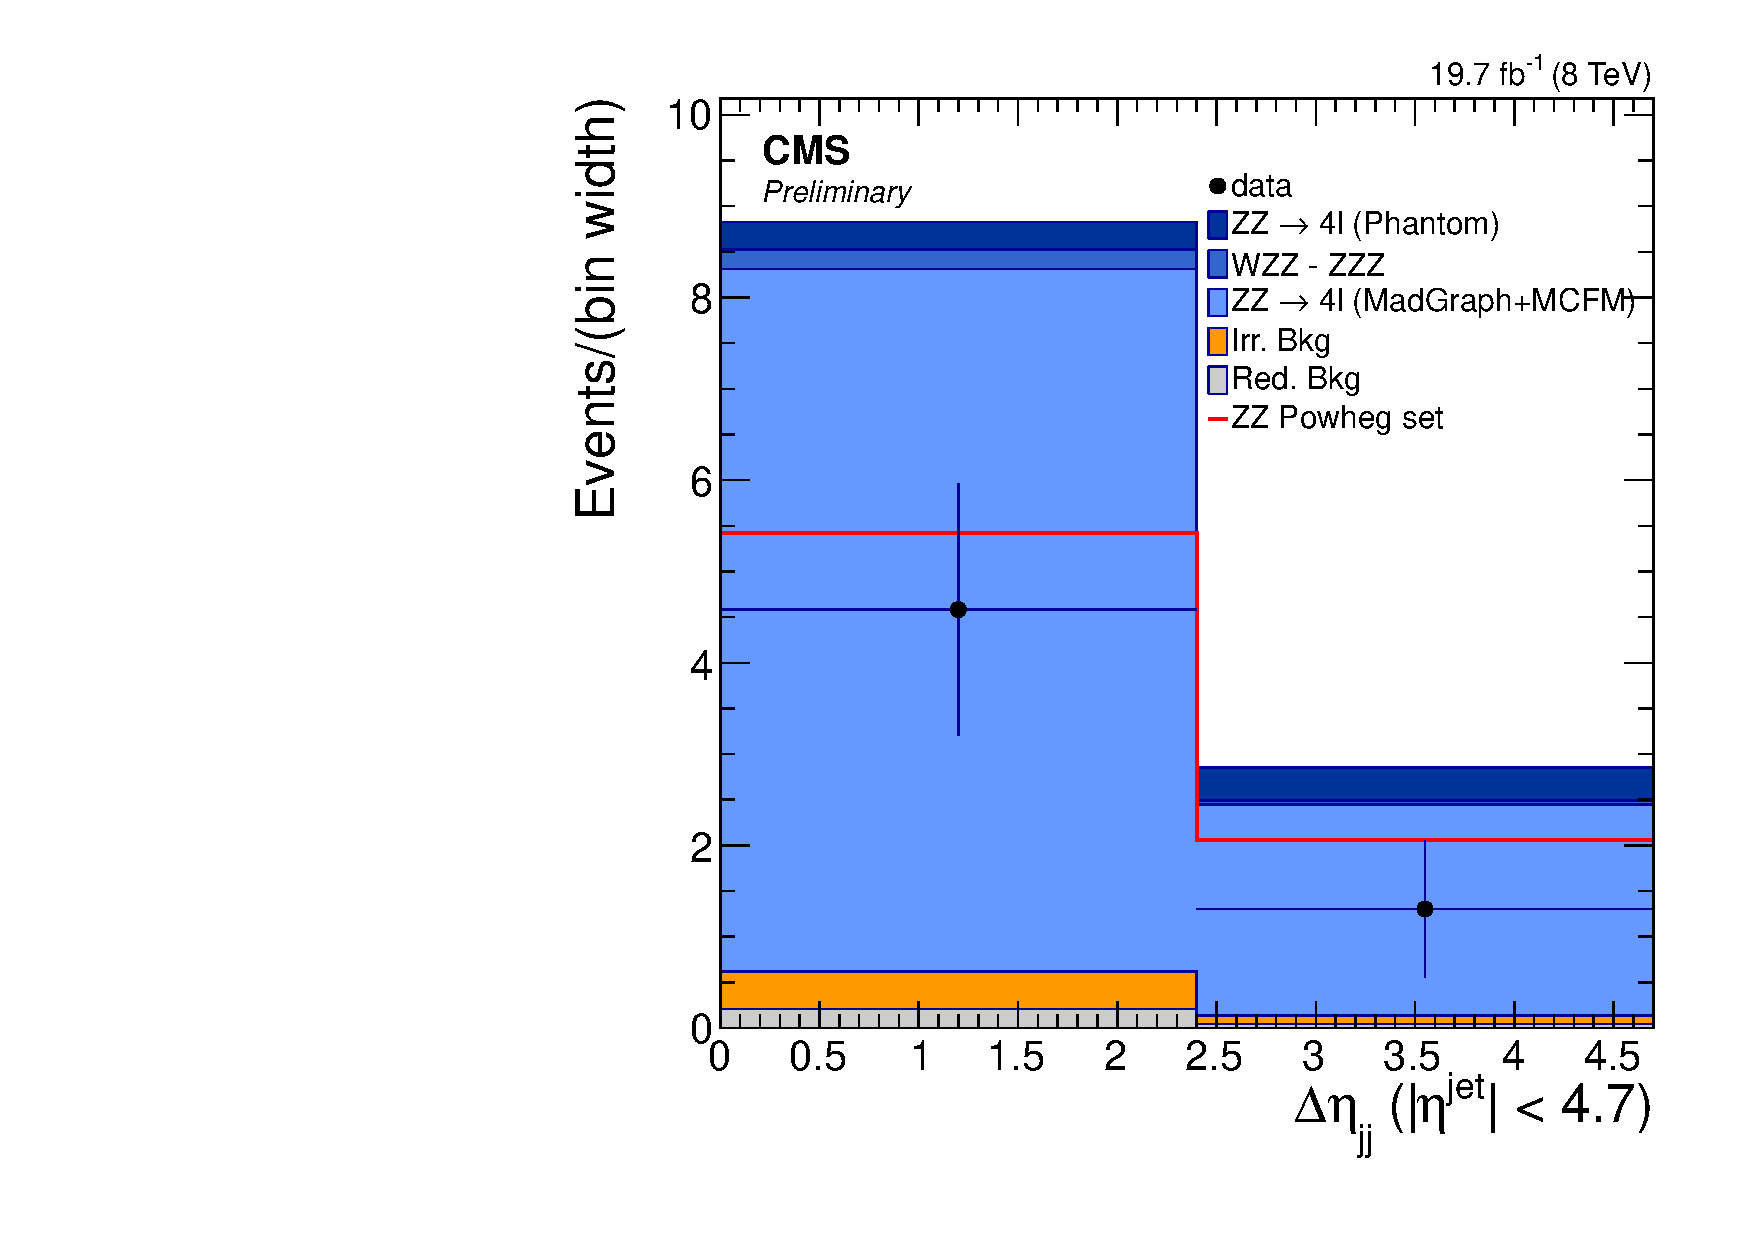
\includegraphics[width=\cmsFigWidth]{Figures/Deta_mad}  
    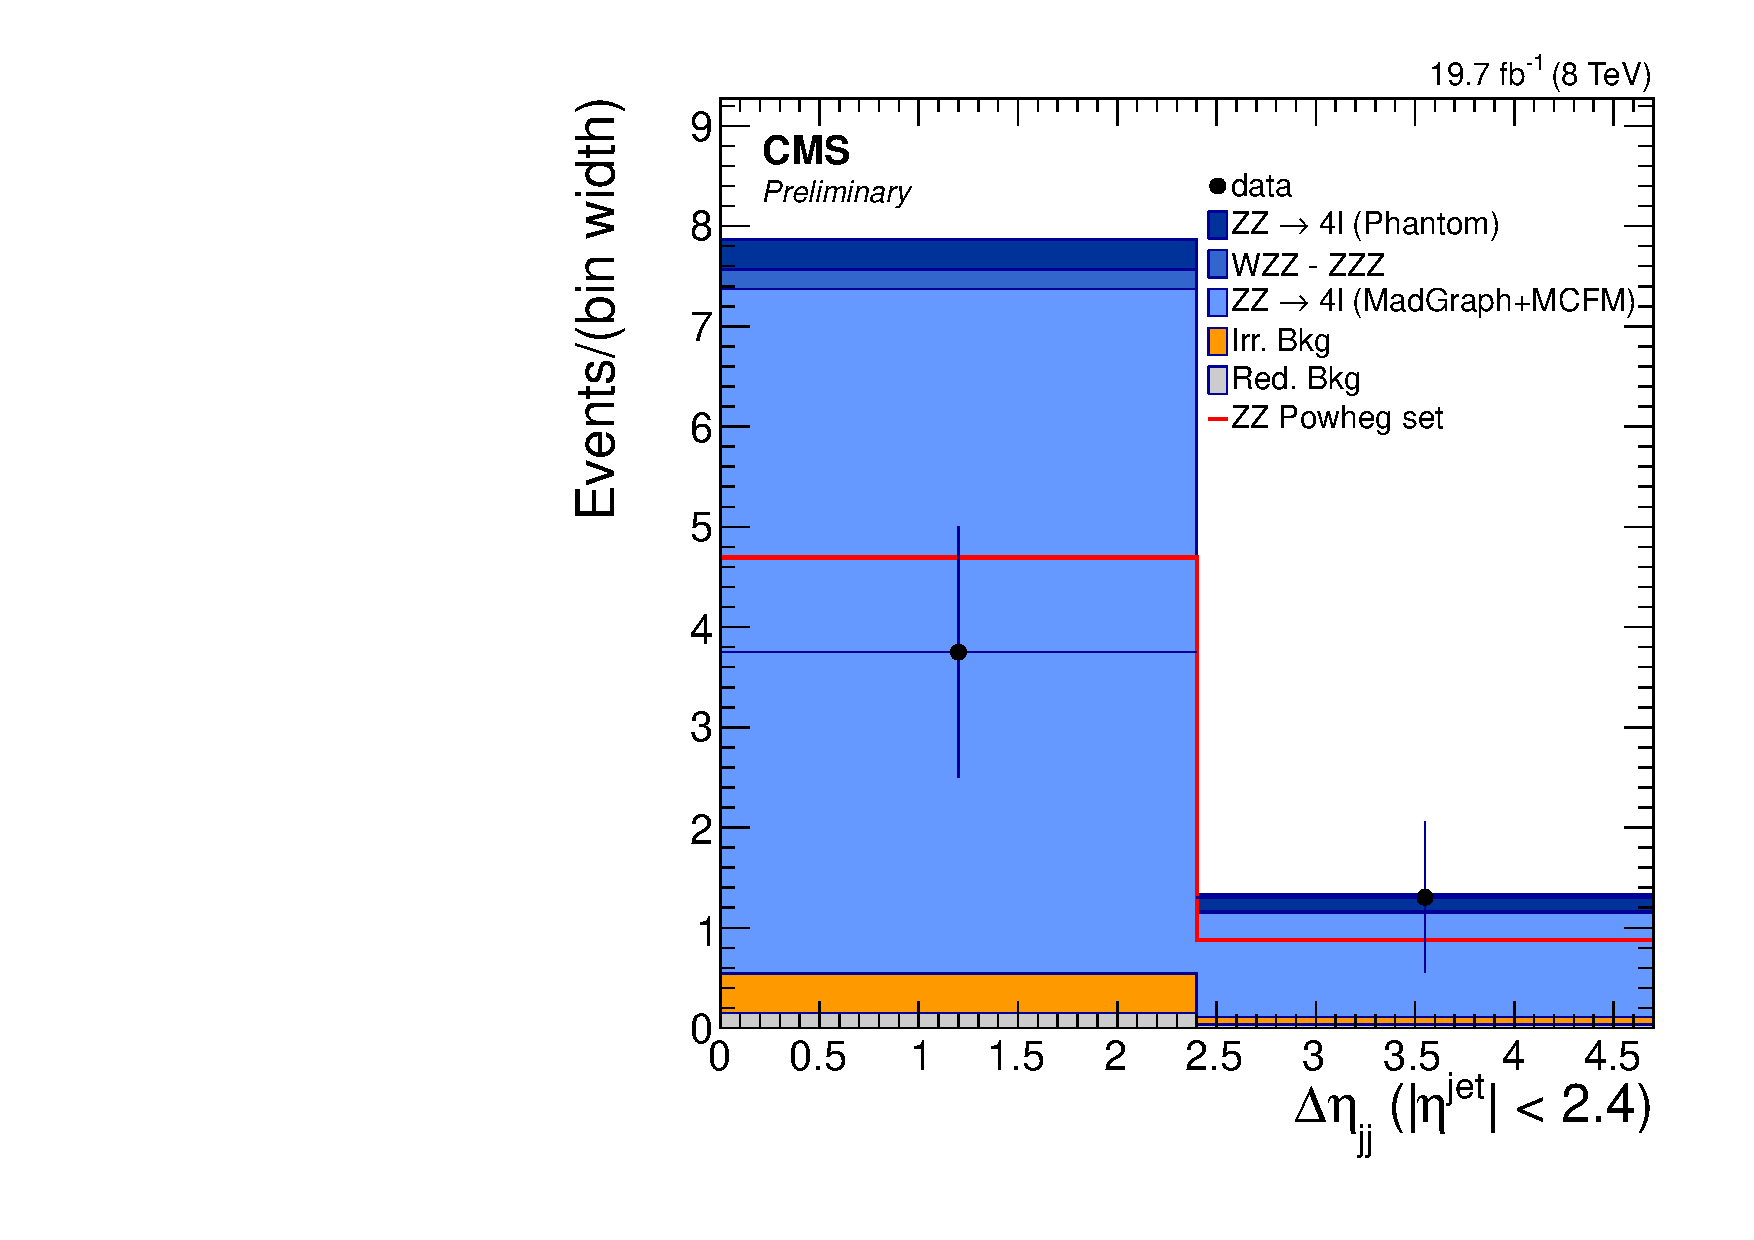
\includegraphics[width=\cmsFigWidth]{Figures/CentralDeta_mad}  
    \caption{Different contributions to the distribution of the reconstructed number of jets produced in the event (top), the invariant mass of the two most energetic jets (center) and the pseudorapidity interval between them (bottom), with $\eta^{jet} < 4.7$ on the left and $\eta^{jet} < 2.4$ on the right. Points represent the data, the stacked filled histogram represents the predictions for $ZZ$ signal and background contributions using \texttt{MadGraph} samples to describe $q\bar{q}(qg)\to ZZ\to 4\ell$ processes (while for the stacked histogram outlined in red the \texttt{Powheg} simulation is used).}
    \label{fig:sig_recoJJ}
  \end{center}
\end{figure}

\begin{figure}[hbtp]
  \begin{center} 
    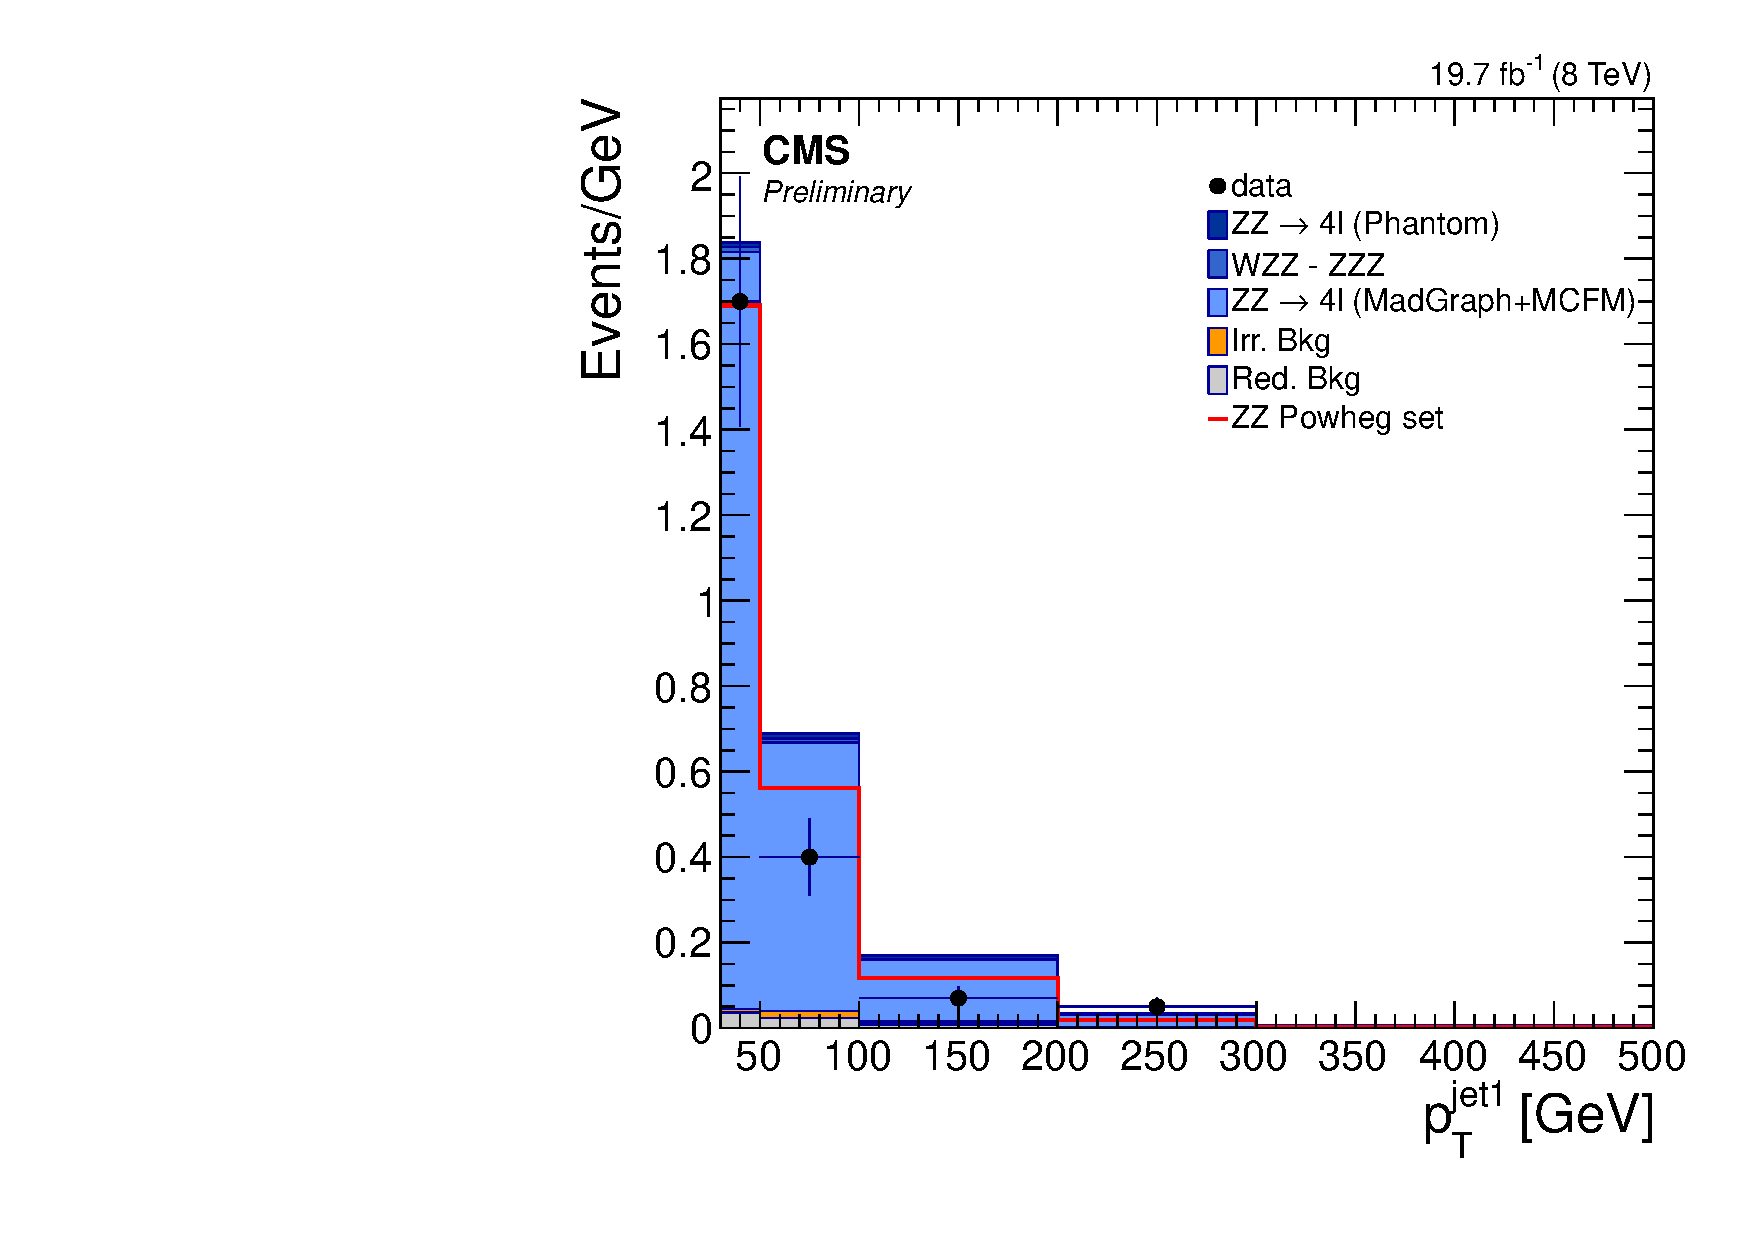
\includegraphics[width=\cmsFigWidth]{Figures/PtJet1_mad}
    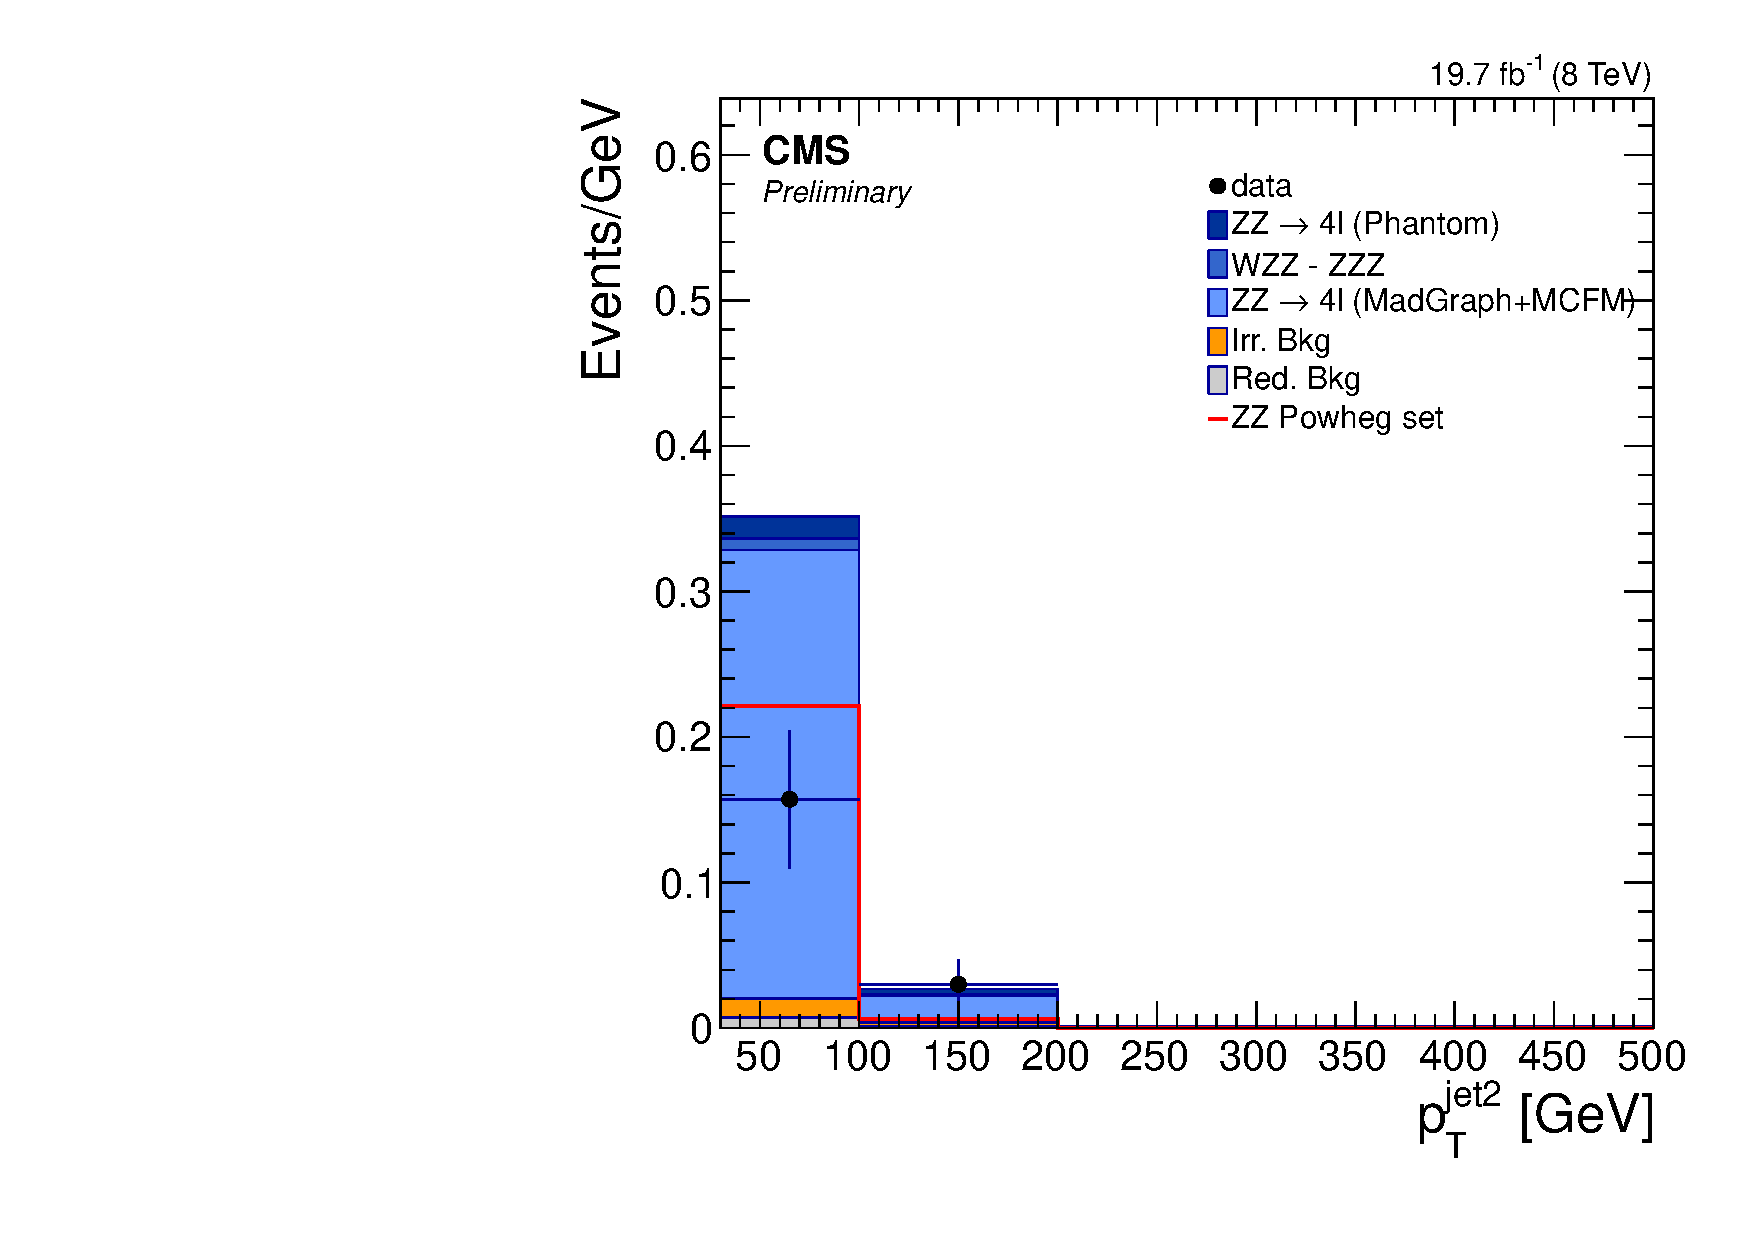
\includegraphics[width=\cmsFigWidth]{Figures/PtJet2_mad} 
    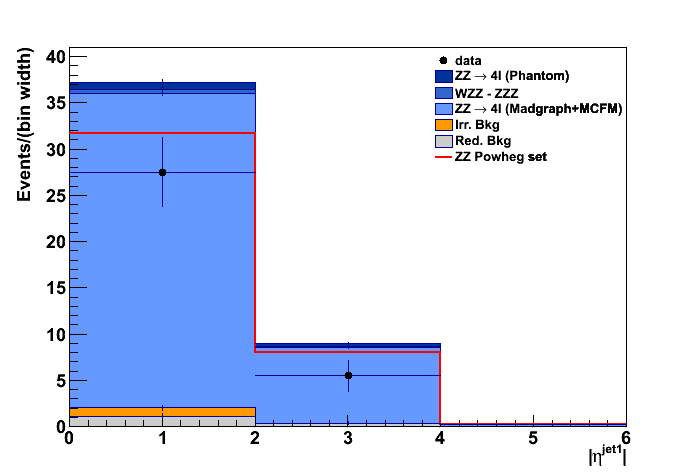
\includegraphics[width=\cmsFigWidth]{Figures/EtaJet1_mad}
    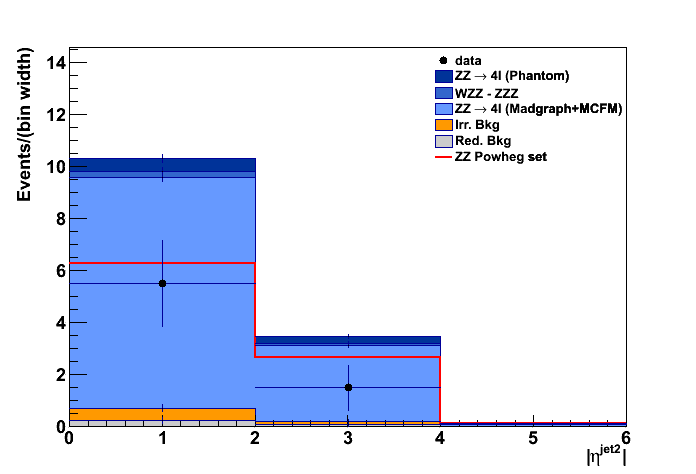
\includegraphics[width=\cmsFigWidth]{Figures/EtaJet2_mad}
    \caption{Different contributions to the distribution of the reconstructed transverse momentum (top) and pseudorapidity (bottom) of the leading (left) and  sub-leading jet (right). Points represent the data, the stacked filled histogram represents the predictions for $ZZ$ signal and background contributions using \texttt{MadGraph} samples to describe $q\bar{q}(qg)\to ZZ\to 4\ell$ processes (while for the stacked histogram outlined in red the \texttt{Powheg} simulation is used).}
    \label{fig:sig_recoPt}
  \end{center}
\end{figure}


\begin{figure}[hbtp]
  \begin{center}
   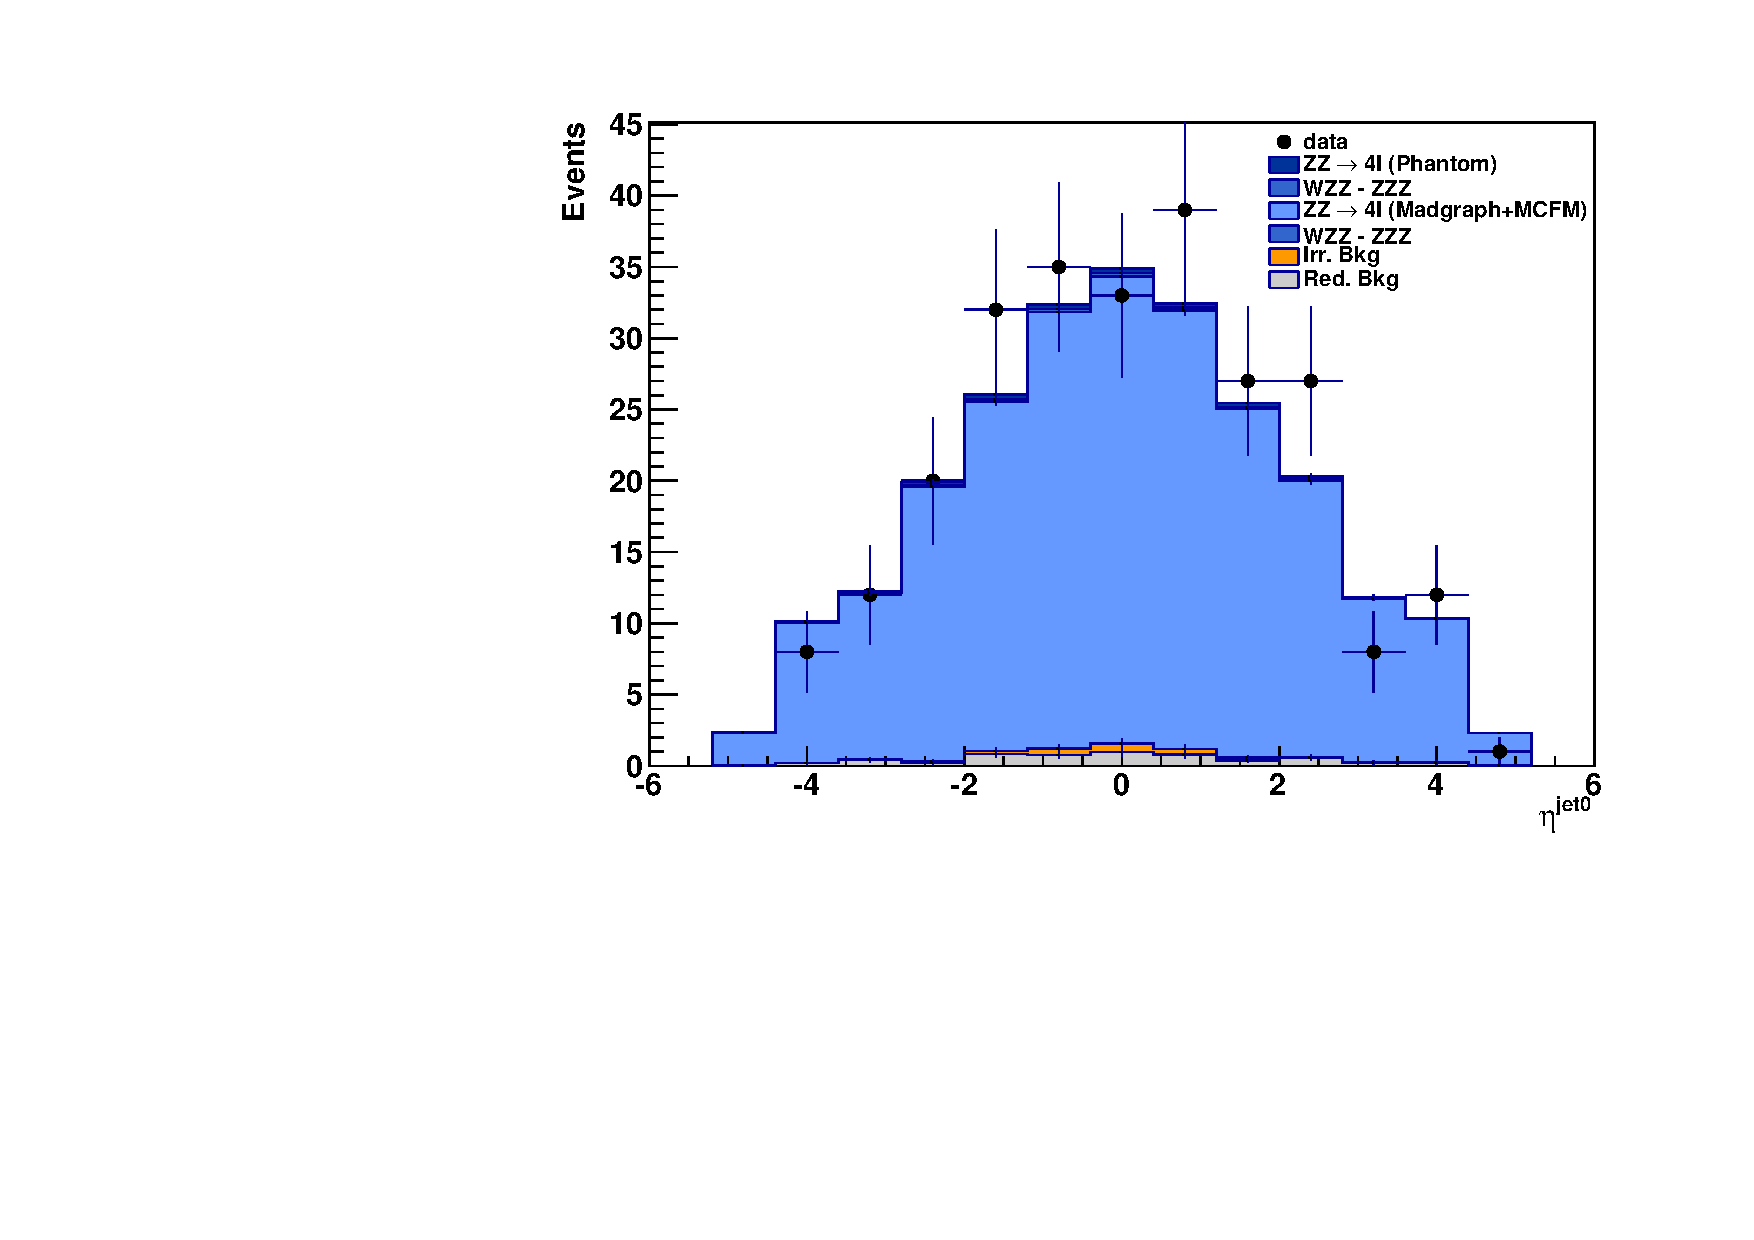
\includegraphics[width=0.8\cmsFigWidth]{Figures/Eta0_mad}    
   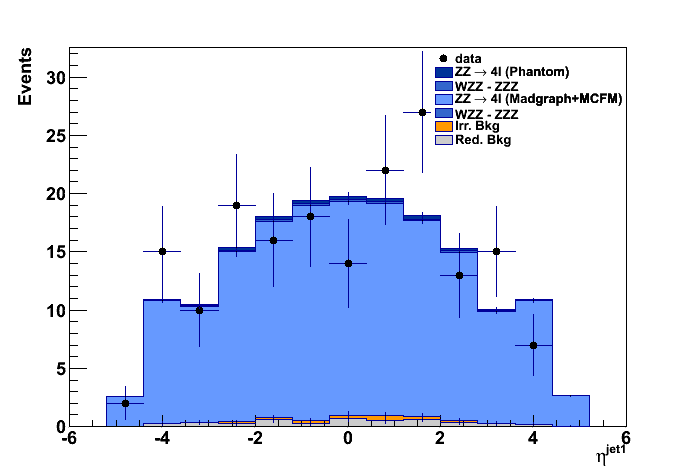
\includegraphics[width=0.8\cmsFigWidth]{Figures/Eta1_mad}
   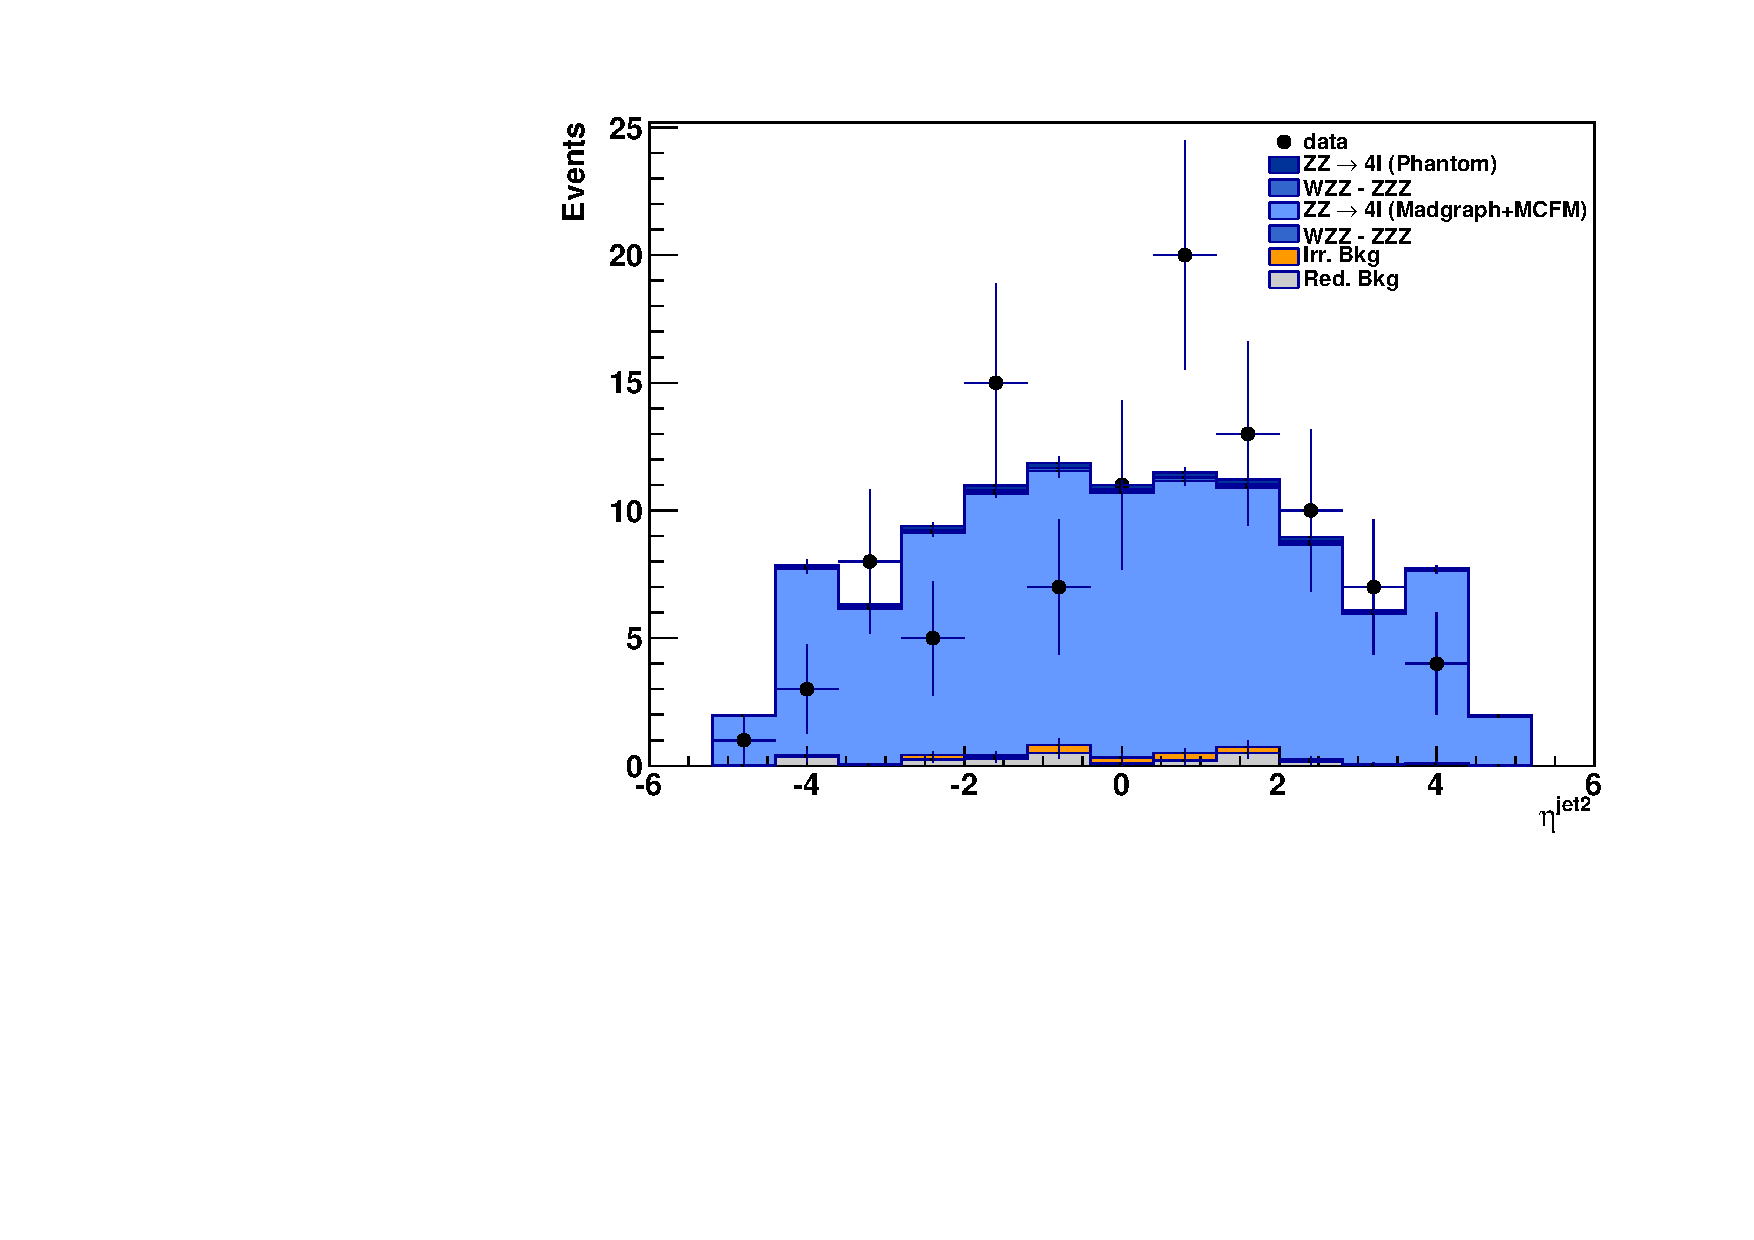
\includegraphics[width=0.8\cmsFigWidth]{Figures/Eta2_mad}
   \caption{Different contributions to the $\eta$-distribution of the most energetic (\cmsLeft), second most energetic (center) and third most energetic (\cmsRight) jet in the event, considering $p_T^{jet}> 10~\mathrm{GeV}$}
   \label{fig:eta_jets}
  \end{center}
\end{figure}
\begin{figure}[hbtp]
  \begin{center}
   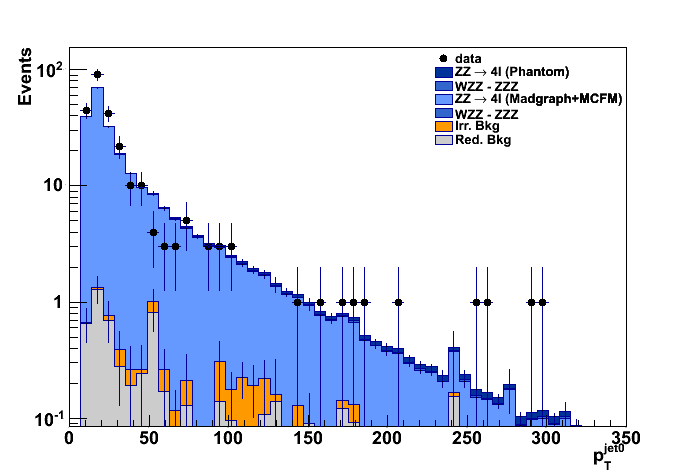
\includegraphics[width=0.8\cmsFigWidth]{Figures/Pt0_mad_log}    
   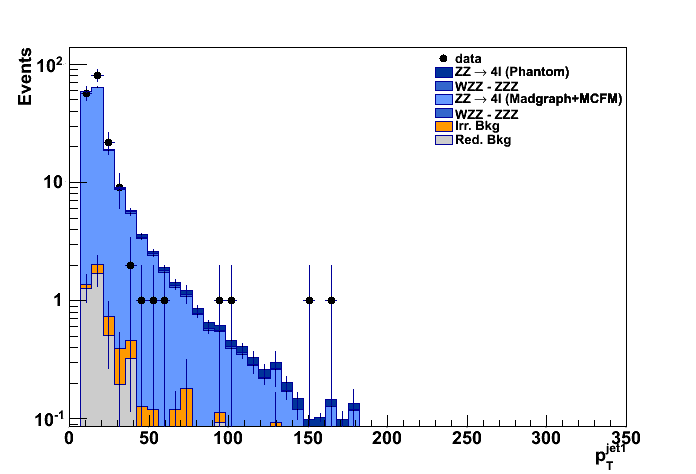
\includegraphics[width=0.8\cmsFigWidth]{Figures/Pt1_mad_log}
   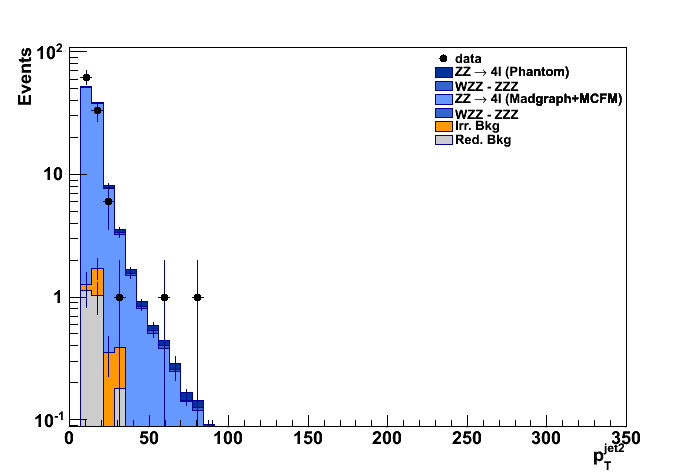
\includegraphics[width=0.8\cmsFigWidth]{Figures/Pt2_mad_log}
   \caption{Different contributions to the $p_{T}$-distribution of the most energetic (\cmsLeft), second most energetic (center) and third most energetic (\cmsRight) jet in the event, considering  $p_T^{jet}> 10~\mathrm{GeV}$.}
   \label{fig:pt_jets}
  \end{center}
\end{figure}
Table~\ref{tab:xs} lists the total cross-section obtained from each individual decay channel as well as the
total cross-section based on the combination of all channels. The measured cross-section agrees
with the theoretical value of $7.5\pm 0.5$ pb calculated with \texttt{MCFM 6.6}. In this calculation, the
contribution from $q\bar{q} \to ZZ$ is obtained at NLO, while the smaller contribution (approximately
6\%) from $ gg \to ZZ$ is obtained at LO.

\begin{table*}[htbH]
\begin{center}
\topcaption{The signal yield is obtained by subtracting from the observed yield the expected background events. Statistical uncertainties are reported.
\label{tab:sig_yields}}
\begin{tabular}{lcccc}
\hline Final state & Observed data& Irreducible background & Reducible background & Final yield\\
\hline $ZZ\to 4\mu $ & $ 80 \pm 8.9 $ & $ 0.52 \pm 0.10 $ & $ 0.92 \pm 0.61 $ & $ 78.6 \pm 8.9$ \\ 
$ZZ\to 4e $ & $56 \pm 7.5 $ & $ 0.21 \pm 0.06 $ & $ 1.93 \pm 0.72 $ & $ 54.0 \pm 7.5 $\\
$ZZ\to 2e2\mu$ & $ 152 \pm 12 $ & $ 1.16 \pm 0.15 $ & $ 3.3 \pm 1.1 $ & $ 148 \pm 12 $\\
\hline
\textbf{$ZZ\to 4\ell$} & $ 288 \pm 17 $ & $1.89 \pm 0.19 $ & $ 6.2 \pm 1.4 $ & $ 281 \pm17 $ \\ 
\hline 
\end{tabular}
\end{center}
\end{table*}

%\begin{table*}[htbH]
%\begin{center}
%\topcaption{The total $ZZ$ production cross-section as measured in each decay channel and for the
%combination of all channels.
%\label{tab:xs}}
%\begin{tabular}{lc}
%\hline Final state & Total cross-section [pb]\\
%\hline $ZZ\to 4\mu $ & $7.5\pm 0.9$ (stat.) $\pm 0.3$ (syst.)\\
%$ZZ\to 4e $ &  $7.4\pm 1.0$ (stat.) $\pm 0.3$ (syst.)\\
%$ZZ\to 2e2\mu$ & $8.3\pm 0.7$ (stat.) $\pm 0.4$ (syst.)\\
%\hline
%\textbf{$ZZ\to 4\ell$} &  $7.6\pm 0.5$ (stat.) $\pm 0.3$ (syst.)\\
%\hline \\
%\end{tabular}
%\end{center}
%\end{table*}
\begin{table*}[htbH]
\begin{center}
\caption{The total $ZZ$ production cross-section as measured in each decay channel and for the
combination of all channels in the fiducial region $60< m_{Z_{1}}, m_{Z_{}} < 120~\mathrm{GeV}$.}
\label{tab:xs}
%\scalebox{1.5\columnwidth}{!}{
%\doublespacing{
\begin{tabular}{lc}
\hline Process & Total cross-section [pb]\\
\hline $pp\to ZZ(4\mu) $ & $7.46\pm 0.86~\mathrm{(stat.)}^{+0.45}_{- 0.47}~\mathrm{(syst.)}$\\
$pp\to ZZ(4e) $ &  $7.32\pm 1.02~\mathrm{(stat.)}^{+0.59}_{- 0.62}~\mathrm{(syst.)}$\\
$pp\to ZZ(2e2\mu)$ & $8.22\pm 0.70~\mathrm{(stat.)}^{+0.59}_{- 0.61}~\mathrm{(syst.)}$\\
\hline
\textbf{$pp\to ZZ(4\ell)$} & $7.76 \pm 0.48~\mathrm{(stat.)}^{+0.47}_{- 0.47}~\mathrm{(syst.)}$ \\
\hline \\
\end{tabular}%}
\end{center}
\end{table*}
The fiducial region in which the cross-section is extracted, defined requiring two $Z$ bosons with mass between 60 and 120 GeV, is much wider with respect to the region in which events are really measured, limited by the active volume of the detector, as shown by the low values of $A\cdot \epsilon$. In order to obtain a measurement closer to what is effectively reconstructed by the detector, a \emph{tight fiducial region} is defined as follows:
\begin{itemize}
\item $60 < m_{Z_1},m_{Z_2} < 120~\mathrm{GeV}$;
%\item $m_{4\ell} > 100~\mathrm{GeV}$;
\item at least one lepton with $p_T > 20~\mathrm{GeV}$ and another one with $p_T > 10~\mathrm{GeV}$;
\item electrons must have $p_T^e > 7~\mathrm{GeV}$ and $|\eta^e|<2.5$;
\item muons must have $p_T^{\mu} > 5~\mathrm{GeV}$ and $|\eta^{\mu}|<2.4.$
\end{itemize}
The last three requirements correspond to the $\eta$ and $p_T$-acceptance of the detector and are the same selection criteria demanded when leptons are built, while the first requirement corresponds to the definition of the wider region applied for the previous inclusive measurement. The formula used in this case is
$$\sigma_{ZZ} = \frac{N_{data}-N_{bkg}}{\mathcal{L}\cdot A \cdot \epsilon},$$
where the branching-ratio factor is removed in order to obtain the cross-section of the $pp\to ZZ\to 4\ell$ process, and the new values of $ A \cdot \epsilon$ are reported in Table~\ref{tab:Aeps_tight}. The cross-section measurements obtained in this tight region are listed in Table~\ref{tab:tightxs}.
\begin{table*}[htbH]
\begin{center}
\topcaption{$A\cdot \epsilon$ for the three final states used in the $pp\to ZZ \to 4\ell$ cross-section measurement in the tight fiducial region.
The values reported are a product of the detector geometrical acceptance and
the object reconstruction and event identification efficiency. \label{tab:Aeps_tight}}
\begin{tabular}{cc}
\hline Final State & $A\cdot\epsilon$\\
\hline $4\mu$ & 84 \%  \\
$4e$ & 55\%\\
$2e2\mu$ & 69\%\\
\hline
\end{tabular}
\end{center}
\end{table*}
\begin{table*}[htbH]
\begin{center}
\topcaption{The total $ZZ$ production cross-section as measured in each decay channel and for the
combination of all channels in the tight fiducial region.
\label{tab:tightxs}}
\begin{tabular}{lc}
\hline Final state & Total cross-section [fb]\\
\hline $ZZ\to 4\mu $ & $4.74\pm 0.54$ (stat.) $^{+0.17}_{-0.18}$ (syst.)\\
$ZZ\to 4e $ &  $4.99\pm 0.69$ (stat.) $^{+0.32}_{-0.35}$ (syst.)\\
$ZZ\to 2e2\mu$ & $10.77\pm 0.90$ (stat.) $^{+0.55}_{-0.59}$ (syst.)\\
\hline
\textbf{$ZZ\to 4\ell$} &  $20.50\pm 1.26$ (stat.) $^{+0.82}_{-0.85}$ (syst.)\\
\hline \\
\end{tabular}
\end{center}
\end{table*}

\begin{figure}[hbtp]
  \begin{center}
    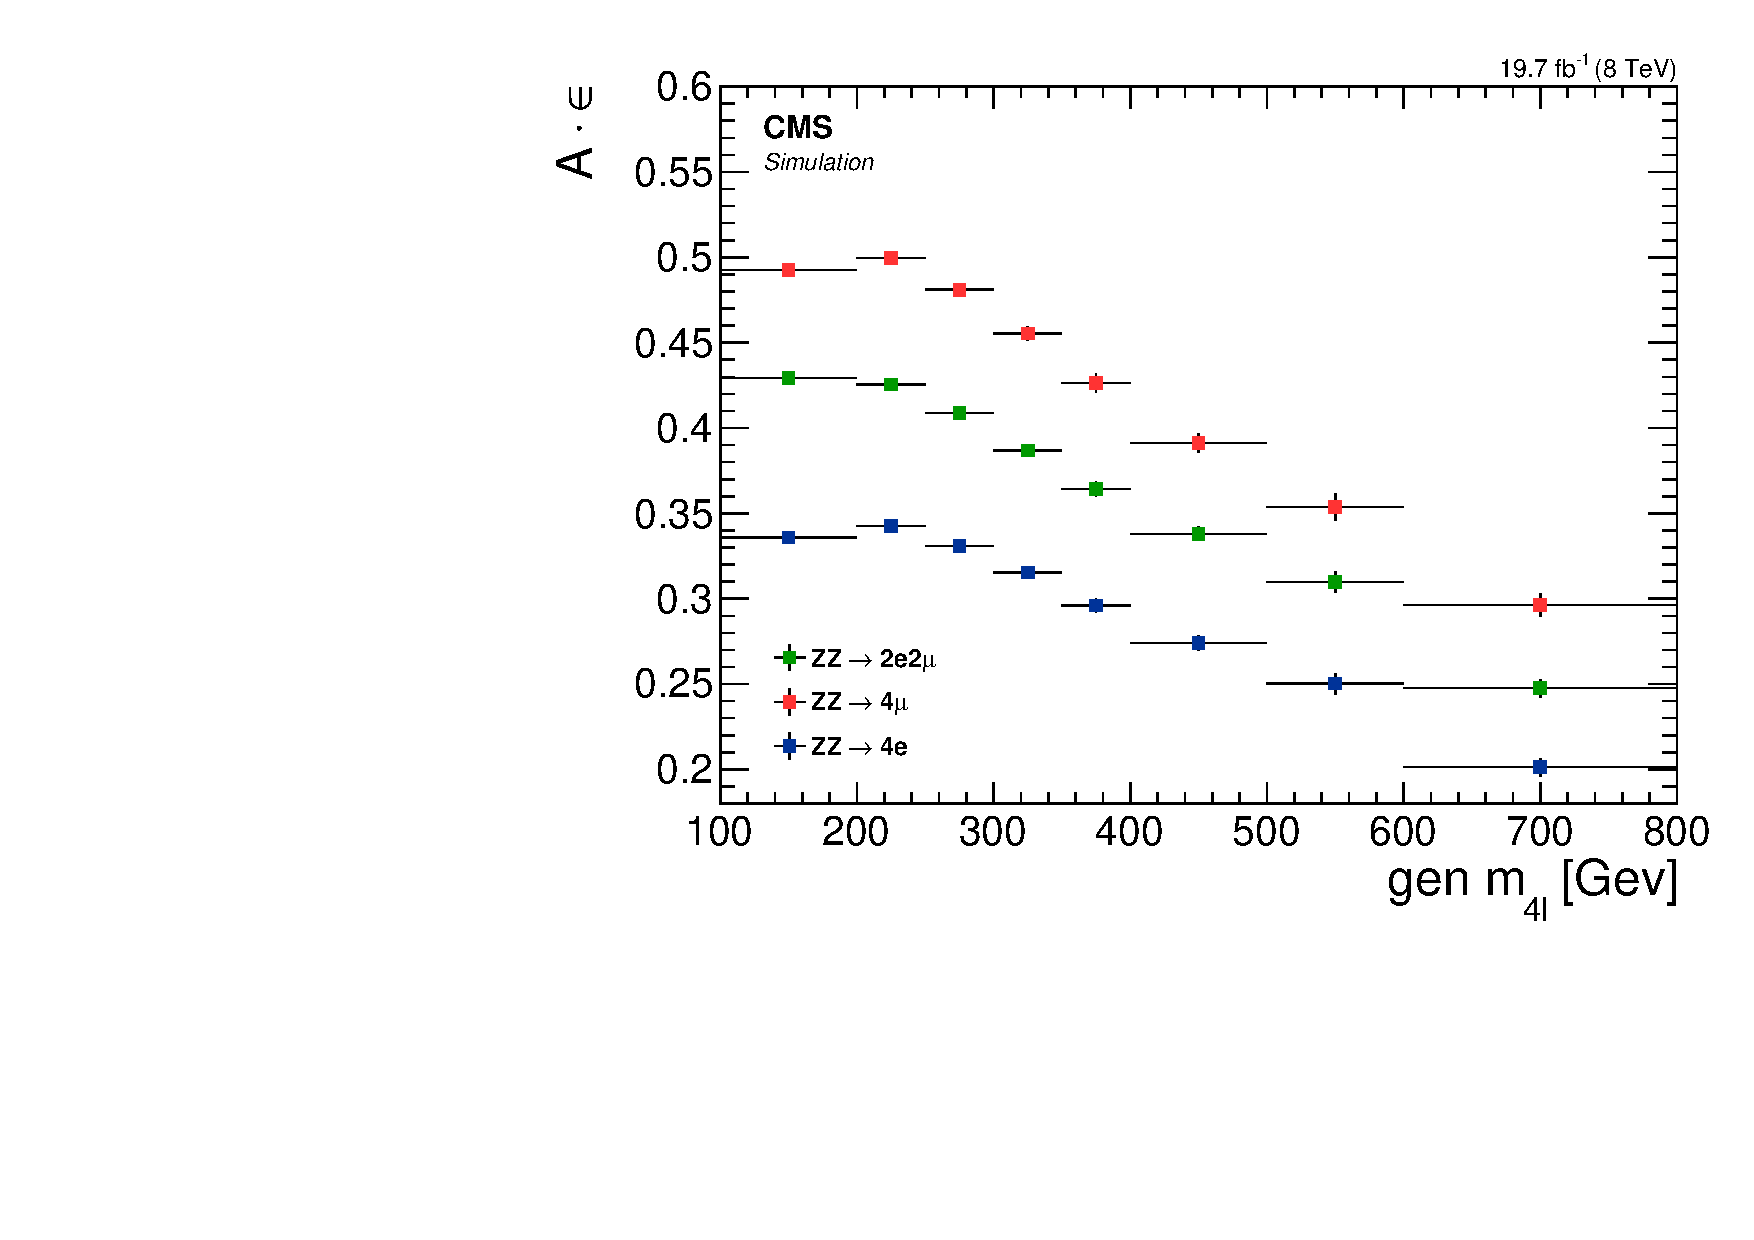
\includegraphics[width=\cmsFigWidth]{Figures/DiffAcceptance_Mass_Pow}
    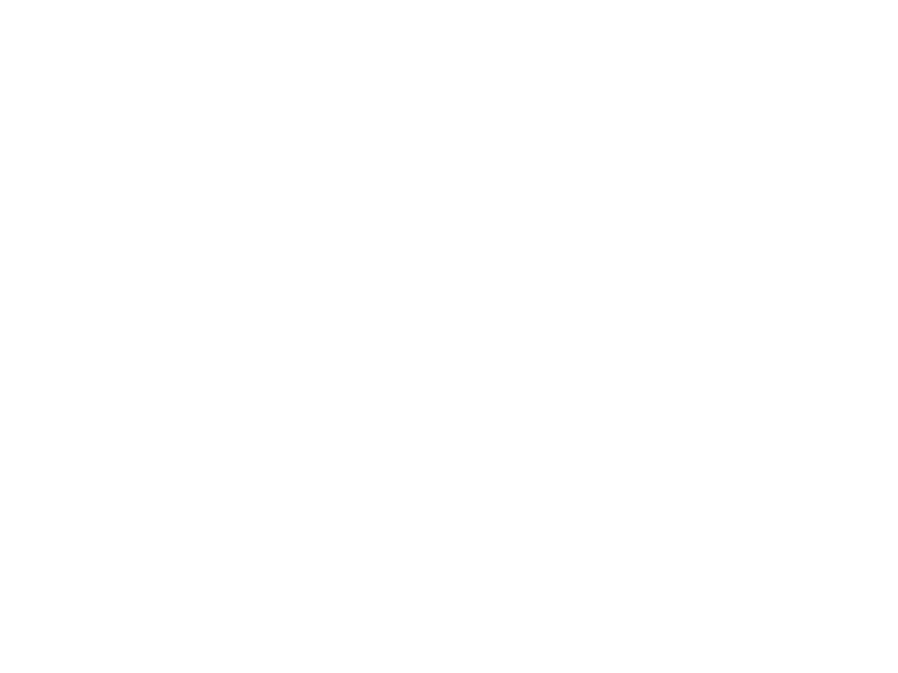
\includegraphics[width=\cmsFigWidth]{Figures/DiffAcceptance_Jets_Mad}
    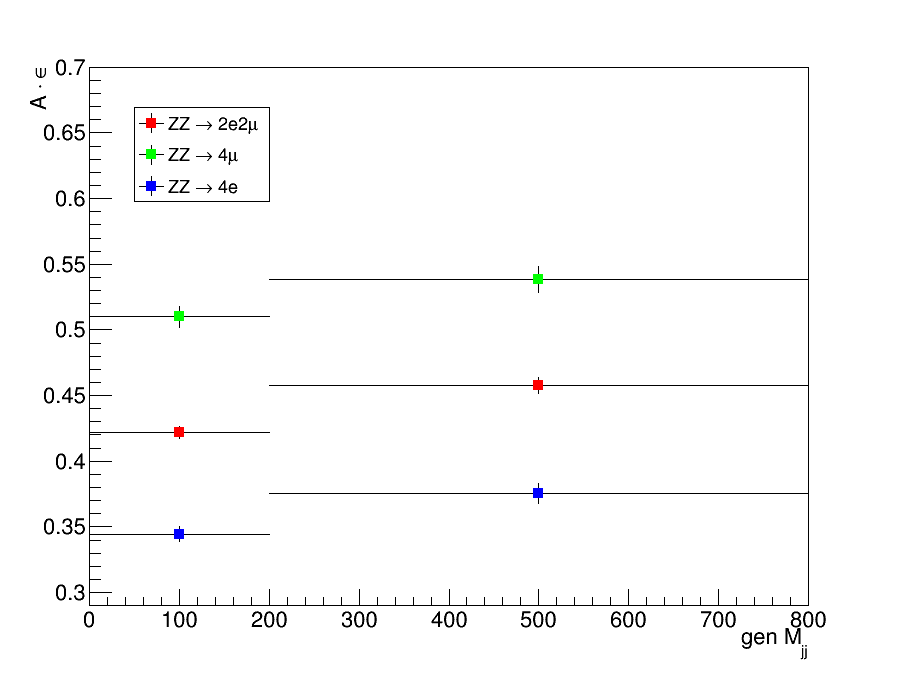
\includegraphics[width=\cmsFigWidth]{Figures/DiffAcceptance_Mjj_Mad}
    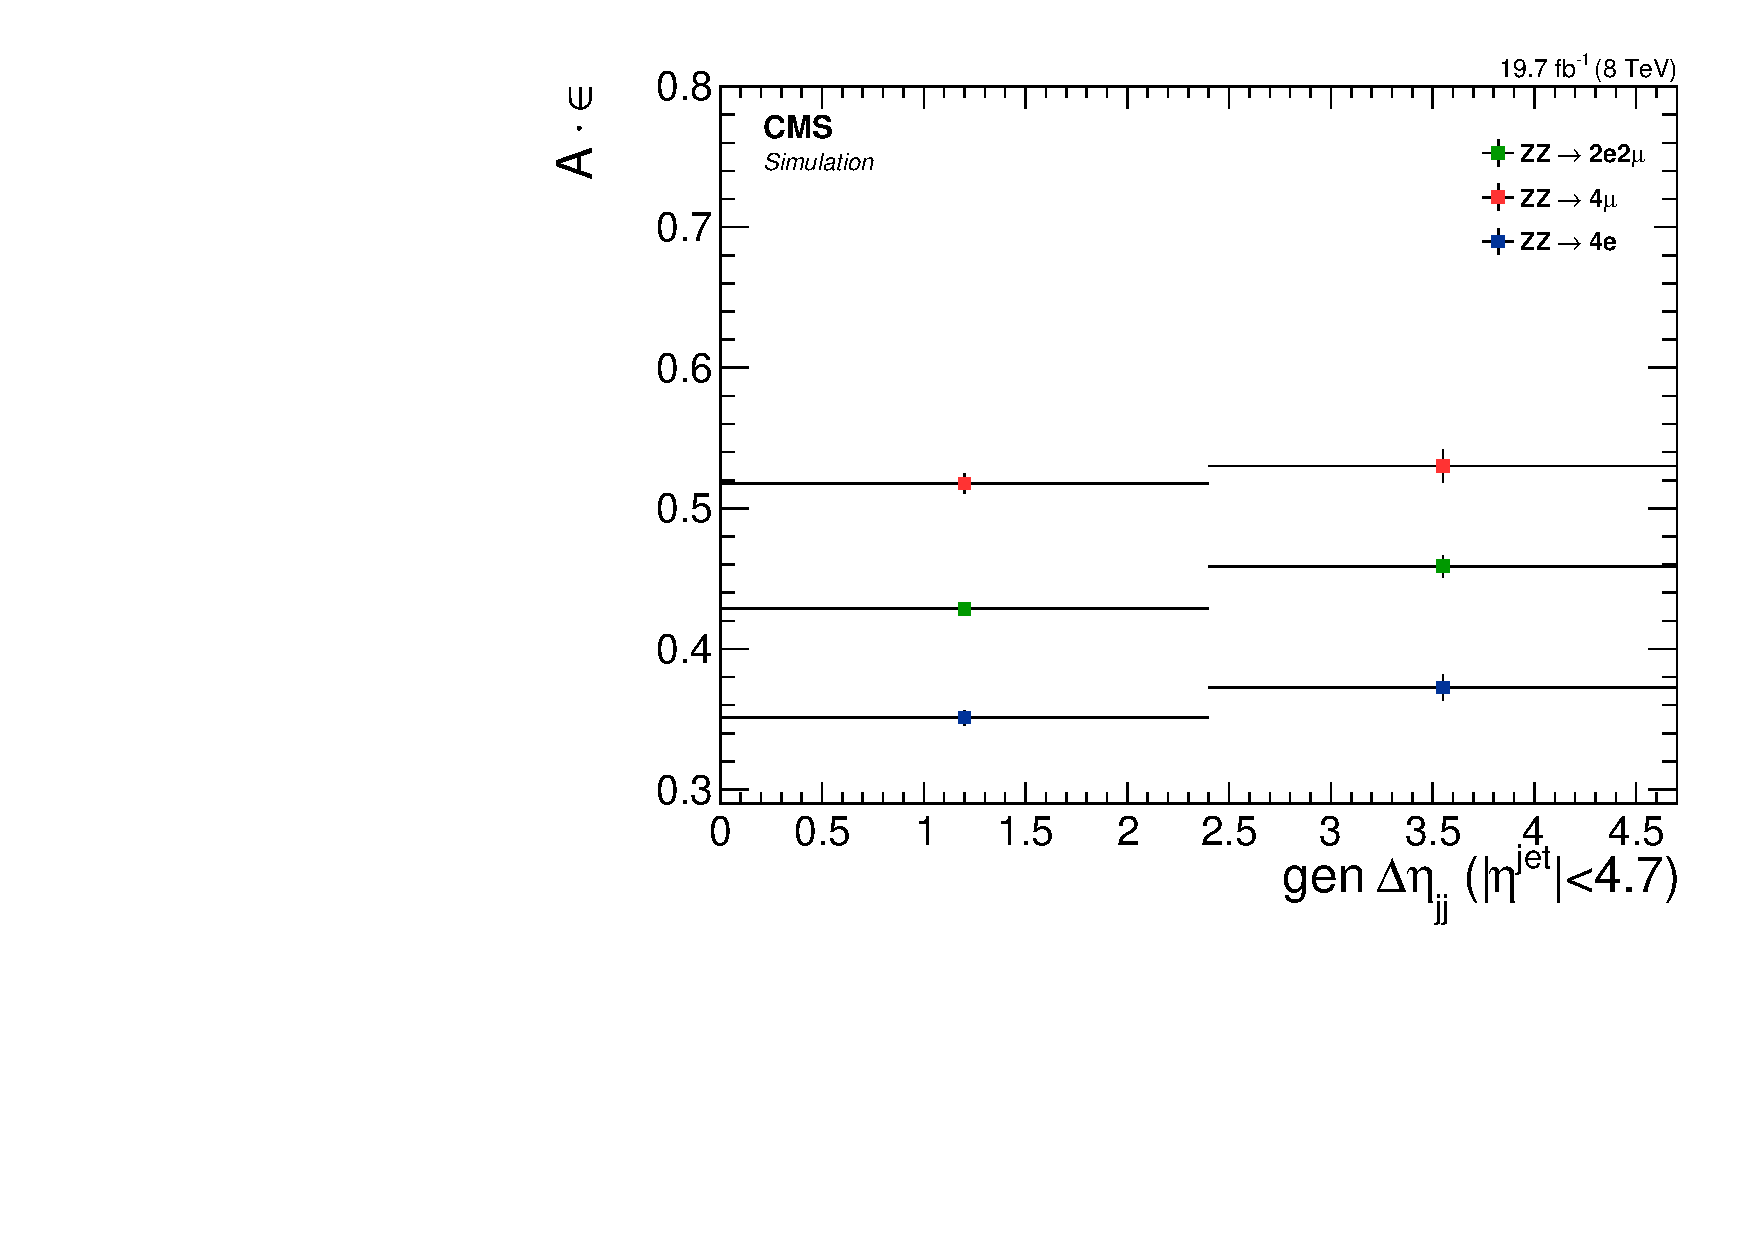
\includegraphics[width=\cmsFigWidth]{Figures/DiffAcceptance_Deta_Mad}
    %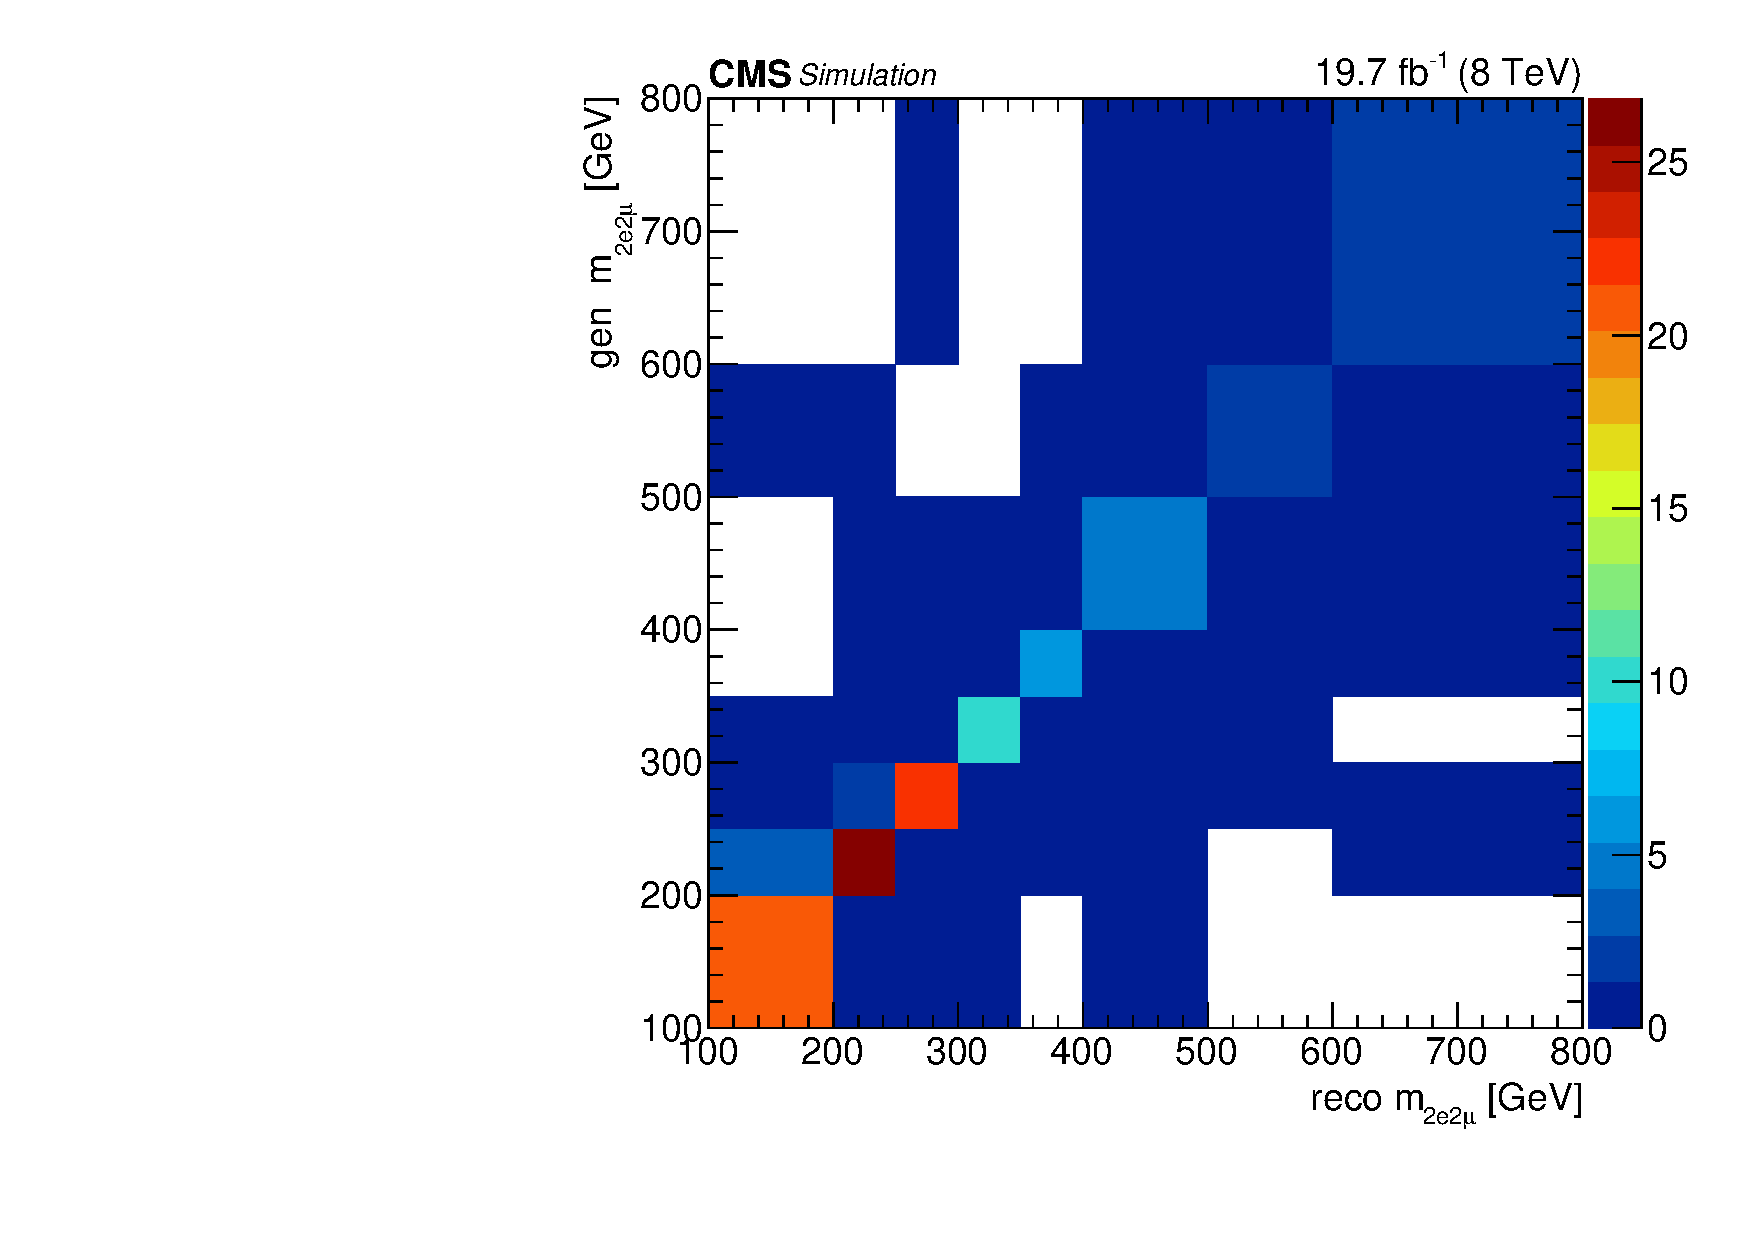
\includegraphics[width=\cmsFigWidth]{Figures/ResMat_qqggJJ_Mass_ZZTo2e2m_st_01_Pow}     
 %   to generate (a) and (b) labels under the figures, you can use subfloat, but this is not recommended: takes too much space
 %   \subfloat[]{
\includegraphics[width=0.2\textwidth]{CMS-bw-logo}}\subfloat[]{
\includegraphics[width=0.2\textwidth]{CMScol}}
    \caption{Acceptance ($A \cdot \epsilon$) computed in the wider fiducial region as a function of $m_{ZZ}$  (top left), $N\ jets$  (top right), $m_{jj}$ (bottom left) and $\Delta\eta_{jj}$
distributions, according to the final state: 
      $4\mu$ (green), $4e$ (blue), $2e2\mu$  (red). Distributions are obtained using the  \texttt{Powheg} set of samples for  $m_{ZZ}$ and 
     the  \texttt{MadGraph} set of samples for the other variables.} 
    \label{fig:A_diff}
  \end{center}
\end{figure}
\begin{figure}[hbtp]
  \begin{center}
    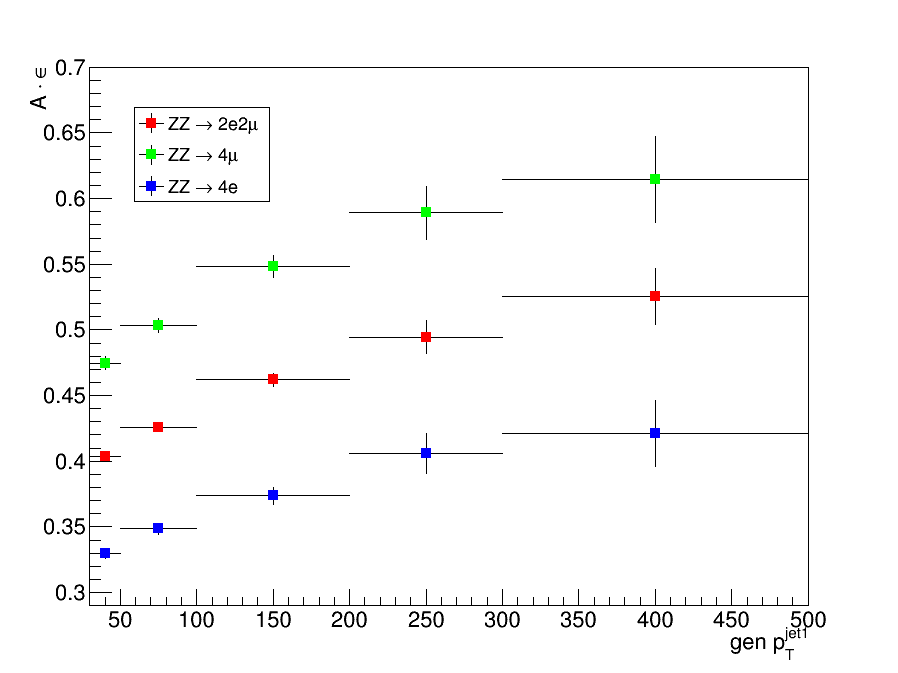
\includegraphics[width=\cmsFigWidth]{Figures/DiffAcceptance_PtJet1_Mad}
    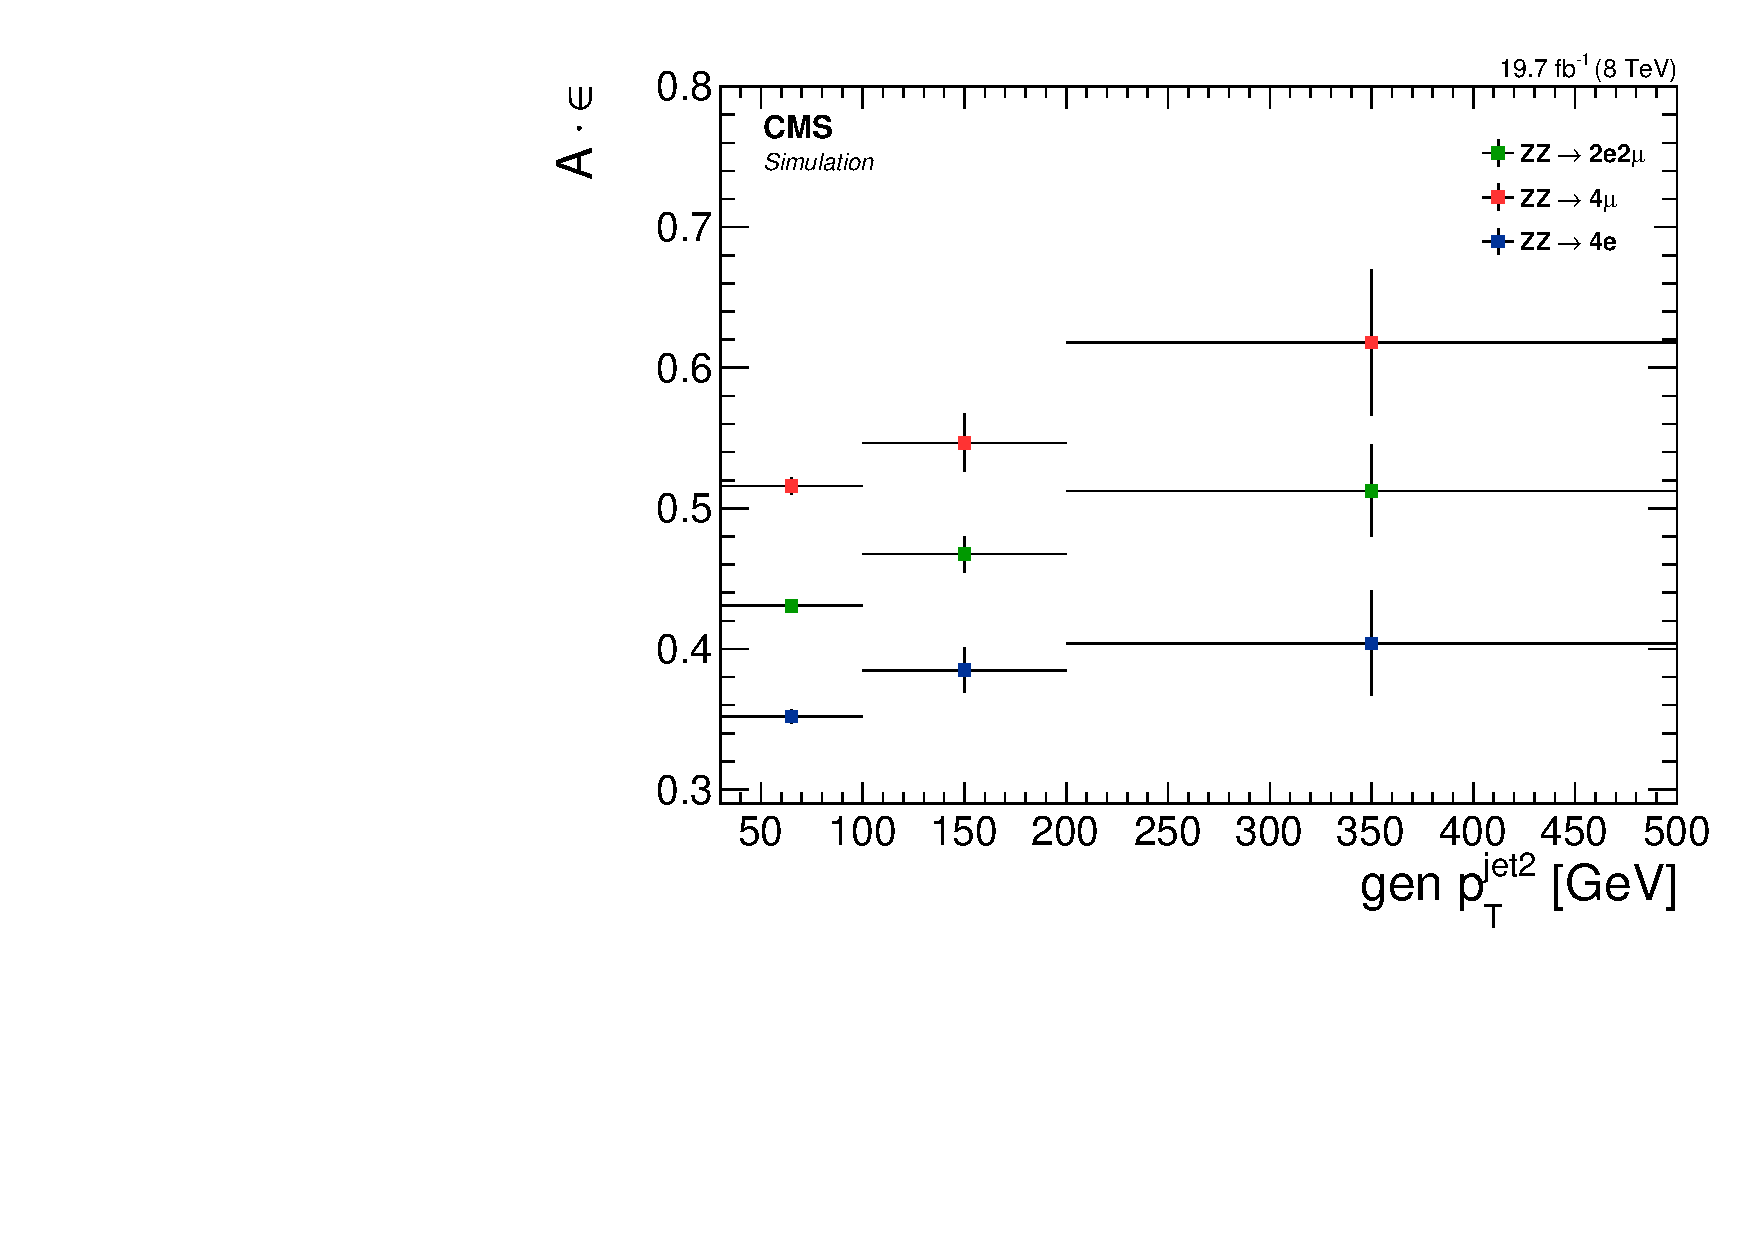
\includegraphics[width=\cmsFigWidth]{Figures/DiffAcceptance_PtJet2_Mad}
    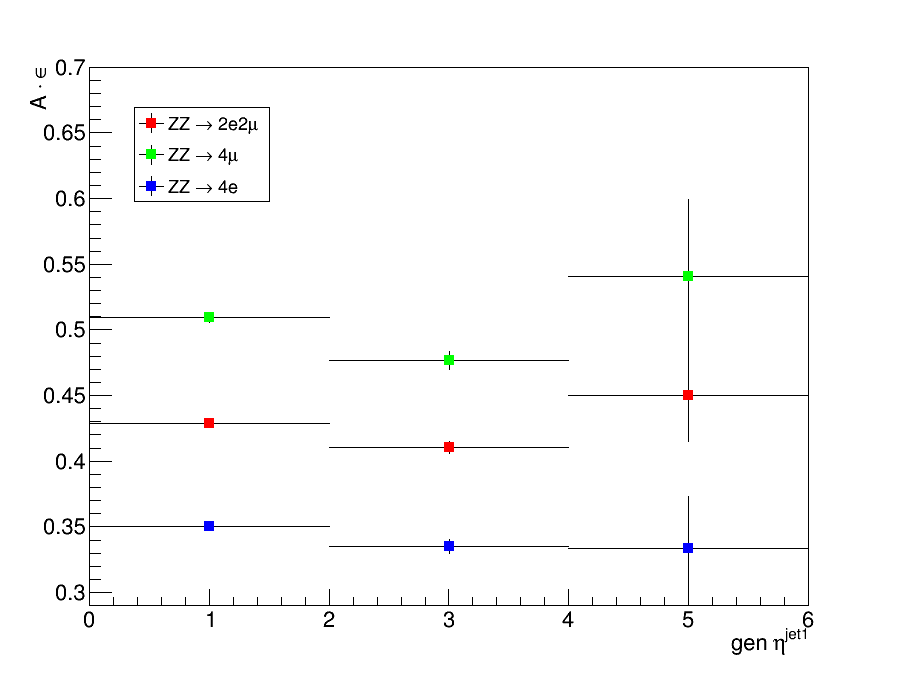
\includegraphics[width=\cmsFigWidth]{Figures/DiffAcceptance_EtaJet1_Mad}
    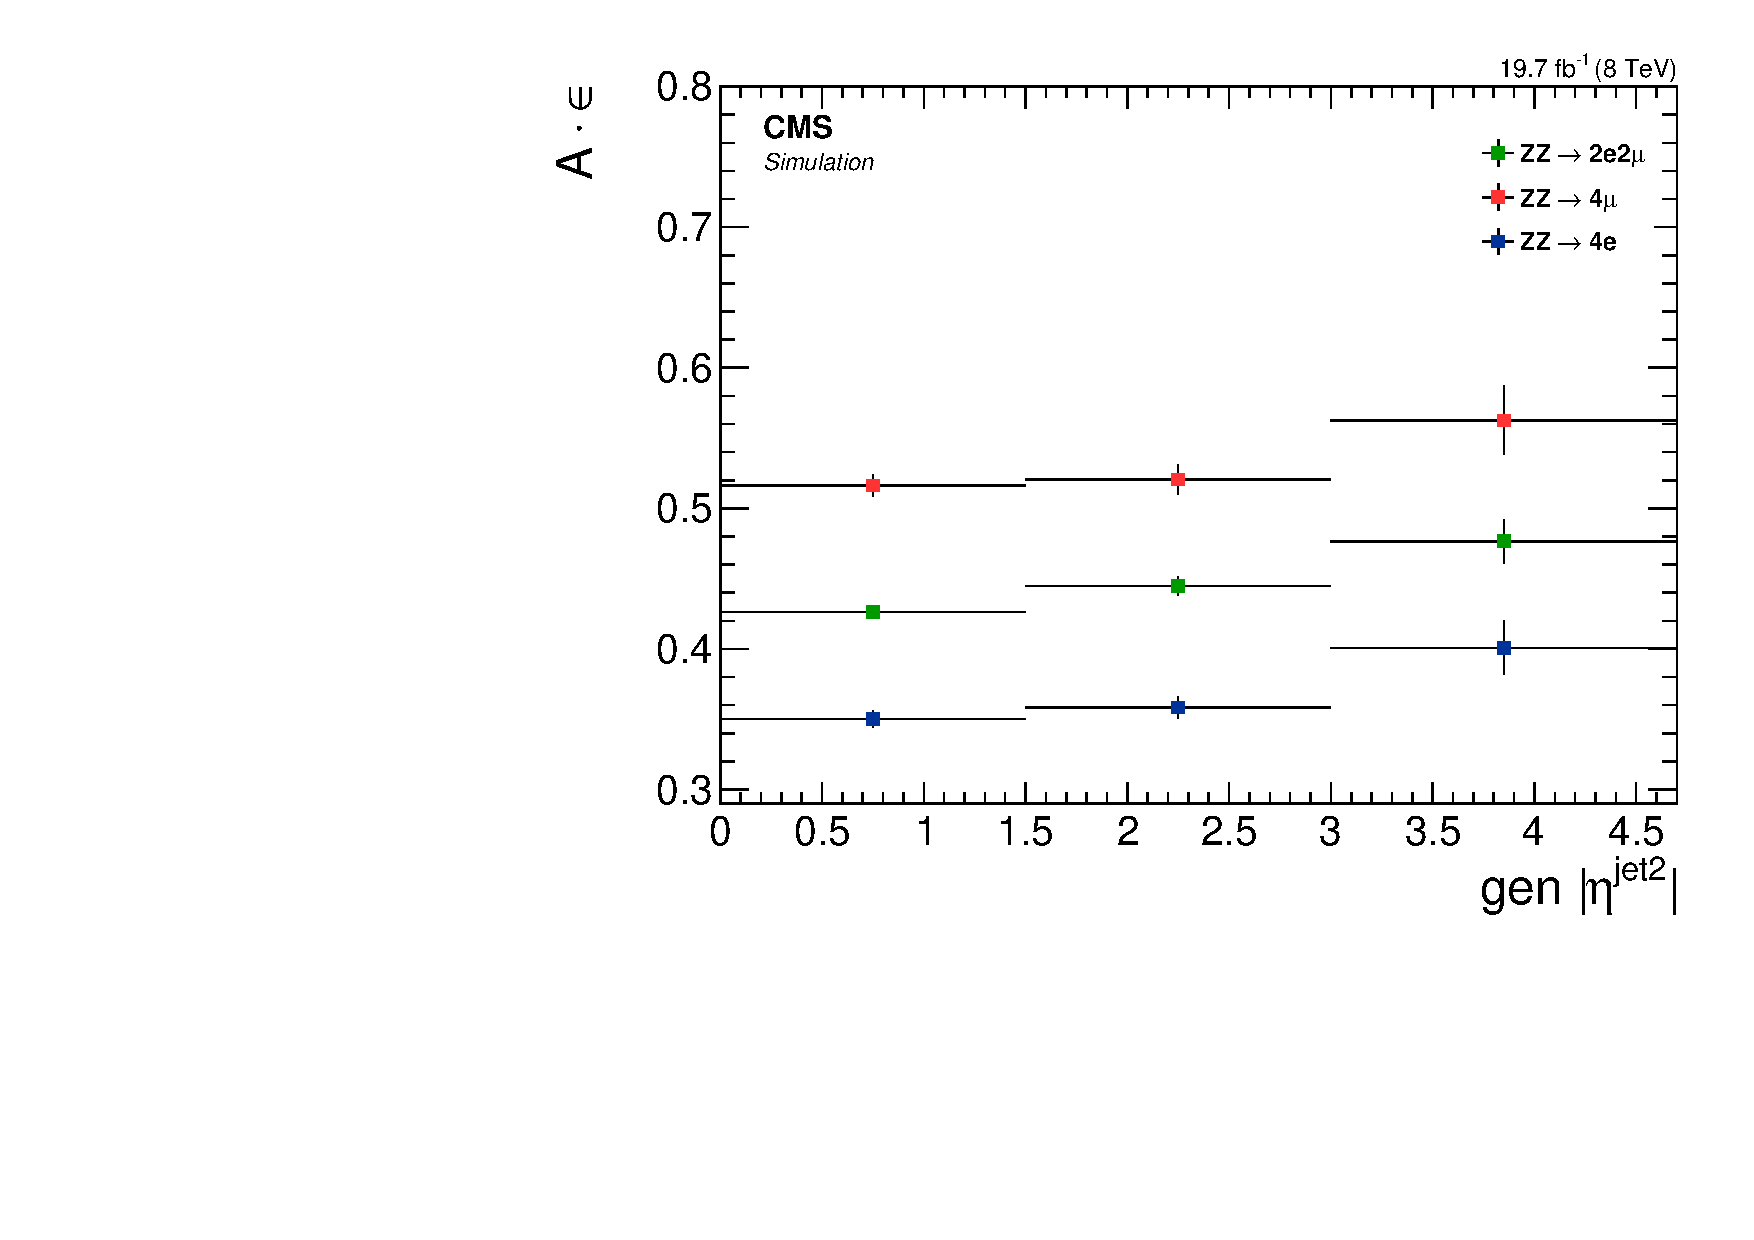
\includegraphics[width=\cmsFigWidth]{Figures/DiffAcceptance_EtaJet2_Mad}
    %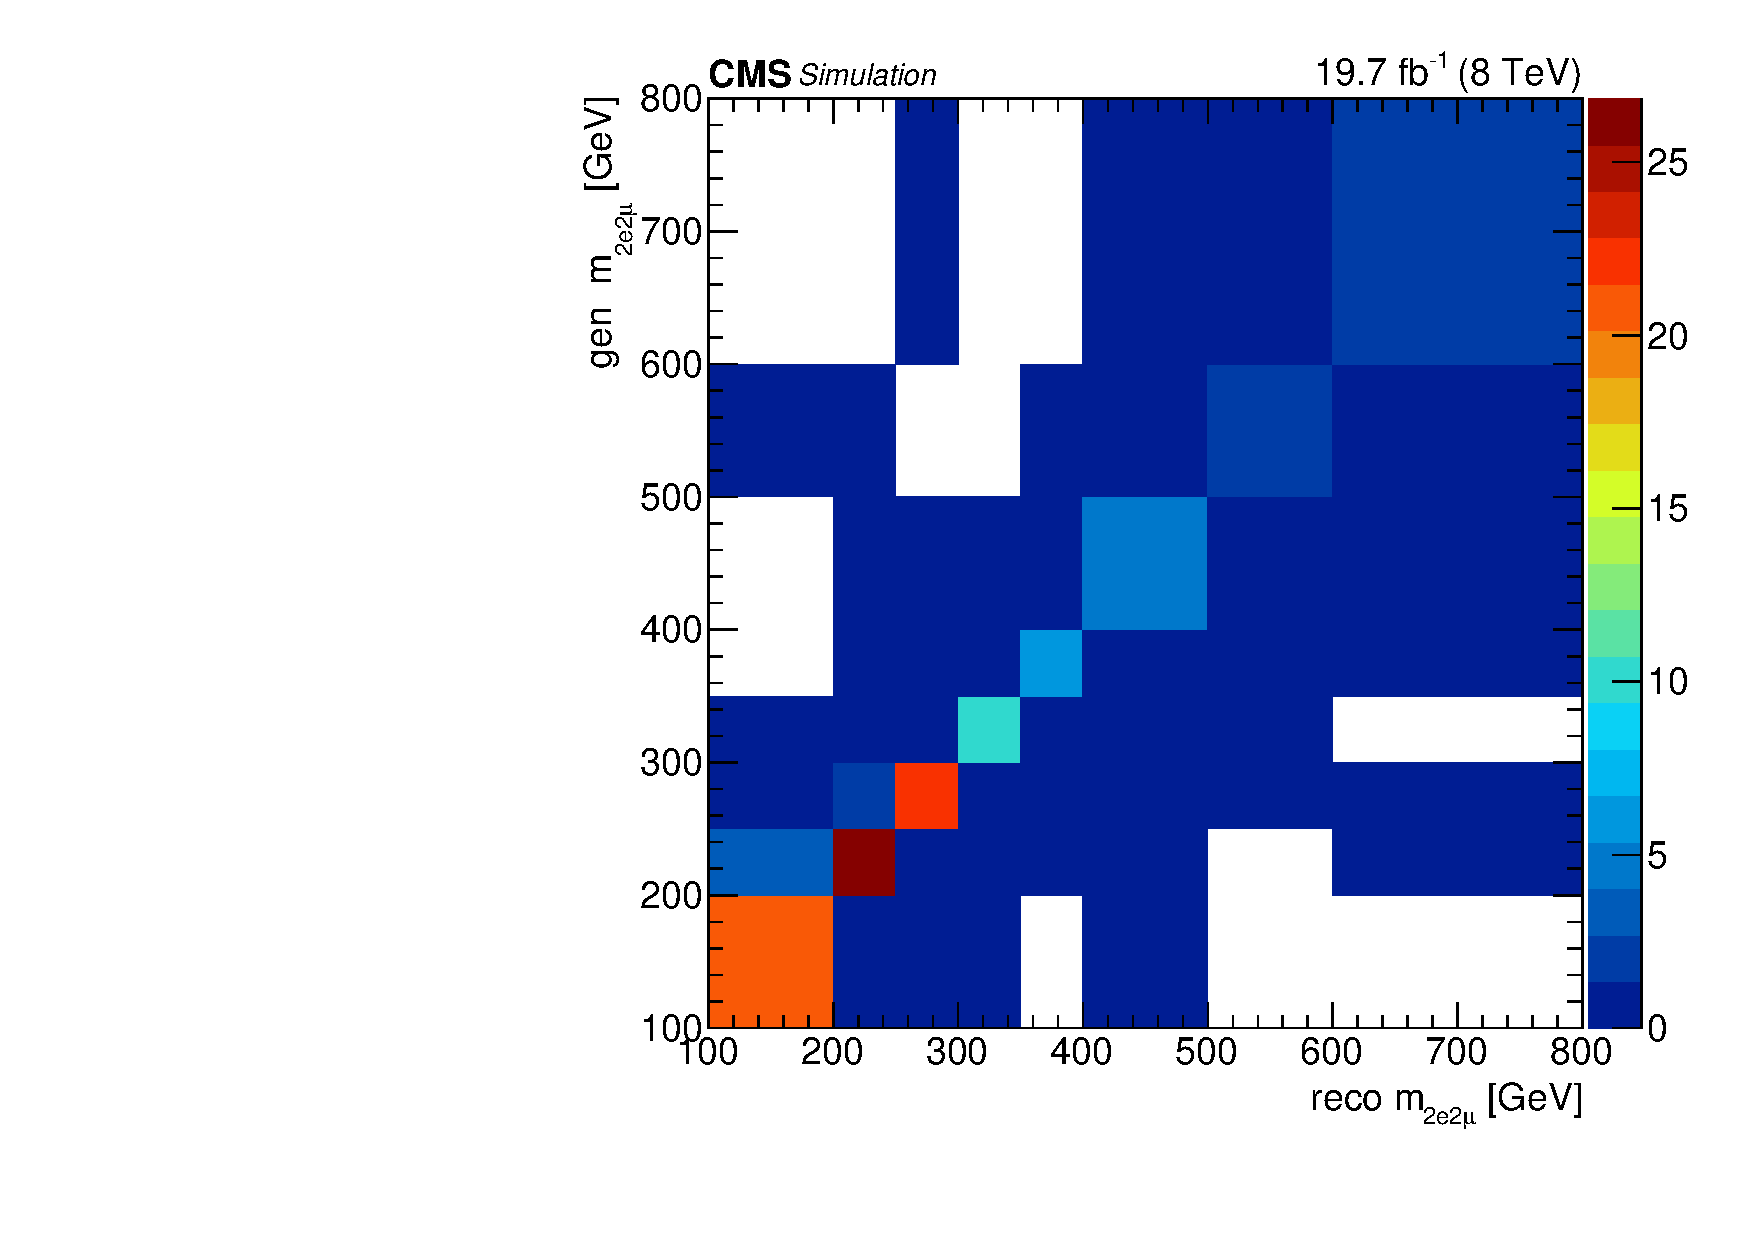
\includegraphics[width=\cmsFigWidth]{Figures/ResMat_qqggJJ_Mass_ZZTo2e2m_st_01_Pow}     
 %   to generate (a) and (b) labels under the figures, you can use subfloat, but this is not recommended: takes too much space
 %   \subfloat[]{
\includegraphics[width=0.2\textwidth]{CMS-bw-logo}}\subfloat[]{
\includegraphics[width=0.2\textwidth]{CMScol}}
    \caption{Acceptance ($A \cdot \epsilon$) computed in the wider fiducial region as a function of $p_T^{jet1}$  (top left), $p_T^{jet2}$  (top right), $\eta^{jet1}$ (bottom left) and $\eta^{jet2}$
distributions, according to the final state: 
      $4\mu$ (green), $4e$ (blue), $2e2\mu$  (red). Distributions are obtained using the  \texttt{Powheg} set of samples for  $m_{ZZ}$ and 
     the  \texttt{MadGraph} set of samples for the other variables.} 
    \label{fig:A_diff_jet}
  \end{center}
\end{figure}

\subsection{The differential ZZ cross-section measurements}
The study of vector boson pair production is important both as check of the SM and in search for new physics. 
Non-resonant $ZZ$ events are the dominant background in the $H \to ZZ \to 4\ell$ analysis and a good knowledge of 
these processes is  very useful for the study of the associated production of a $Z$ boson with the Higgs, especially at 13 TeV.
However, a lot of information
can still be extracted from data at 8 TeV, in particular as regards the associate production of a Z boson pair with jets. 
In addiction to the invariant mass of the four lepton system, the differential $ZZ$ cross-section is determined as
a function of the number of jets produced in the event, the invariant mass of the two most energetic jets ($m_{jj}$), the 
$\Delta\eta$ between them ($\Delta\eta_{jj}$), their transverse momentum and pseudorapidity (leading jet $p_{T}(\eta)^{jet1}$ and sub-leading jet $p_{T}(\eta)^{jet2}$). Both jets with  $\eta^{jet}<4.7$ and central jets with $\eta^{jet}<2.4$ are considered.\\
\\
The cross-section in each bin of each observable is determined from the event yields subtracting
the backgrounds. Each distribution is then corrected for event selection efficiencies
and for detector resolution effects in order to be compared with predictions from event generators.
The correction procedure is based on unfolding techniques, as implemented in the
\texttt{RooUnfold} toolkit~\cite{RooUnfold}, which provides both singular value decomposition (SVD)~\cite{SVD} and
the d'Agostini~\cite{DAgostini} methods. Both algorithms use a response matrix that correlates the observable
with and without detector effects. Regularization parameters can be tuned to obtain results that are robust against 
numerical instabilities and statistical fluctuations. The differential cross-section is then derived by dividing the
corrected number of events by the integrated luminosity, the branching ratio and the bin width.\\
\\
For each measured distribution, a response matrix is evaluated using two different sets of generators: the first one is composed of signal samples generated with \texttt{MadGraph} ($qq/qg/gg \to ZZ$), \texttt{MCFM} ($gg \to ZZ$) and \texttt{Phantom} ($qq \to ZZ+2jets$). The second one has the \texttt{Powheg} sample ($qq \to ZZ$) instead of
the \texttt{MadGraph} one. The \texttt{MadGraph} set is the reference set for the jet-related variables,
while the  \texttt{Powheg} one is used for check and comparison purposes. For the $m_{ZZ}$ distribution the role of the two sets of samples is switched.\\
As reported above, the signal definition of the generated events requires $60 < m_{Z_1}, m_{Z_2} < 120$  GeV. 
%  and $m_{ZZ} >$ 100 GeV. 
In order to minimize the model uncertainties due to unnecessary extrapolations of the measurement outside experimentally well-described phase space regions, cross-section distributions are also extracted in the tighter fiducial region, corresponding to the visible phase space defined by the kinematic and geometrical acceptance of leptons.\\ 
The same selection as in the inclusive cross-section measurement is applied to the reconstructed events.\\ 
Response matrices built using the reference set of samples and obtained in the tight fiducial region are 
reported in Figures~\ref{fig:Mass_matrices}-%,~\ref{fig:Jets_matrices},~\ref{fig:CentralJets_matrices},~\ref{fig:Mjj_matrices},~\ref{fig:Mjj_matrices},~\ref{fig:Deta_matrices},~\ref{fig:CentralDeta_matrices},~\ref{fig:PtJet1_matrices} and
\ref{fig:PtJet2_matrices} for each variable.\\
\begin{figure}[hbtp]
  \begin{center}
    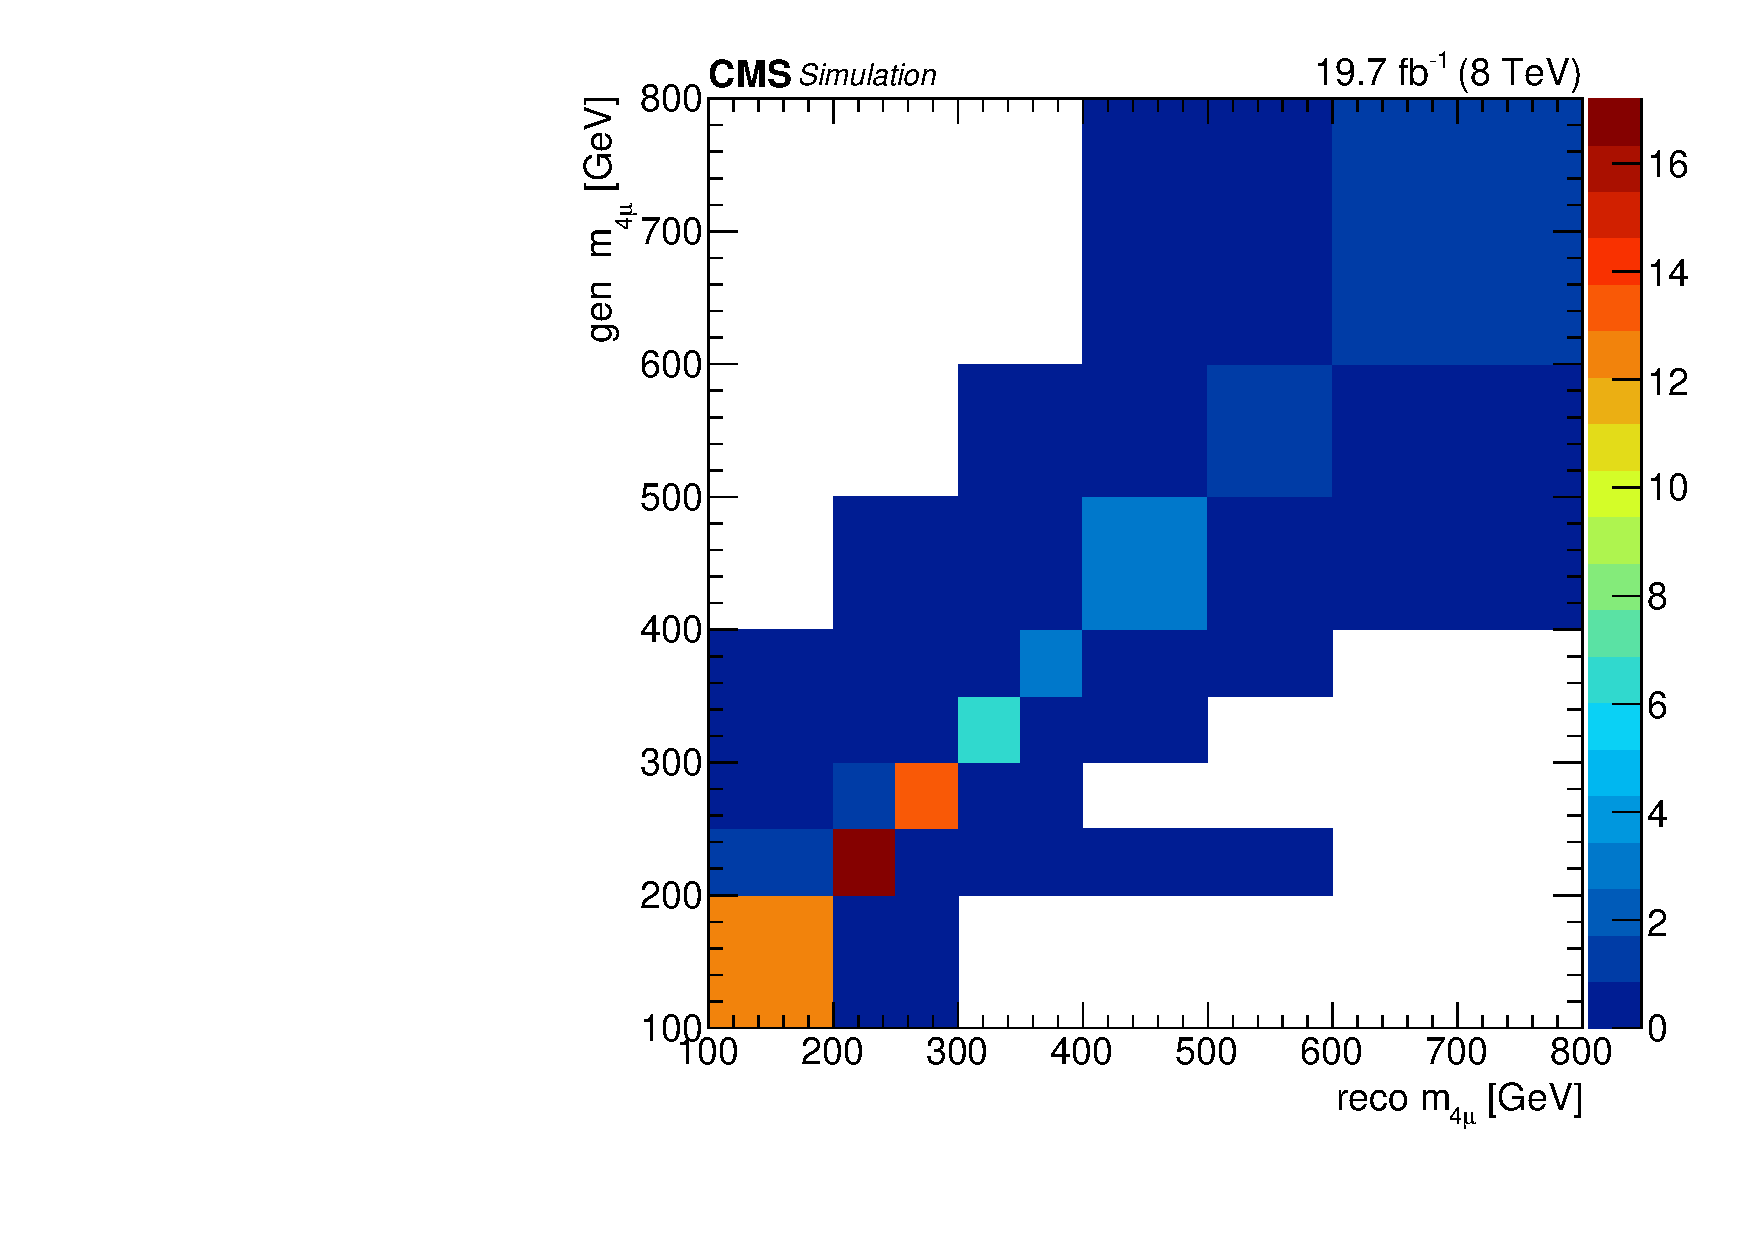
\includegraphics[width=\cmsFigWidth]{Figures/ResMat_qqggJJ_Mass_ZZTo4m_st_01_fr_Pow}
    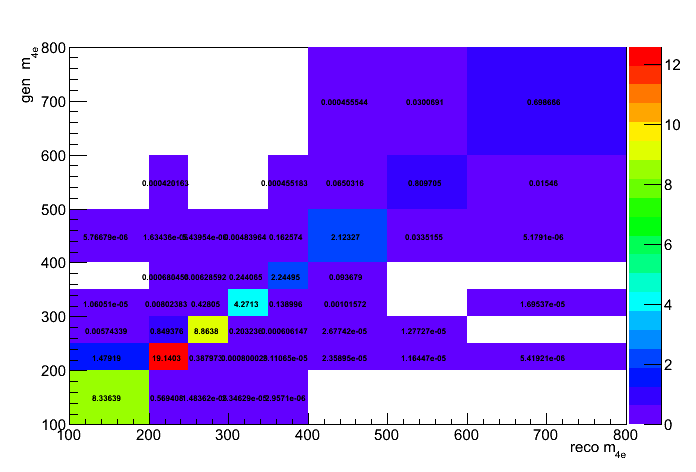
\includegraphics[width=\cmsFigWidth]{Figures/ResMat_qqggJJ_Mass_ZZTo4e_st_01_fr_Pow}
    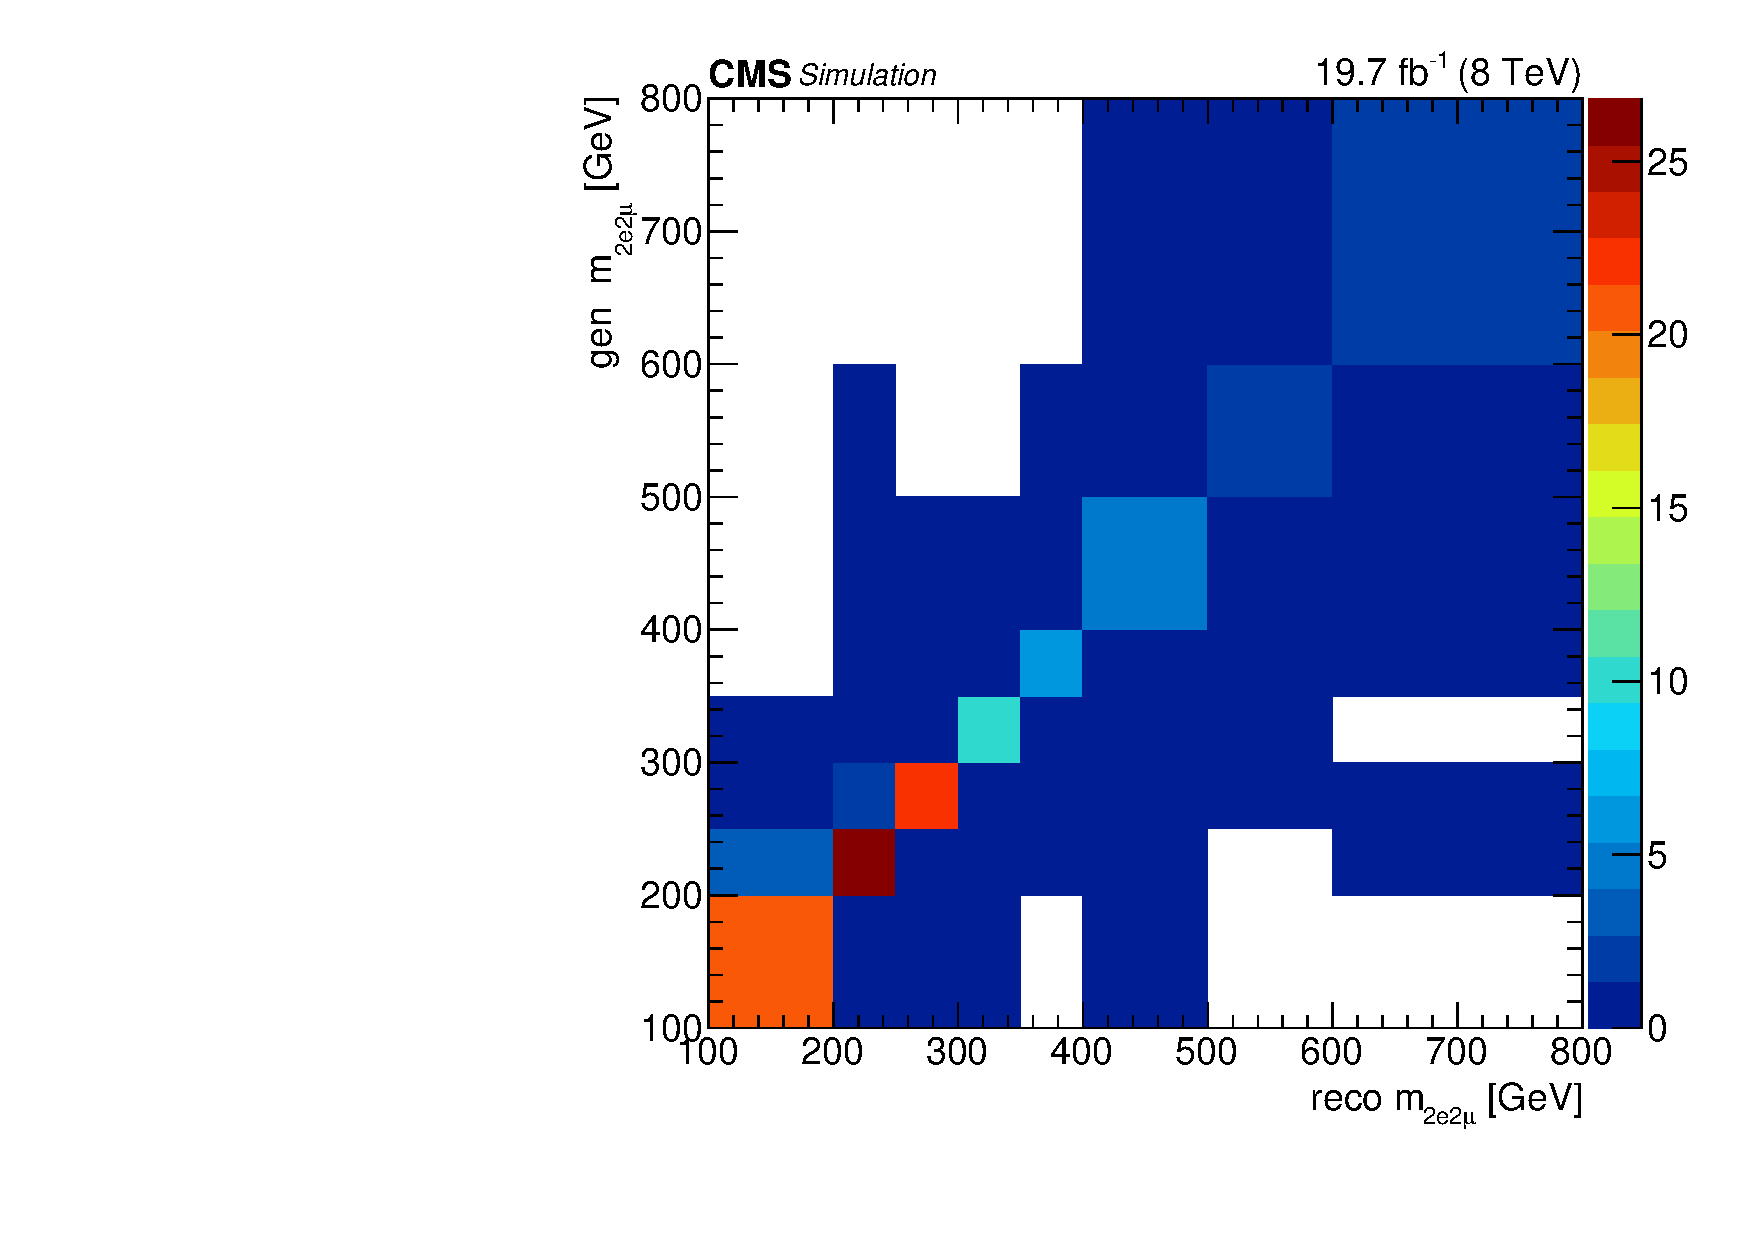
\includegraphics[width=\cmsFigWidth]{Figures/ResMat_qqggJJ_Mass_ZZTo2e2m_st_01_fr_Pow}     
 %   to generate (a) and (b) labels under the figures, you can use subfloat, but this is not recommended: takes too much space
 %   \subfloat[]{
\includegraphics[width=0.2\textwidth]{CMS-bw-logo}}\subfloat[]{
\includegraphics[width=0.2\textwidth]{CMScol}}
    \caption{Response matrices for the $m_{ZZ}$ distribution, according to the final state:  $4\mu$ (top left), $4e$ (top right), $2e2\mu$  (bottom). Matrices are obtained using the  \texttt{Powheg} set of samples. The tight fiducial region is considered.} 
    \label{fig:Mass_matrices}
  \end{center}
\end{figure}

\begin{figure}[hbtp]
  \begin{center}
    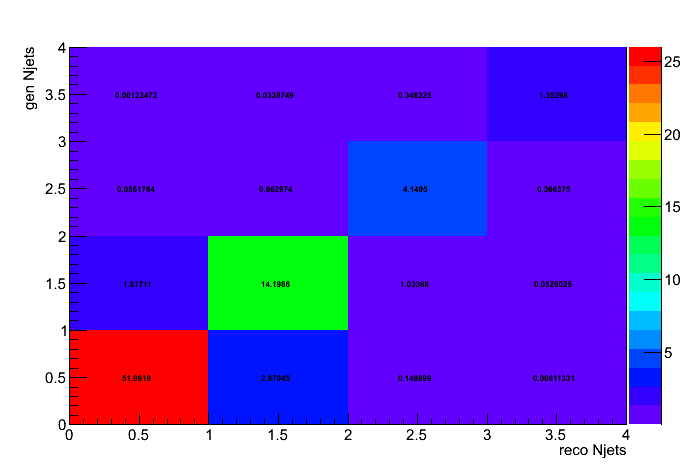
\includegraphics[width=\cmsFigWidth]{Figures/ResMat_qqggJJ_Jets_ZZTo4m_st_01_fr_Mad}
    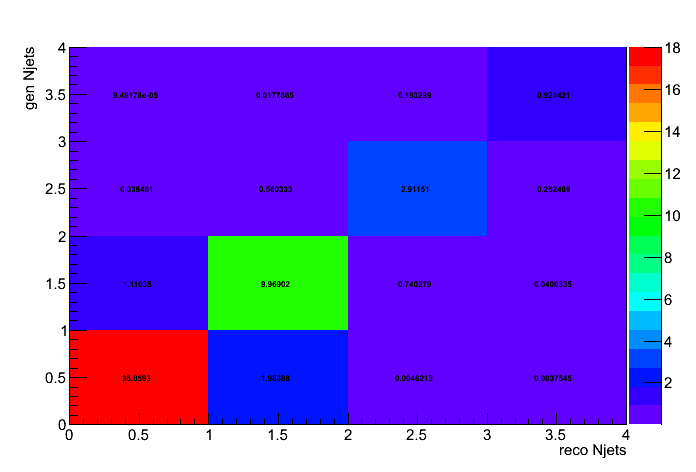
\includegraphics[width=\cmsFigWidth]{Figures/ResMat_qqggJJ_Jets_ZZTo4e_st_01_fr_Mad}
    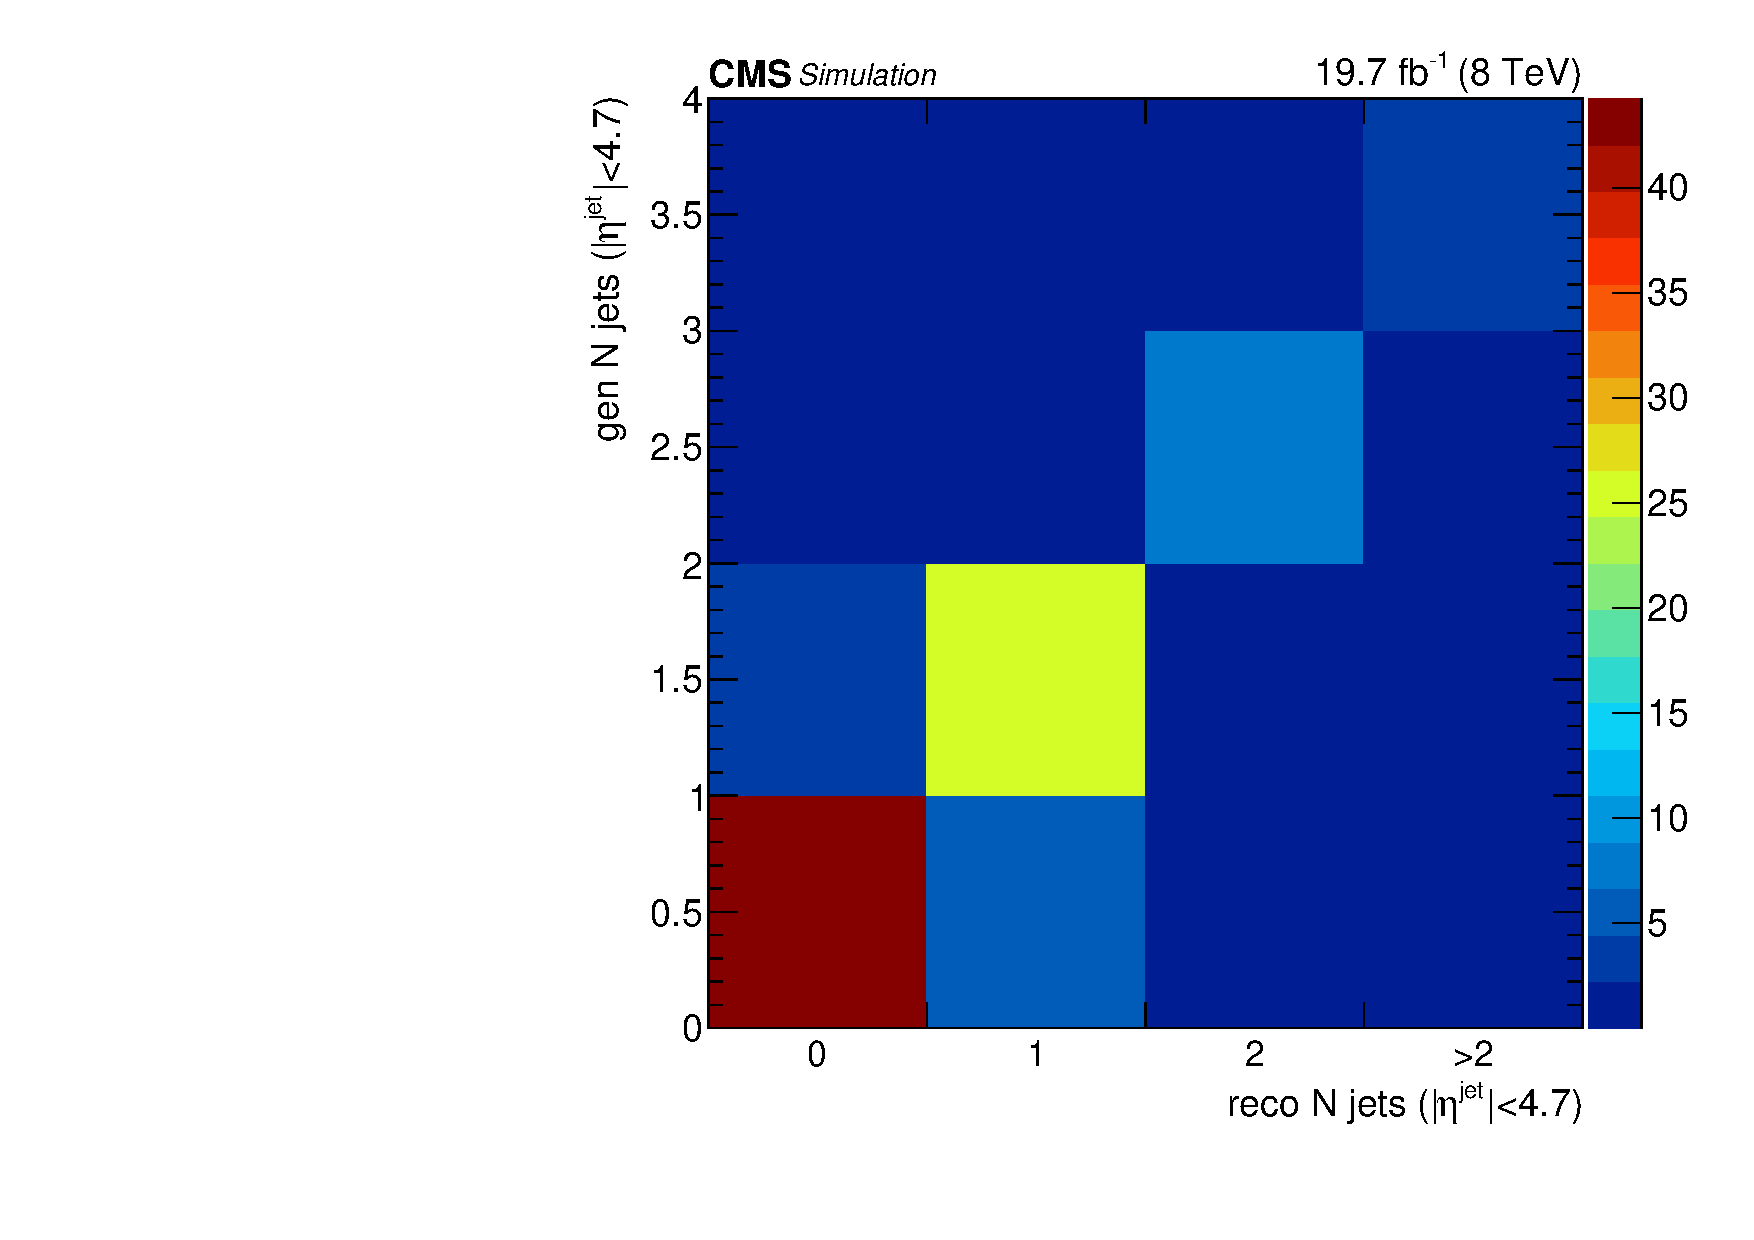
\includegraphics[width=\cmsFigWidth]{Figures/ResMat_qqggJJ_Jets_ZZTo2e2m_st_01_fr_Mad}     
 %   to generate (a) and (b) labels under the figures, you can use subfloat, but this is not recommended: takes too much space
 %   \subfloat[]{
\includegraphics[width=0.2\textwidth]{CMS-bw-logo}}\subfloat[]{
\includegraphics[width=0.2\textwidth]{CMScol}}
    \caption{Response matrices for the $N\ jets$ distribution, according to the final state:  $4\mu$ (top left), $4e$ (top right), $2e2\mu$  (bottom). Matrices are obtained using the  \texttt{MadGraph} set of samples. The tight fiducial region is considered.} 
    \label{fig:Jets_matrices}
  \end{center}
\end{figure}
\begin{figure}[hbtp]
  \begin{center}
    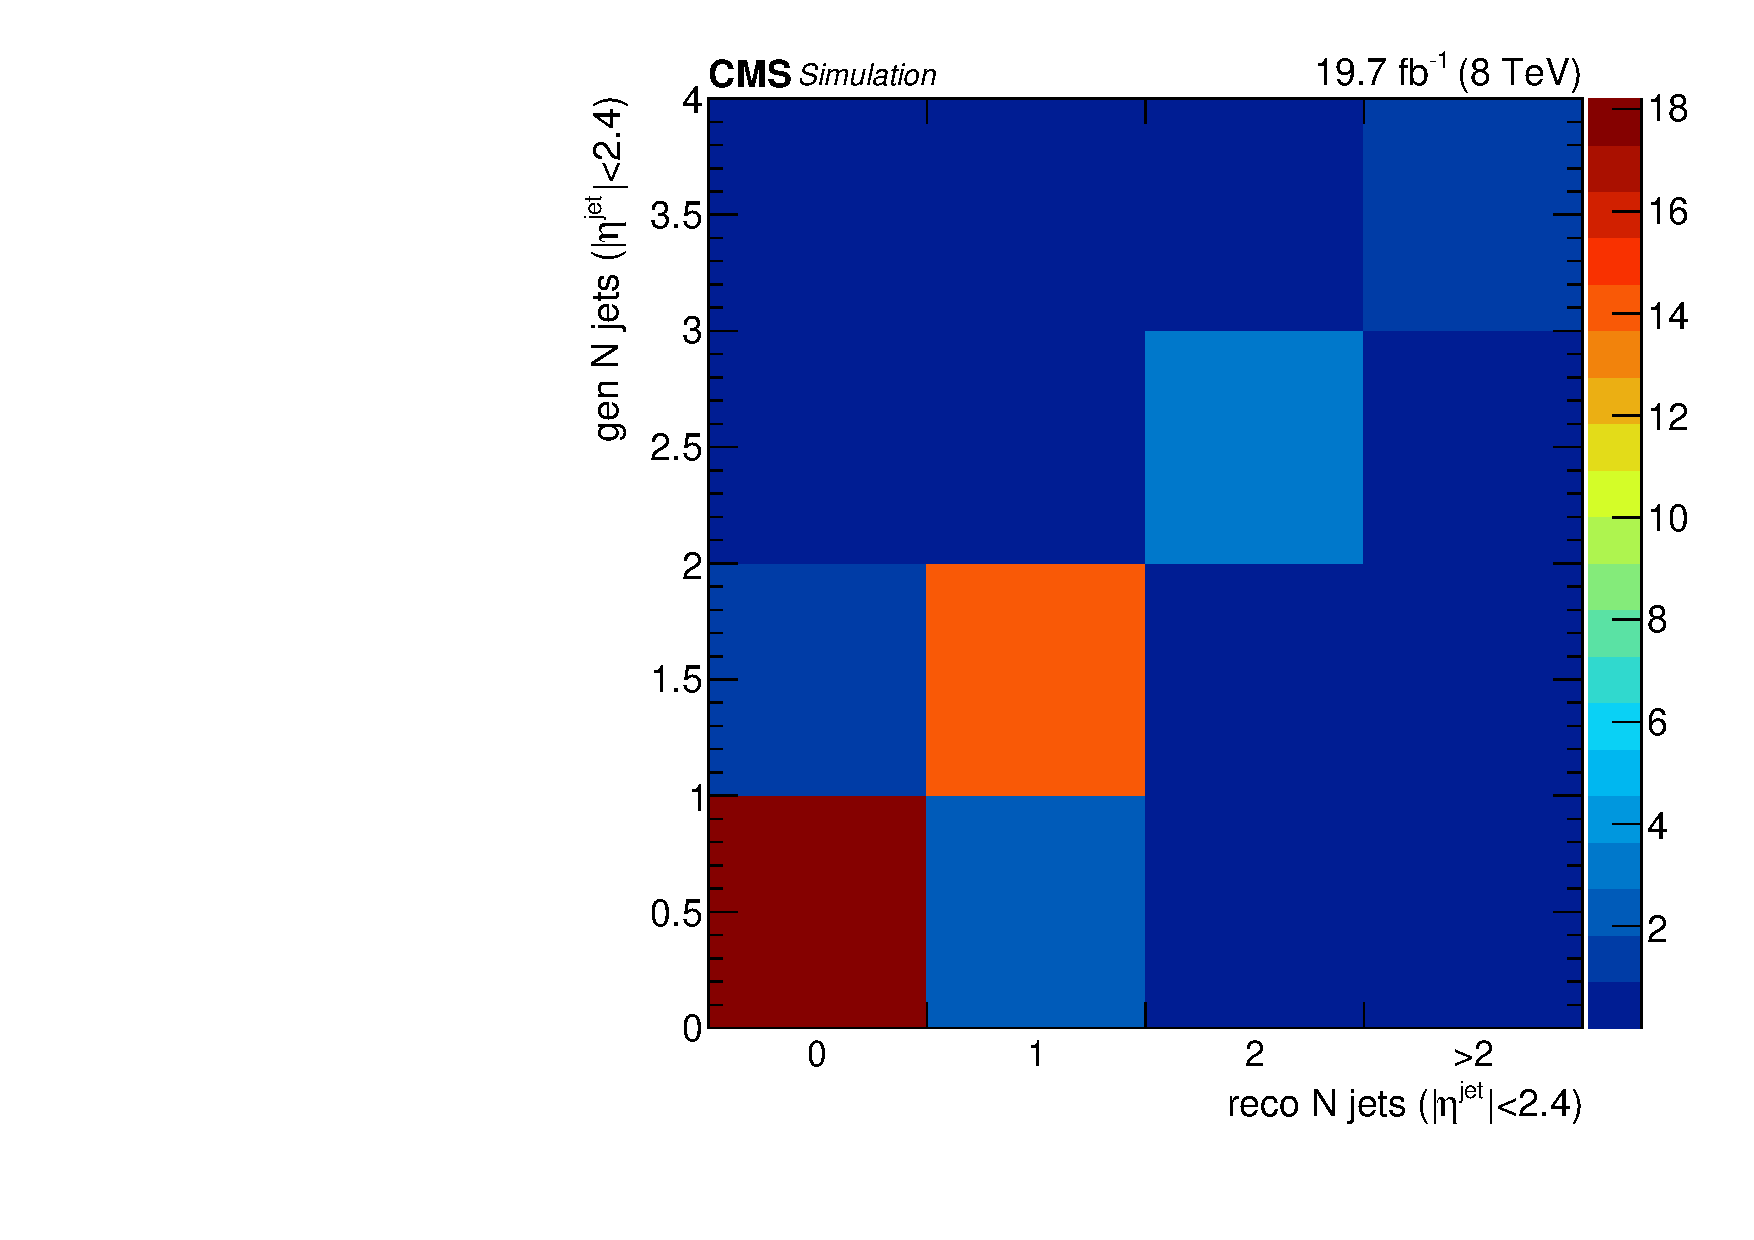
\includegraphics[width=\cmsFigWidth]{Figures/ResMat_qqggJJ_CentralJets_ZZTo4m_st_01_fr_Mad}
    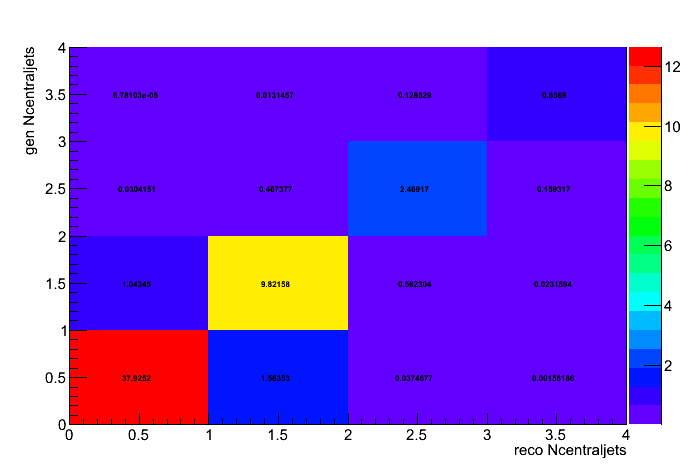
\includegraphics[width=\cmsFigWidth]{Figures/ResMat_qqggJJ_CentralJets_ZZTo4e_st_01_fr_Mad}
    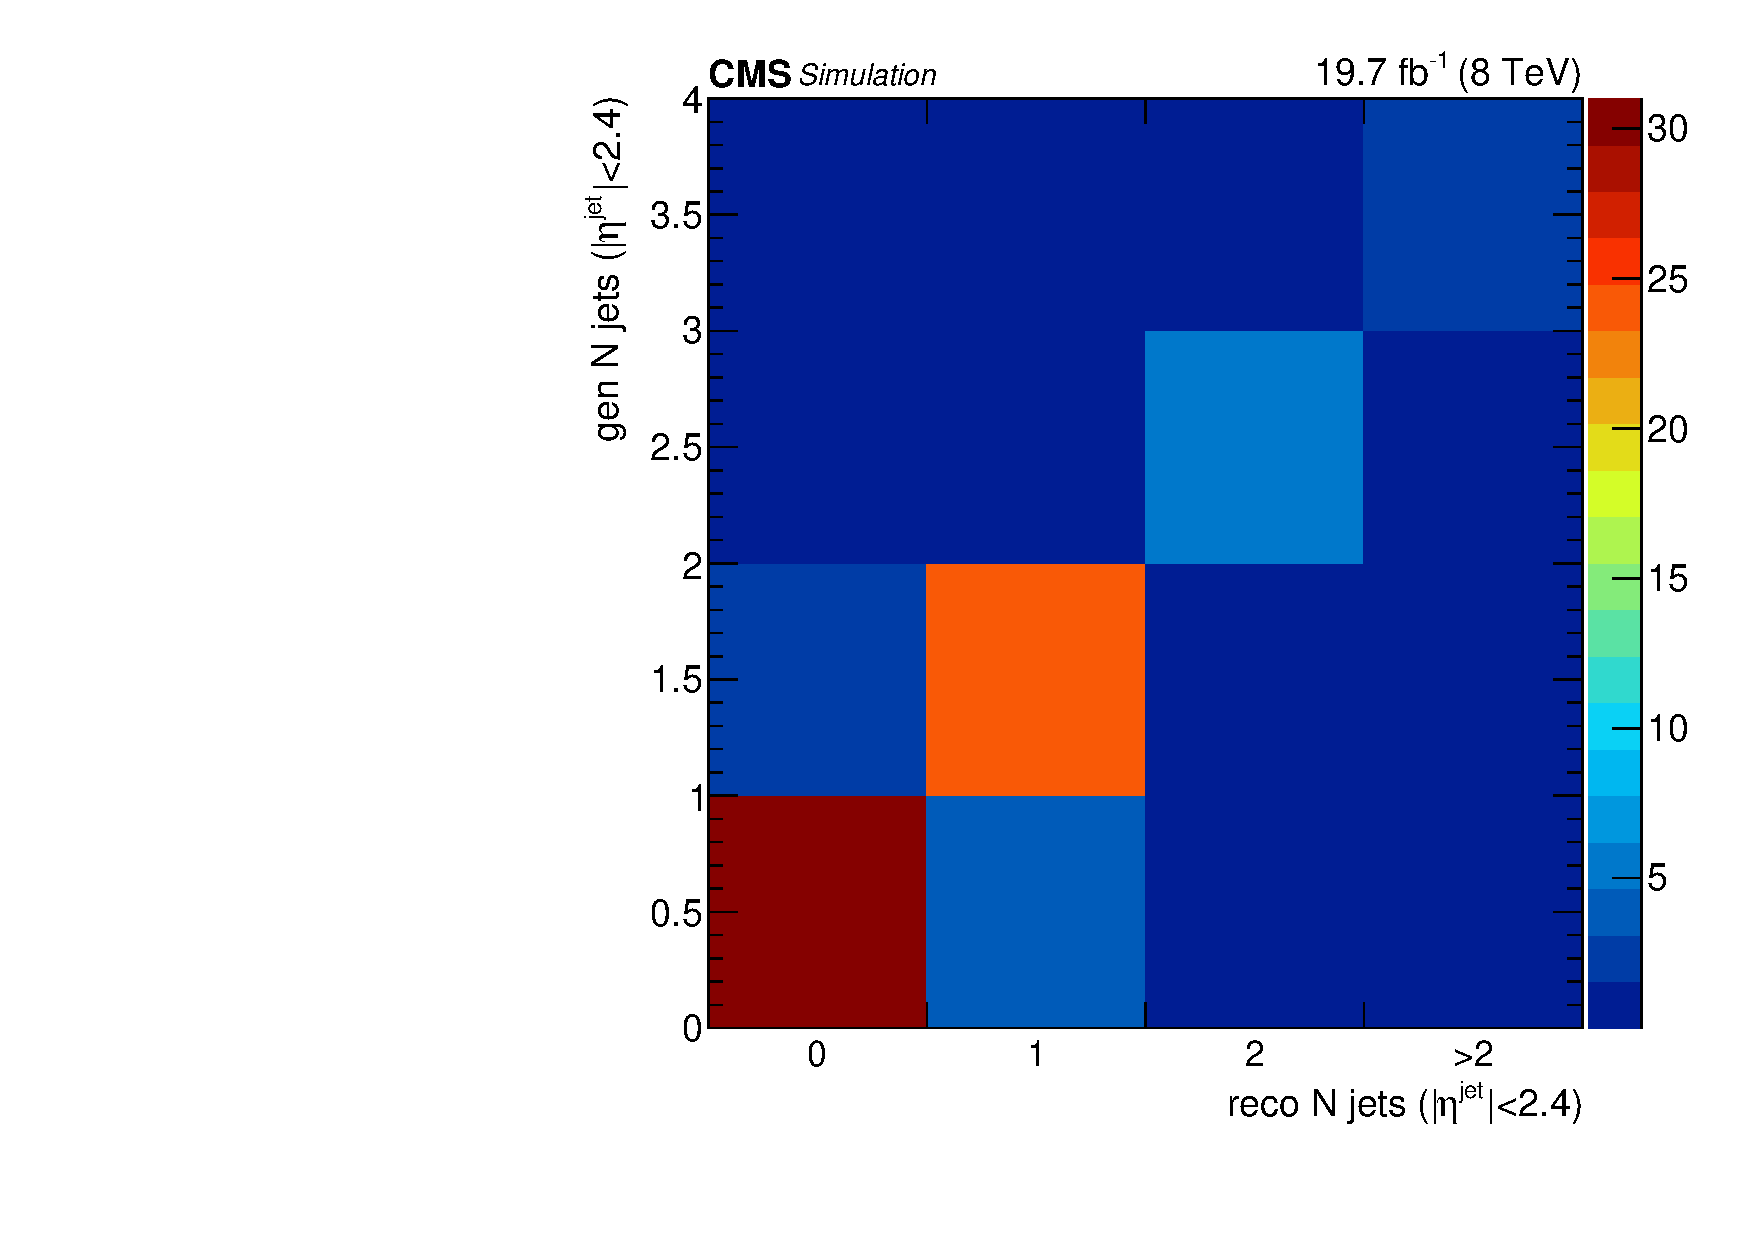
\includegraphics[width=\cmsFigWidth]{Figures/ResMat_qqggJJ_CentralJets_ZZTo2e2m_st_01_fr_Mad}     
 %   to generate (a) and (b) labels under the figures, you can use subfloat, but this is not recommended: takes too much space
 %   \subfloat[]{
\includegraphics[width=0.2\textwidth]{CMS-bw-logo}}\subfloat[]{
\includegraphics[width=0.2\textwidth]{CMScol}}
    \caption{Response matrices for the $N\ central\ jets$ distribution (with $\eta^{jet}<2.4$) , according to the final state:  $4\mu$ (top left), $4e$ (top right), $2e2\mu$  (bottom). Matrices are obtained using the  \texttt{MadGraph} set of samples. The tight fiducial region is considered.} 
    \label{fig:CentralJets_matrices}
  \end{center}
\end{figure}
\begin{figure}[hbtp]
  \begin{center}
    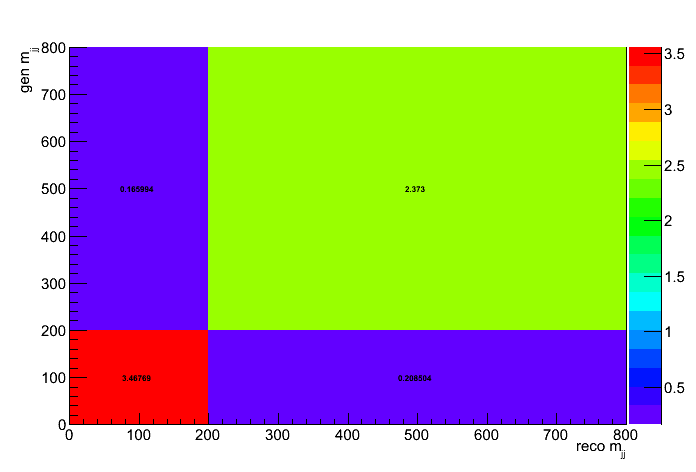
\includegraphics[width=\cmsFigWidth]{Figures/ResMat_qqggJJ_Mjj_ZZTo4m_st_01_fr_Mad}
    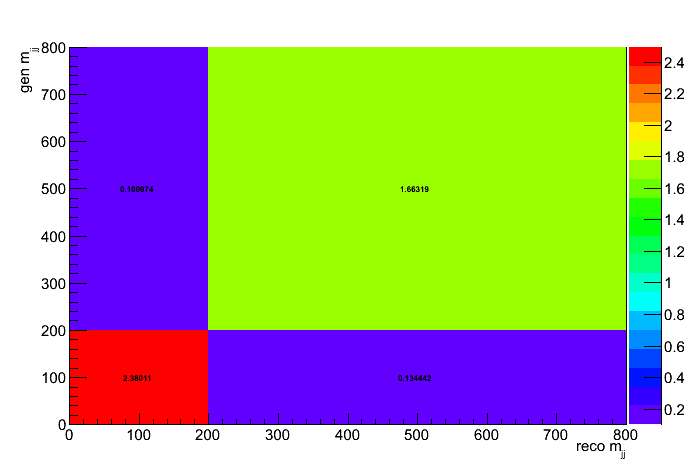
\includegraphics[width=\cmsFigWidth]{Figures/ResMat_qqggJJ_Mjj_ZZTo4e_st_01_fr_Mad}
    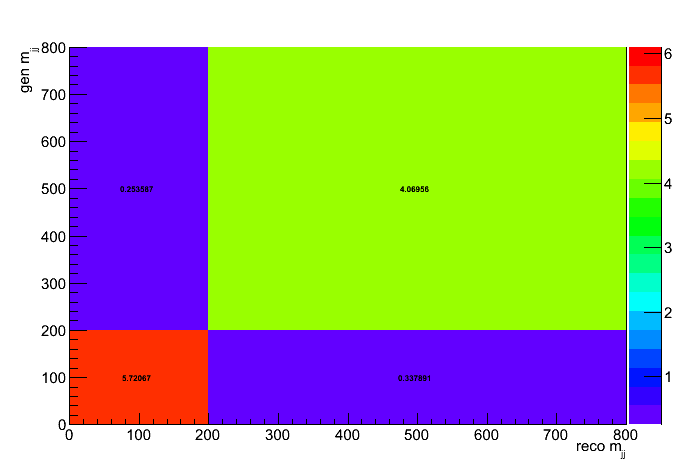
\includegraphics[width=\cmsFigWidth]{Figures/ResMat_qqggJJ_Mjj_ZZTo2e2m_st_01_fr_Mad}     
 %   to generate (a) and (b) labels under the figures, you can use subfloat, but this is not recommended: takes too much space
 %   \subfloat[]{
\includegraphics[width=0.2\textwidth]{CMS-bw-logo}}\subfloat[]{\includegraphics[width=0.2\textwidth]{CMScol}}
    \caption{Response matrices for the $m_{jj}$ distribution, according to the final state:  $4\mu$ (top left), $4e$ (top right), $2e2\mu$  (bottom). Matrices are obtained using the  \texttt{MadGraph} set of samples. The tight fiducial region is considered.} 
    \label{fig:Mjj_matrices}
  \end{center}
\end{figure}
\begin{figure}[hbtp]
  \begin{center}
    \includegraphics[width=\cmsFigWidth]{Figures/ResMat_qqggJJ_CentralMjj_ZZTo4m_st_01_fr_Mad}
    \includegraphics[width=\cmsFigWidth]{Figures/ResMat_qqggJJ_CentralMjj_ZZTo4e_st_01_fr_Mad}
    \includegraphics[width=\cmsFigWidth]{Figures/ResMat_qqggJJ_CentralMjj_ZZTo2e2m_st_01_fr_Mad}     
 %   to generate (a) and (b) labels under the figures, you can use subfloat, but this is not recommended: takes too much space
 %   \subfloat[]{\includegraphics[width=0.2\textwidth]{CMS-bw-logo}}\subfloat[]{\includegraphics[width=0.2\textwidth]{CMScol}}
    \caption{Response matrices for the $m_{jj}$ distribution (with $\eta^{jet}<2.4$), according to the final state:  $4\mu$ (top left), $4e$ (top right), $2e2\mu$  (bottom). Matrices are obtained using the  \texttt{MadGraph} set of samples. The tight fiducial region is considered.} 
    \label{fig:CentralMjj_matrices}
  \end{center}
\end{figure}
\begin{figure}[hbtp]
  \begin{center}
    \includegraphics[width=\cmsFigWidth]{Figures/ResMat_qqggJJ_Deta_ZZTo4m_st_01_fr_Mad}
    \includegraphics[width=\cmsFigWidth]{Figures/ResMat_qqggJJ_Deta_ZZTo4e_st_01_fr_Mad}
    \includegraphics[width=\cmsFigWidth]{Figures/ResMat_qqggJJ_Deta_ZZTo2e2m_st_01_fr_Mad}     
 %   to generate (a) and (b) labels under the figures, you can use subfloat, but this is not recommended: takes too much space
 %   \subfloat[]{\includegraphics[width=0.2\textwidth]{CMS-bw-logo}}\subfloat[]{\includegraphics[width=0.2\textwidth]{CMScol}}
    \caption{Response matrices for the $\Delta\eta_{jj}$ distribution, according to the final state:  $4\mu$ (top left), $4e$ (top right), $2e2\mu$  (bottom). Matrices are obtained using the  \texttt{MadGraph} set of samples. The tight fiducial region is considered.} 
    \label{fig:Deta_matrices}
  \end{center}
\end{figure}
\begin{figure}[hbtp]
  \begin{center}
    \includegraphics[width=\cmsFigWidth]{Figures/ResMat_qqggJJ_CentralDeta_ZZTo4m_st_01_fr_Mad}
    \includegraphics[width=\cmsFigWidth]{Figures/ResMat_qqggJJ_CentralDeta_ZZTo4e_st_01_fr_Mad}
    \includegraphics[width=\cmsFigWidth]{Figures/ResMat_qqggJJ_CentralDeta_ZZTo2e2m_st_01_fr_Mad}     
 %   to generate (a) and (b) labels under the figures, you can use subfloat, but this is not recommended: takes too much space
 %   \subfloat[]{\includegraphics[width=0.2\textwidth]{CMS-bw-logo}}\subfloat[]{\includegraphics[width=0.2\textwidth]{CMScol}}
    \caption{Response matrices for the $\Delta\eta_{jj}$ distribution (with $\eta^{jet}<2.4$), according to the final state:  $4\mu$ (top left), $4e$ (top right), $2e2\mu$  (bottom). Matrices are obtained using the  \texttt{MadGraph} set of samples. The tight fiducial region is considered.} 
    \label{fig:CentralDeta_matrices}
  \end{center}
\end{figure}
\begin{figure}[hbtp]
  \begin{center}
    \includegraphics[width=\cmsFigWidth]{Figures/ResMat_qqggJJ_PtJet1_ZZTo4m_st_01_fr_Mad}
    \includegraphics[width=\cmsFigWidth]{Figures/ResMat_qqggJJ_PtJet1_ZZTo4e_st_01_fr_Mad}
    \includegraphics[width=\cmsFigWidth]{Figures/ResMat_qqggJJ_PtJet1_ZZTo2e2m_st_01_fr_Mad}     
 %   to generate (a) and (b) labels under the figures, you can use subfloat, but this is not recommended: takes too much space
 %   \subfloat[]{\includegraphics[width=0.2\textwidth]{CMS-bw-logo}}\subfloat[]{\includegraphics[width=0.2\textwidth]{CMScol}}
    \caption{Response matrices for the $p_{T}$ distribution of the leading jet, according to the final state:  $4\mu$ (top left), $4e$ (top right), $2e2\mu$  (bottom). Matrices are obtained using the  \texttt{MadGraph} set of samples. The tight fiducial region is considered. } 
    \label{fig:PtJet1_matrices}
  \end{center}
\end{figure}
\begin{figure}[hbtp]
  \begin{center}
    \includegraphics[width=\cmsFigWidth]{Figures/ResMat_qqggJJ_PtJet2_ZZTo4m_st_01_fr_Mad}
    \includegraphics[width=\cmsFigWidth]{Figures/ResMat_qqggJJ_PtJet2_ZZTo4e_st_01_fr_Mad}
    \includegraphics[width=\cmsFigWidth]{Figures/ResMat_qqggJJ_PtJet2_ZZTo2e2m_st_01_fr_Mad}     
 %   to generate (a) and (b) labels under the figures, you can use subfloat, but this is not recommended: takes too much space
 %   \subfloat[]{\includegraphics[width=0.2\textwidth]{CMS-bw-logo}}\subfloat[]{\includegraphics[width=0.2\textwidth]{CMScol}}
    \caption{Response matrices for the $p_{T}$ distribution of the sub-leading jet, according to the final state:  $4\mu$ (top left), $4e$ (top right), $2e2\mu$  (bottom). Matrices are obtained using the  \texttt{MadGraph} set of samples. The tight fiducial region is considered.} 
    \label{fig:PtJet2_matrices}
  \end{center}
\end{figure}

\begin{figure}[hbtp]
  \begin{center}
    \includegraphics[width=\cmsFigWidth]{Figures/ResMat_qqggJJ_EtaJet1_ZZTo4m_st_01_fr_Mad}
    \includegraphics[width=\cmsFigWidth]{Figures/ResMat_qqggJJ_EtaJet1_ZZTo4e_st_01_fr_Mad}
    \includegraphics[width=\cmsFigWidth]{Figures/ResMat_qqggJJ_EtaJet1_ZZTo2e2m_st_01_fr_Mad}     
 %   to generate (a) and (b) labels under the figures, you can use subfloat, but this is not recommended: takes too much space
 %   \subfloat[]{\includegraphics[width=0.2\textwidth]{CMS-bw-logo}}\subfloat[]{\includegraphics[width=0.2\textwidth]{CMScol}}
    \caption{Response matrices for the $\eta$ distribution of the leading jet, according to the final state:  $4\mu$ (top left), $4e$ (top right), $2e2\mu$  (bottom). Matrices are obtained using the  \texttt{MadGraph} set of samples. The tight fiducial region is considered.} 
    \label{fig:EtaJet1_matrices}
  \end{center}
\end{figure}
\begin{figure}[hbtp]
  \begin{center}
    \includegraphics[width=\cmsFigWidth]{Figures/ResMat_qqggJJ_EtaJet2_ZZTo4m_st_01_fr_Mad}
    \includegraphics[width=\cmsFigWidth]{Figures/ResMat_qqggJJ_EtaJet2_ZZTo4e_st_01_fr_Mad}
    \includegraphics[width=\cmsFigWidth]{Figures/ResMat_qqggJJ_EtaJet2_ZZTo2e2m_st_01_fr_Mad}     
 %   to generate (a) and (b) labels under the figures, you can use subfloat, but this is not recommended: takes too much space
 %   \subfloat[]{\includegraphics[width=0.2\textwidth]{CMS-bw-logo}}\subfloat[]{\includegraphics[width=0.2\textwidth]{CMScol}}
    \caption{Response matrices for the $\eta$ distribution of the sub-leading jet, according to the final state:  $4\mu$ (top left), $4e$ (top right), $2e2\mu$  (bottom). Matrices are obtained using the  \texttt{MadGraph} set of samples. The tight fiducial region is considered.} 
    \label{fig:EtaJet2_matrices}
  \end{center}
\end{figure}
\clearpage

\begin{figure}[hbtp]
  \begin{center}
    \includegraphics[width=\cmsFigWidth]{Figures/Mass_ZZTo4m_Pow_fr_binwidth}
    \includegraphics[width=\cmsFigWidth]{Figures/Mass_ZZTo4e_Pow_fr_binwidth}
    \includegraphics[width=\cmsFigWidth]{Figures/Mass_ZZTo2e2m_Pow_fr_binwidth}  
    \includegraphics[width=\cmsFigWidth]{Figures/Mass_ZZTo4l_Pow_fr}    
 %   to generate (a) and (b) labels under the figures, you can use subfloat, but this is not recommended: takes too much space
 %   \subfloat[]{\includegraphics[width=0.2\textwidth]{CMS-bw-logo}}\subfloat[]{\includegraphics[width=0.2\textwidth]{CMScol}}
    \caption{\footnotesize{Data (red), unfolded data (blue), generated (dashed blue) and MC reconstructed (dashed red) $m_{ZZ}$ distributions, according to the final state: 
$4\mu$ (top left), $4e$ (top right), $2e2\mu$  (bottom left),  $4\ell$ (bottom right). The unfolded distributions are obtained  in the tight fiducial region using the SVD algorithm, with $k_{reg} = 4$, and compared to predictions from the \texttt{Powheg} set of samples.}} 
    \label{fig:Mass_unfolding}
  \end{center}
\end{figure}

\begin{figure}[hbtp]
  \begin{center}
    \includegraphics[width=\cmsFigWidth]{Figures/Jets_ZZTo4m_Mad_fr_binwidth}
    \includegraphics[width=\cmsFigWidth]{Figures/Jets_ZZTo4e_Mad_fr_binwidth}
    \includegraphics[width=\cmsFigWidth]{Figures/Jets_ZZTo2e2m_Mad_fr_binwidth}     
    \includegraphics[width=\cmsFigWidth]{Figures/Jets_ZZTo4l_Mad_fr}    
 %   to generate (a) and (b) labels under the figures, you can use subfloat, but this is not recommended: takes too much space
 %   \subfloat[]{\includegraphics[width=0.2\textwidth]{CMS-bw-logo}}\subfloat[]{\includegraphics[width=0.2\textwidth]{CMScol}}
    \caption{\footnotesize{Data (red), unfolded data (blue), generated (dashed blue) and MC reconstructed (dashed red) $N\ jets$ distributions, according to the final state: (top left) $4\mu$, (top right) $4e$, (bottom left) $2e2\mu$, (bottom right) $4\ell$. The unfolded distributions are obtained in the tight fiducial region using the D'Agostini algorithm, with 4 iterations, and compared to predictions from the \texttt{MadGraph} set of samples.}} 
    \label{fig:Jets_unfolding}
  \end{center}
\end{figure}

\begin{figure}[hbtp]
  \begin{center}
    \includegraphics[width=\cmsFigWidth]{Figures/CentralJets_ZZTo4m_Mad_fr_binwidth}
    \includegraphics[width=\cmsFigWidth]{Figures/CentralJets_ZZTo4e_Mad_fr_binwidth}
    \includegraphics[width=\cmsFigWidth]{Figures/CentralJets_ZZTo2e2m_Mad_fr_binwidth}     
    \includegraphics[width=\cmsFigWidth]{Figures/CentralJets_ZZTo4l_Mad_fr}    
 %   to generate (a) and (b) labels under the figures, you can use subfloat, but this is not recommended: takes too much space
 %   \subfloat[]{\includegraphics[width=0.2\textwidth]{CMS-bw-logo}}\subfloat[]{\includegraphics[width=0.2\textwidth]{CMScol}}
    \caption{\footnotesize{Data (red), unfolded data (blue), generated (dashed blue) and MC reconstructed (dashed red) $N\ central\ jets$ distributions, according to the final state: (top left) $4\mu$, (top right) $4e$, (bottom left) $2e2\mu$, (bottom right) $4\ell$. The unfolded distributions are obtained in the tight fiducial region using the D'Agostini algorithm, with 4 iterations, and compared to predictions from the \texttt{MadGraph} set of samples.}} 
    \label{fig:CentralJets_unfolding}
  \end{center}
\end{figure}
%\clearpage
\begin{figure}[hbtp]
  \begin{center}
    \includegraphics[width=\cmsFigWidth]{Figures/Mjj_ZZTo4m_Mad_fr_binwidth}
    \includegraphics[width=\cmsFigWidth]{Figures/Mjj_ZZTo4e_Mad_fr_binwidth}
    \includegraphics[width=\cmsFigWidth]{Figures/Mjj_ZZTo2e2m_Mad_fr_binwidth}   
    \includegraphics[width=\cmsFigWidth]{Figures/Mjj_ZZTo4l_Mad_fr}      
 %   to generate (a) and (b) labels under the figures, you can use subfloat, but this is not recommended: takes too much space
 %   \subfloat[]{\includegraphics[width=0.2\textwidth]{CMS-bw-logo}}\subfloat[]{\includegraphics[width=0.2\textwidth]{CMScol}}
    \caption{\footnotesize{Data (red), unfolded data (blue), generated (dashed blue) and MC reconstructed (dashed red) $m_{jj}$ distributions, according to the final state: (top left) $4\mu$, (top right) $4e$, (bottom left) $2e2\mu$, (bottom right) $4\ell$. The unfolded distributions are obtained in the tight fiducial region using the D'Agostini algorithm, with 4 iterations, and compared to predictions from the \texttt{MadGraph} set of samples.}} 
    \label{fig:Mjj_unfolding}
  \end{center}
\end{figure}
\begin{figure}[hbtp]
  \begin{center}
    \includegraphics[width=\cmsFigWidth]{Figures/CentralMjj_ZZTo4m_Mad_fr_binwidth}
    \includegraphics[width=\cmsFigWidth]{Figures/CentralMjj_ZZTo4e_Mad_fr_binwidth}
    \includegraphics[width=\cmsFigWidth]{Figures/CentralMjj_ZZTo2e2m_Mad_fr_binwidth}   
    \includegraphics[width=\cmsFigWidth]{Figures/CentralMjj_ZZTo4l_Mad_fr}      
 %   to generate (a) and (b) labels under the figures, you can use subfloat, but this is not recommended: takes too much space
 %   \subfloat[]{\includegraphics[width=0.2\textwidth]{CMS-bw-logo}}\subfloat[]{\includegraphics[width=0.2\textwidth]{CMScol}}
    \caption{\footnotesize{Data (red), unfolded data (blue), generated (dashed blue) and MC reconstructed (dashed red) $m_{jj}$ distributions (using central jets with $\eta^{jet}<2.4$), according to the final state: (top left) $4\mu$, (top right) $4e$, (bottom left) $2e2\mu$, (bottom right) $4\ell$. The unfolded distributions are obtained in the tight fiducial region using the D'Agostini algorithm, with 4 iterations, and compared to predictions from the \texttt{MadGraph} set of samples.}} 
    \label{fig:CentralMjj_unfolding}
  \end{center}
\end{figure}

\begin{figure}[hbtp]
  \begin{center}
    \includegraphics[width=\cmsFigWidth]{Figures/Deta_ZZTo4m_Mad_fr_binwidth}
    \includegraphics[width=\cmsFigWidth]{Figures/Deta_ZZTo4e_Mad_fr_binwidth}
    \includegraphics[width=\cmsFigWidth]{Figures/Deta_ZZTo2e2m_Mad_fr_binwidth}  
    \includegraphics[width=\cmsFigWidth]{Figures/Deta_ZZTo4l_Mad_fr}       
 %   to generate (a) and (b) labels under the figures, you can use subfloat, but this is not recommended: takes too much space
 %   \subfloat[]{\includegraphics[width=0.2\textwidth]{CMS-bw-logo}}\subfloat[]{\includegraphics[width=0.2\textwidth]{CMScol}}
    \caption{\footnotesize{Data (red), unfolded data (blue), generated (dashed blue) and MC reconstructed (dashed red) $\Delta\eta_{jj}$ distributions, according to the final state: (top left) $4\mu$, (top right) $4e$, (bottom left) $2e2\mu$, (bottom right) $4\ell$. The unfolded distributions are obtained in the tight fiducial region using the D'Agostini algorithm, with 4 iterations, and compared to predictions from the \texttt{MadGraph} set of samples.}} 
    \label{fig:Deta_unfolding}
  \end{center}
\end{figure}
\begin{figure}[hbtp]
  \begin{center}
    \includegraphics[width=\cmsFigWidth]{Figures/CentralDeta_ZZTo4m_Mad_fr_binwidth}
    \includegraphics[width=\cmsFigWidth]{Figures/CentralDeta_ZZTo4e_Mad_fr_binwidth}
    \includegraphics[width=\cmsFigWidth]{Figures/CentralDeta_ZZTo2e2m_Mad_fr_binwidth}  
    \includegraphics[width=\cmsFigWidth]{Figures/CentralDeta_ZZTo4l_Mad_fr}       
 %   to generate (a) and (b) labels under the figures, you can use subfloat, but this is not recommended: takes too much space
 %   \subfloat[]{\includegraphics[width=0.2\textwidth]{CMS-bw-logo}}\subfloat[]{\includegraphics[width=0.2\textwidth]{CMScol}}
    \caption{\footnotesize{Data (red), unfolded data (blue), generated (dashed blue) and MC reconstructed (dashed red) $\Delta\eta_{jj}$ distributions (using central jets with $\eta^{jet}<2.4$), according to the final state: (top left) $4\mu$, (top right) $4e$, (bottom left) $2e2\mu$, (bottom right) $4\ell$. The unfolded distributions are obtained in the tight fiducial region using the D'Agostini algorithm, with 4 iterations, and compared to predictions from the \texttt{MadGraph} set of samples.}} 
    \label{fig:CentralDeta_unfolding}
  \end{center}
\end{figure}

\begin{figure}[hbtp]
  \begin{center}
    \includegraphics[width=\cmsFigWidth]{Figures/PtJet1_ZZTo4m_Mad_fr_binwidth}
    \includegraphics[width=\cmsFigWidth]{Figures/PtJet1_ZZTo4e_Mad_fr_binwidth}
    \includegraphics[width=\cmsFigWidth]{Figures/PtJet1_ZZTo2e2m_Mad_fr_binwidth}  
    \includegraphics[width=\cmsFigWidth]{Figures/PtJet1_ZZTo4l_Mad_fr}       
 %   to generate (a) and (b) labels under the figures, you can use subfloat, but this is not recommended: takes too much space
 %   \subfloat[]{\includegraphics[width=0.2\textwidth]{CMS-bw-logo}}\subfloat[]{\includegraphics[width=0.2\textwidth]{CMScol}}
    \caption{\footnotesize{Data (red), unfolded data (blue), generated (dashed blue) and MC reconstructed (dashed red) $p_{T}^{jet1}$ distributions, according to the final state: (top left) $4\mu$, (top right) $4e$, (bottom left) $2e2\mu$, (bottom right) $4\ell$. The unfolded distributions are obtained in the tight fiducial region using the D'Agostini algorithm, with 4 iterations, and compared to predictions from the \texttt{MadGraph} set of samples.}} 
    \label{fig:PtJet1_unfolding}
  \end{center}
\end{figure}

\begin{figure}[hbtp]
  \begin{center}
    \includegraphics[width=\cmsFigWidth]{Figures/PtJet2_ZZTo4m_Mad_fr_binwidth}
    \includegraphics[width=\cmsFigWidth]{Figures/PtJet2_ZZTo4e_Mad_fr_binwidth}
    \includegraphics[width=\cmsFigWidth]{Figures/PtJet2_ZZTo2e2m_Mad_fr_binwidth}  
    \includegraphics[width=\cmsFigWidth]{Figures/PtJet2_ZZTo4l_Mad_fr}       
 %   to generate (a) and (b) labels under the figures, you can use subfloat, but this is not recommended: takes too much space
 %   \subfloat[]{\includegraphics[width=0.2\textwidth]{CMS-bw-logo}}\subfloat[]{\includegraphics[width=0.2\textwidth]{CMScol}}
    \caption{\footnotesize{Data (red), unfolded data (blue), generated (dashed blue) and MC reconstructed (dashed red) $p_{T}^{jet2}$ distributions, according to the final state: (top left) $4\mu$, (top right) $4e$, (bottom left) $2e2\mu$, (bottom right) $4\ell$. The unfolded distributions are obtained in the tight fiducial region using the D'Agostini algorithm, with 4 iterations, and compared to predictions from the \texttt{MadGraph} set of samples.}} 
    \label{fig:PtJet2_unfolding}
  \end{center}
\end{figure}


\begin{figure}[hbtp]
  \begin{center}
    \includegraphics[width=\cmsFigWidth]{Figures/EtaJet1_ZZTo4m_Mad_fr_binwidth}
    \includegraphics[width=\cmsFigWidth]{Figures/EtaJet1_ZZTo4e_Mad_fr_binwidth}
    \includegraphics[width=\cmsFigWidth]{Figures/EtaJet1_ZZTo2e2m_Mad_fr_binwidth}  
    \includegraphics[width=\cmsFigWidth]{Figures/EtaJet1_ZZTo4l_Mad_fr}       
 %   to generate (a) and (b) labels under the figures, you can use subfloat, but this is not recommended: takes too much space
 %   \subfloat[]{\includegraphics[width=0.2\textwidth]{CMS-bw-logo}}\subfloat[]{\includegraphics[width=0.2\textwidth]{CMScol}}
    \caption{\footnotesize{Data (red), unfolded data (blue), generated (dashed blue) and MC reconstructed (dashed red) $\eta^{jet1}$ distributions, according to the final state: (top left) $4\mu$, (top right) $4e$, (bottom left) $2e2\mu$, (bottom right) $4\ell$. The unfolded distributions are obtained in the tight fiducial region using the D'Agostini algorithm, with 4 iterations, and compared to predictions from the \texttt{MadGraph} set of samples.}} 
    \label{fig:EtaJet1_unfolding}
  \end{center}
\end{figure}

\begin{figure}[hbtp]
  \begin{center}
    \includegraphics[width=\cmsFigWidth]{Figures/EtaJet2_ZZTo4m_Mad_fr_binwidth}
    \includegraphics[width=\cmsFigWidth]{Figures/EtaJet2_ZZTo4e_Mad_fr_binwidth}
    \includegraphics[width=\cmsFigWidth]{Figures/EtaJet2_ZZTo2e2m_Mad_fr_binwidth}  
    \includegraphics[width=\cmsFigWidth]{Figures/EtaJet2_ZZTo4l_Mad_fr}       
 %   to generate (a) and (b) labels under the figures, you can use subfloat, but this is not recommended: takes too much space
 %   \subfloat[]{\includegraphics[width=0.2\textwidth]{CMS-bw-logo}}\subfloat[]{\includegraphics[width=0.2\textwidth]{CMScol}}
    \caption{\footnotesize{Data (red), unfolded data (blue), generated (dashed blue) and MC reconstructed (dashed red) $\eta^{jet2}$ distributions, according to the final state: (top left) $4\mu$, (top right) $4e$, (bottom left) $2e2\mu$, (bottom right) $4\ell$. The unfolded distributions are obtained in the tight fiducial region using the D'Agostini algorithm, with 4 iterations, and compared to predictions from the \texttt{MadGraph} set of samples.}} 
    \label{fig:EtaJet2_unfolding}
  \end{center}
\end{figure}
\clearpage
\begin{figure}[hbtp]
  \begin{center}
    \includegraphics[width=\cmsFigWidth]{Figures/DiffCrossSecZZTo4mMass_Unfolded_fr_Powheg_norm.png}     
    \includegraphics[width=\cmsFigWidth]{Figures/DiffCrossSecZZTo4eMass_Unfolded_fr_Powheg_norm.png}     
    \includegraphics[width=\cmsFigWidth]{Figures/DiffCrossSecZZTo2e2mMass_Unfolded_fr_Powheg_norm.png}       
    \includegraphics[width=\cmsFigWidth]{Figures/DiffCrossSecZZTo4lMass_Unfolded_fr_Powheg_norm.png}       
 %   to generate (a) and (b) labels under the figures, you can use subfloat, but this is not recommended: takes too much space
 %   \subfloat[]{\includegraphics[width=0.2\textwidth]{CMS-bw-logo}}\subfloat[]{\includegraphics[width=0.2\textwidth]{CMScol}}%
    \caption{\footnotesize{Normalized differential cross-sections as a function of the  invariant mass of the 4 lepton system, according to the final state: $4\mu$ (top left), $4e$ (top right), $2e2\mu$  (bottom left),  $4\ell$ (bottom right). Cross-sections are extracted in the tight fiducial region and compared to predictions from the \texttt{Powheg}, \texttt{MadGraph} and \texttt{MadGraph5\_aMCatNLO} sets of samples.}}
    \label{fig:diff_xs_mass}
  \end{center}
\end{figure}

\begin{figure}[hbtp]
  \begin{center}
    \includegraphics[width=\cmsFigWidth]{Figures/DiffCrossSecZZTo4mJets_Unfolded_fr_MadGraph_norm.png}     
    \includegraphics[width=\cmsFigWidth]{Figures/DiffCrossSecZZTo4eJets_Unfolded_fr_MadGraph_norm.png}     
    \includegraphics[width=\cmsFigWidth]{Figures/DiffCrossSecZZTo2e2mJets_Unfolded_fr_MadGraph_norm.png}       
    \includegraphics[width=\cmsFigWidth]{Figures/DiffCrossSecZZTo4lJets_Unfolded_fr_MadGraph_norm.png}       
 %   to generate (a) and (b) labels under the figures, you can use subfloat, but this is not recommended: takes too much space
 %   \subfloat[]{\includegraphics[width=0.2\textwidth]{CMS-bw-logo}}\subfloat[]{\includegraphics[width=0.2\textwidth]{CMScol}}
    \caption{\footnotesize{Normalized differential cross-sections as a function of the number of jets in the event, according to the final state: $4\mu$ (top left), $4e$ (top right), $2e2\mu$  (bottom left),  $4\ell$ (bottom right). Cross-sections are extracted in the tight fiducial region and compared to predictions from the \texttt{MadGraph}, \texttt{Powheg} and \texttt{MadGraph5\_aMCatNLO} sets of samples.}}
    \label{fig:diff_xs_jets}
  \end{center}
\end{figure}

\begin{figure}[hbtp]
  \begin{center}
    \includegraphics[width=\cmsFigWidth]{Figures/DiffCrossSecZZTo4mCentralJets_Unfolded_fr_MadGraph_norm.png}     
    \includegraphics[width=\cmsFigWidth]{Figures/DiffCrossSecZZTo4eCentralJets_Unfolded_fr_MadGraph_norm.png}     
    \includegraphics[width=\cmsFigWidth]{Figures/DiffCrossSecZZTo2e2mCentralJets_Unfolded_fr_MadGraph_norm.png}       
    \includegraphics[width=\cmsFigWidth]{Figures/DiffCrossSecZZTo4lCentralJets_Unfolded_fr_MadGraph_norm.png}       
 %   to generate (a) and (b) labels under the figures, you can use subfloat, but this is not recommended: takes too much space
 %   \subfloat[]{\includegraphics[width=0.2\textwidth]{CMS-bw-logo}}\subfloat[]{\includegraphics[width=0.2\textwidth]{CMScol}}
    \caption{\footnotesize{Normalized differential cross-sections as a function of the number of central jets in the event, according to the final state: $4\mu$ (top left), $4e$ (top right), $2e2\mu$  (bottom left),  $4\ell$ (bottom right). Cross-sections are extracted in the tight fiducial region and compared to predictions from the \texttt{MadGraph}, \texttt{Powheg}  and \texttt{MadGraph5\_aMCatNLO} sets of samples.}}
    \label{fig:diff_xs_centraljets}
  \end{center}
\end{figure}

\begin{figure}[hbtp]
  \begin{center}
    \includegraphics[width=\cmsFigWidth]{Figures/DiffCrossSecZZTo4mMjj_Unfolded_fr_MadGraph_norm.png}     
    \includegraphics[width=\cmsFigWidth]{Figures/DiffCrossSecZZTo4eMjj_Unfolded_fr_MadGraph_norm.png}     
    \includegraphics[width=\cmsFigWidth]{Figures/DiffCrossSecZZTo2e2mMjj_Unfolded_fr_MadGraph_norm.png}       
    \includegraphics[width=\cmsFigWidth]{Figures/DiffCrossSecZZTo4lMjj_Unfolded_fr_MadGraph_norm.png}       
 %   to generate (a) and (b) labels under the figures, you can use subfloat, but this is not recommended: takes too much space
 %   \subfloat[]{\includegraphics[width=0.2\textwidth]{CMS-bw-logo}}\subfloat[]{\includegraphics[width=0.2\textwidth]{CMScol}}
    \caption{\footnotesize{Normalized differential cross-sections as a function of the invariant mass of the most energetic jets in the event, according to the final state: $4\mu$ (top left), $4e$ (top right), $2e2\mu$  (bottom left),  $4\ell$ (bottom right). Cross-sections are extracted in the tight fiducial region and compared to predictions from the \texttt{MadGraph}, \texttt{Powheg} and \texttt{MadGraph5\_aMCatNLO} sets of samples.}}
    \label{fig:diff_xs_mjj}
  \end{center}
\end{figure}

\begin{figure}[hbtp]
  \begin{center}
    \includegraphics[width=\cmsFigWidth]{Figures/DiffCrossSecZZTo4mCentralMjj_Unfolded_fr_MadGraph_norm.png}     
    \includegraphics[width=\cmsFigWidth]{Figures/DiffCrossSecZZTo4eCentralMjj_Unfolded_fr_MadGraph_norm.png}     
    \includegraphics[width=\cmsFigWidth]{Figures/DiffCrossSecZZTo2e2mCentralMjj_Unfolded_fr_MadGraph_norm.png}       
    \includegraphics[width=\cmsFigWidth]{Figures/DiffCrossSecZZTo4lCentralMjj_Unfolded_fr_MadGraph_norm.png}       
 %   to generate (a) and (b) labels under the figures, you can use subfloat, but this is not recommended: takes too much space
 %   \subfloat[]{\includegraphics[width=0.2\textwidth]{CMS-bw-logo}}\subfloat[]{\includegraphics[width=0.2\textwidth]{CMScol}}
    \caption{\footnotesize{Normalized differential cross-sections as a function of the invariant mass of the most energetic central jets in the event, according to the final state: $4\mu$ (top left), $4e$ (top right), $2e2\mu$  (bottom left),  $4\ell$ (bottom right). Cross-sections are extracted in the tight fiducial region and compared to predictions from the \texttt{MadGraph}, \texttt{Powheg} and \texttt{MadGraph5\_aMCatNLO} sets of samples.}}
    \label{fig:diff_xs_centralmjj}
  \end{center}
\end{figure}

\begin{figure}[hbtp]
  \begin{center}
    \includegraphics[width=\cmsFigWidth]{Figures/DiffCrossSecZZTo4mDeta_Unfolded_fr_MadGraph_norm.png}     
    \includegraphics[width=\cmsFigWidth]{Figures/DiffCrossSecZZTo4eDeta_Unfolded_fr_MadGraph_norm.png}     
    \includegraphics[width=\cmsFigWidth]{Figures/DiffCrossSecZZTo2e2mDeta_Unfolded_fr_MadGraph_norm.png} 
    \includegraphics[width=\cmsFigWidth]{Figures/DiffCrossSecZZTo4lDeta_Unfolded_fr_MadGraph_norm.png}       
 %   to generate (a) and (b) labels under the figures, you can use subfloat, but this is not recommended: takes too much space
 %   \subfloat[]{\includegraphics[width=0.2\textwidth]{CMS-bw-logo}}\subfloat[]{\includegraphics[width=0.2\textwidth]{CMScol}}
    \caption{\footnotesize{Normalized differential cross-sections as a function of the pseudorapidity interval between the most energetic jets in the event, according to the final state: $4\mu$ (top left), $4e$ (top right), $2e2\mu$  (bottom left),  $4\ell$ (bottom right). Cross-sections are extracted in the tight fiducial region and compared to predictions from the \texttt{MadGraph}, \texttt{Powheg}  and \texttt{MadGraph5\_aMCatNLO} sets of samples.}}
    \label{fig:diff_xs_deta}
  \end{center}
\end{figure}

\begin{figure}[hbtp]
  \begin{center}
    \includegraphics[width=\cmsFigWidth]{Figures/DiffCrossSecZZTo4mCentralDeta_Unfolded_fr_MadGraph_norm.png}     
    \includegraphics[width=\cmsFigWidth]{Figures/DiffCrossSecZZTo4eCentralDeta_Unfolded_fr_MadGraph_norm.png}     
    \includegraphics[width=\cmsFigWidth]{Figures/DiffCrossSecZZTo2e2mCentralDeta_Unfolded_fr_MadGraph_norm.png}       
    \includegraphics[width=\cmsFigWidth]{Figures/DiffCrossSecZZTo4lCentralDeta_Unfolded_fr_MadGraph_norm.png}       
 %   to generate (a) and (b) labels under the figures, you can use subfloat, but this is not recommended: takes too much space
 %   \subfloat[]{\includegraphics[width=0.2\textwidth]{CMS-bw-logo}}\subfloat[]{\includegraphics[width=0.2\textwidth]{CMScol}}
    \caption{\footnotesize{Normalized differential cross-sections as a function of the pseudorapidity interval between the most energetic central jets in the event, according to the final state: $4\mu$ (top left), $4e$ (top right), $2e2\mu$  (bottom left),  $4\ell$ (bottom right). Cross-sections are extracted in the tight fiducial region and compared to predictions from the \texttt{MadGraph}, \texttt{Powheg}  and \texttt{MadGraph5\_aMCatNLO} sets of samples.}}
    \label{fig:diff_xs_centraldeta}
  \end{center}
\end{figure}

\begin{figure}[hbtp]
  \begin{center}
    \includegraphics[width=\cmsFigWidth]{Figures/DiffCrossSecZZTo4mPtJet1_Unfolded_fr_MadGraph_norm.png}     
    \includegraphics[width=\cmsFigWidth]{Figures/DiffCrossSecZZTo4ePtJet1_Unfolded_fr_MadGraph_norm.png}     
    \includegraphics[width=\cmsFigWidth]{Figures/DiffCrossSecZZTo2e2mPtJet1_Unfolded_fr_MadGraph_norm.png}       
    \includegraphics[width=\cmsFigWidth]{Figures/DiffCrossSecZZTo4lPtJet1_Unfolded_fr_MadGraph_norm.png}       
 %   to generate (a) and (b) labels under the figures, you can use subfloat, but this is not recommended: takes too much space
 %   \subfloat[]{\includegraphics[width=0.2\textwidth]{CMS-bw-logo}}\subfloat[]{\includegraphics[width=0.2\textwidth]{CMScol}}
    \caption{\footnotesize{Normalized differential cross-sections as a function of the leading jet transverse momentum in the event, according to the final state: $4\mu$ (top left), $4e$ (top right), $2e2\mu$  (bottom left),  $4\ell$ (bottom right). Cross-sections are extracted in the tight fiducial region and compared to predictions from the \texttt{MadGraph} and \texttt{Powheg} sets of samples.}}
    \label{fig:diff_xs_ptjet1}
  \end{center}
\end{figure}

\begin{figure}[hbtp]
  \begin{center}
    \includegraphics[width=\cmsFigWidth]{Figures/DiffCrossSecZZTo4mPtJet2_Unfolded_fr_MadGraph_norm.png}     
    \includegraphics[width=\cmsFigWidth]{Figures/DiffCrossSecZZTo4ePtJet2_Unfolded_fr_MadGraph_norm.png}     
    \includegraphics[width=\cmsFigWidth]{Figures/DiffCrossSecZZTo2e2mPtJet2_Unfolded_fr_MadGraph_norm.png}       
    \includegraphics[width=\cmsFigWidth]{Figures/DiffCrossSecZZTo4lPtJet2_Unfolded_fr_MadGraph_norm.png}       
 %   to generate (a) and (b) labels under the figures, you can use subfloat, but this is not recommended: takes too much space
 %   \subfloat[]{\includegraphics[width=0.2\textwidth]{CMS-bw-logo}}\subfloat[]{\includegraphics[width=0.2\textwidth]{CMScol}}
    \caption{\footnotesize{Normalized differential cross-sections as a function of the sub-leading jet transverse momentum in the event, according to the final state: $4\mu$ (top left), $4e$ (top right), $2e2\mu$  (bottom left),  $4\ell$ (bottom right). Cross-sections are extracted in the tight fiducial region and compared to predictions from the \texttt{MadGraph}, \texttt{Powheg}  and \texttt{MadGraph5\_aMCatNLO} sets of samples.}}
    \label{fig:diff_xs_ptjet2}
  \end{center}
\end{figure}
\begin{figure}[hbtp]
  \begin{center}
    \includegraphics[width=\cmsFigWidth]{Figures/DiffCrossSecZZTo4mEtaJet1_Unfolded_fr_MadGraph_norm.png}     
    \includegraphics[width=\cmsFigWidth]{Figures/DiffCrossSecZZTo4eEtaJet1_Unfolded_fr_MadGraph_norm.png}     
    \includegraphics[width=\cmsFigWidth]{Figures/DiffCrossSecZZTo2e2mEtaJet1_Unfolded_fr_MadGraph_norm.png}       
    \includegraphics[width=\cmsFigWidth]{Figures/DiffCrossSecZZTo4lEtaJet1_Unfolded_fr_MadGraph_norm.png}       
 %   to generate (a) and (b) labels under the figures, you can use subfloat, but this is not recommended: takes too much space
 %   \subfloat[]{\includegraphics[width=0.2\textwidth]{CMS-bw-logo}}\subfloat[]{\includegraphics[width=0.2\textwidth]{CMScol}}
    \caption{\footnotesize{Normalized differential cross-sections as a function of the leading jet pseudorapidity in the event, according to the final state: $4\mu$ (top left), $4e$ (top right), $2e2\mu$  (bottom left),  $4\ell$ (bottom right). Cross-sections are extracted in the tight fiducial region and compared to predictions from the \texttt{MadGraph}, \texttt{Powheg}  and \texttt{MadGraph5\_aMCatNLO} sets of samples.}}
    \label{fig:diff_xs_etajet1}
  \end{center}
\end{figure}

\begin{figure}[hbtp]
  \begin{center}
    \includegraphics[width=\cmsFigWidth]{Figures/DiffCrossSecZZTo4mEtaJet2_Unfolded_fr_MadGraph_norm.png}     
    \includegraphics[width=\cmsFigWidth]{Figures/DiffCrossSecZZTo4eEtaJet2_Unfolded_fr_MadGraph_norm.png}     
    \includegraphics[width=\cmsFigWidth]{Figures/DiffCrossSecZZTo2e2mEtaJet2_Unfolded_fr_MadGraph_norm.png}       
    \includegraphics[width=\cmsFigWidth]{Figures/DiffCrossSecZZTo4lEtaJet2_Unfolded_fr_MadGraph_norm.png}       
 %   to generate (a) and (b) labels under the figures, you can use subfloat, but this is not recommended: takes too much space
 %   \subfloat[]{\includegraphics[width=0.2\textwidth]{CMS-bw-logo}}\subfloat[]{\includegraphics[width=0.2\textwidth]{CMScol}}
    \caption{\footnotesize{Normalized differential cross-sections as a function of the sub-leading jet pseudorapidity in the event, according to the final state: $4\mu$ (top left), $4e$ (top right), $2e2\mu$  (bottom left),  $4\ell$ (bottom right). Cross-sections are extracted in the tight fiducial region and compared to predictions from the \texttt{MadGraph}, \texttt{Powheg}  and \texttt{MadGraph5\_aMCatNLO} sets of samples.}}  
    \label{fig:diff_xs_etajet2}
  \end{center}
\end{figure}
The systematic uncertainties in each bin are assessed from the variations of the nominal cross-section, by repeating the full analysis for every systematic variation. The difference with respect to the nominal value is taken as the systematic uncertainty for each bin and each measured observable. By using this method~\cite{SMP-14-016}, the possible correlations of the systematic uncertainties between bins are taken into account. Due to the normalization, those systematic uncertainties that are correlated across all bins of the measurement, and therefore mainly affect the normalization, cancel out at least partly. The errors also include the statistical error propagation through the unfolding method using the covariance matrix and the difference in the response matrix from \texttt{MadGraph} and \texttt{Powheg}.

For the $m_{ZZ}$ observable, the unfolded distributions are obtained with the SVD algorithm and the regularization
parameter $k_{reg}$ is chosen equal to 4. On the other hand, the other distributions are unfolded using the D'Agostini method, with 4 iterations. The unfolded distributions are presented from Figure~\ref{fig:Mass_unfolding} to Figure~\ref{fig:EtaJet2_unfolding}. The measurement is compared to the predictions from the \texttt{MadGraph} and \texttt{Powheg} sets of samples. The differential distributions normalized to the unity obtained in the tight fiducial region are presented 
%in Figures~\ref{fig:diff_xs_mass},~\ref{fig:diff_xs_jets},~\ref{fig:diff_xs_centraljets},~\ref{fig:diff_xs_mjj},~\ref{fig:diff_xs_centralmjj} and~\ref{fig:diff_xs_deta} 
from Figure~\ref{fig:diff_xs_mass} to Figure~\ref{fig:diff_xs_etajet2} for the $4\mu$, $4e$ and $2e2\mu$ decay channels 
and for their combination. The ratios between the measured distribution and the expected one from both the \texttt{MadGraph} and \texttt{Powheg} sets of samples are reported below each plot. Measurements are also compared with a set of samples in which \texttt{MadGraph5\_aMCatNLO} is used to generate $q\bar{q}\to ZZ$ signal processes. The  \texttt{Powheg} and \texttt{MadGraph5\_aMCatNLO} theoretical uncertainties due to the scale choice are estimated varying independently $\mu_R$ and $\mu_F$ by a factor from 0.5 to 2.\\ 
The total ZZ production cross-section as measured in each decay channel and for the combination of all channels in the wide and thight fiducial regions classified with respect to the number of jets and central jets is reported in Tables~\ref{tab:xs_njets},~\ref{tab:xs_ncentraljets},~\ref{tab:xs_njets_fr} and~\ref{tab:xs_ncentraljets_fr}.

\begin{table*}[htbH]
\begin{center}
\caption{\footnotesize{The total $ZZ$ production cross-section as measured in each decay channel and for the combination of all channels in the fiducial region $60< m_{Z_{1}}, m_{Z_{2}} < 120~\mathrm{GeV}$ classified with respect to the number of jets.}}
\label{tab:xs_njets}
%\scalebox{1.5\columnwidth}{!}{
%\doublespacing{
\begin{tabular}{lcc}
\hline Process & Number of jets ($|\eta^{jet}|<4.7$) &  Total cross-section [pb]\\
\hline $pp\to ZZ(4\mu) $ & $ 0 $ & $6.27\pm 0.82~\mathrm{(stat.)}\pm 0.39~\mathrm{(syst.)}$\\
$pp\to ZZ(4e) $ & $  0 $ & $5.84\pm 0.96~\mathrm{(stat.)}\pm 0.48~\mathrm{(syst.)}$\\
$pp\to ZZ(2e2\mu)$ & $ 0 $ &  $7.03\pm 0.67~\mathrm{(stat.)}\pm 0.56~\mathrm{(syst.)}$\\
\hline
\textbf{$pp\to ZZ(4\ell)$} & $0$ & $6.48 \pm 0.46~\mathrm{(stat.)}\pm 0.40~\mathrm{(syst.)}$ \\
\hline
$pp\to ZZ(4\mu) $ & $1$ & $1.03\pm 0.38~\mathrm{(stat.)}\pm 0.14~\mathrm{(syst.)}$\\
$pp\to ZZ(4e) $ &  $1$ & $1.02\pm 0.47~\mathrm{(stat.)}\pm 0.16~\mathrm{(syst.)}$\\
$pp\to ZZ(2e2\mu)$ & $1$ & $1.25\pm 0.32~\mathrm{(stat.)}\pm 0.26~\mathrm{(syst.)}$\\
\hline
\textbf{$pp\to ZZ(4\ell)$} & $1$ & $1.11 \pm 0.22~\mathrm{(stat.)}\pm 0.10~\mathrm{(syst.)}$ \\
\hline 
$pp\to ZZ(4\mu) $ & $2$ & $0.08\pm 0.11~\mathrm{(stat.)}\pm 0.06~\mathrm{(syst.)}$\\
$pp\to ZZ(4e) $ &  $2$ & $0.60\pm 0.33~\mathrm{(stat.)}\pm 0.07~\mathrm{(syst.)}$\\
$pp\to ZZ(2e2\mu)$ & $2$ & $0.16\pm 0.13~\mathrm{(stat.)}\pm 0.08~\mathrm{(syst.)}$\\
\hline
\textbf{$pp\to ZZ(4\ell)$} & $2$ & $0.15 \pm 0.08~\mathrm{(stat.)}\pm 0.03~\mathrm{(syst.)}$ \\
\hline 
$pp\to ZZ(4\mu) $ & $>2$ & $0.18\pm 0.14~\mathrm{(stat.)}\pm 0.06~\mathrm{(syst.)}$\\
$pp\to ZZ(4e) $ & $>2$ & $(0.32\pm 0.19~\mathrm{(stat.)}\pm 0.43~\mathrm{(syst.)}) \cdot 10^{-3}$\\
$pp\to ZZ(2e2\mu)$ & $>2$ & $(0.89 \pm 0.81~\mathrm{(stat.)}\pm 1.23~\mathrm{(syst.)})\cdot 10^{-4}$\\
\hline
\textbf{$pp\to ZZ(4\ell)$} & $>2$ & $(1.1\pm 0.7~\mathrm{(stat.)} \pm 1.2~\mathrm{(syst.)}) \cdot 10^{-4}$ \\
\hline \\
\end{tabular}%}
\end{center}
\end{table*}
\begin{table*}[htbH]
\begin{center}
\caption{\footnotesize{The total $ZZ$ production cross-section as measured in each decay channel and for the combination of all channels in the fiducial region $60< m_{Z_{1}}, m_{Z_{2}} < 120~\mathrm{GeV}$ classified with respect to the number of central jets.}}
\label{tab:xs_ncentraljets}
%\scalebox{1.5\columnwidth}{!}{
%\doublespacing{
\begin{tabular}{lcc}
\hline Process & Number of jets ($|\eta^{jet}|< 2.4$) & Total cross-section [pb]\\
\hline $pp\to ZZ(4\mu) $ & $ 0 $ & $6.27\pm 0.82~\mathrm{(stat.)}\pm 0.42~\mathrm{(syst.)}$\\
$pp\to ZZ(4e) $ & $  0 $ & $6.05\pm 0.97~\mathrm{(stat.)}\pm 0.52~\mathrm{(syst.)}$\\
$pp\to ZZ(2e2\mu)$ & $ 0 $ &  $7.15\pm 0.67~\mathrm{(stat.)}\pm 0.58~\mathrm{(syst.)}$\\
\hline
\textbf{$pp\to ZZ(4\ell)$} & $0$ & $6.58 \pm 0.46~\mathrm{(stat.)}\pm 0.42\mathrm{(syst.)}$ \\
\hline
$pp\to ZZ(4\mu) $ & $1$ & $0.98\pm 0.36~\mathrm{(stat.)}\pm 0.15~\mathrm{(syst.)}$\\
$pp\to ZZ(4e) $ &  $1$ & $0.92\pm 0.44~\mathrm{(stat.)}\pm 0.17~\mathrm{(syst.)}$\\
$pp\to ZZ(2e2\mu)$ & $1$ & $1.13\pm 0.30~\mathrm{(stat.)}\pm 0.23~\mathrm{(syst.)}$\\
\hline
\textbf{$pp\to ZZ(4\ell)$} & $1$ & $1.02 \pm 0.20~\mathrm{(stat.)}\pm 0.11~\mathrm{(syst.)}$ \\
\hline 
$pp\to ZZ(4\mu) $ & $2$ & $0.10\pm 0.13~\mathrm{(stat.)}\pm 0.08~\mathrm{(syst.)}$\\
$pp\to ZZ(4e) $ &  $2$ & $0.49\pm 0.30~\mathrm{(stat.)}\pm 0.07~\mathrm{(syst.)}$\\
$pp\to ZZ(2e2\mu)$ & $2$ & $0.15\pm 0.12~\mathrm{(stat.)}\pm 0.10~\mathrm{(syst.)}$\\
\hline
\textbf{$pp\to ZZ(4\ell)$} & $2$ & $0.16 \pm 0.08~\mathrm{(stat.)}\pm 0.04~\mathrm{(syst.)}$ \\
\hline 
$pp\to ZZ(4\mu) $ & $>2$ & $0.19\pm 0.14~\mathrm{(stat.)}\pm 0.06~\mathrm{(syst.)}$\\
$pp\to ZZ(4e) $ & $>2$ & $(0.17\pm 0.11~\mathrm{(stat.)}\pm 0.65~\mathrm{(syst.)}) \cdot 10^{-3}$\\
$pp\to ZZ(2e2\mu)$ & $>2$ & $(0.66 \pm 0.62~\mathrm{(stat.)}\pm 0.96~\mathrm{(syst.)})\cdot 10^{-4}$\\
\hline
\textbf{$pp\to ZZ(4\ell)$} & $>2$ & $(0.70\pm 0.55~\mathrm{(stat.)} \pm 0.93~\mathrm{(syst.)}) \cdot 10^{-4}$ \\
\hline \\
\end{tabular}%}
\end{center}
\end{table*}

 \begin{table*}[htbH]
\begin{center}
\caption{\footnotesize{The total $ZZ$ production cross-section as measured in each decay channel and for the combination of all channels in the tightr fiducial region classified with respect to the number of jets.}}
\label{tab:xs_njets_fr}
%\scalebox{1.5\columnwidth}{!}{
%\doublespacing{
\begin{tabular}{lcc}
\hline Process & Number of jets ($|\eta^{jet}|<4.7$) &  Total cross-section [fb]\\
\hline $pp\to ZZ(4\mu) $ & $ 0 $ & $3.78\pm 0.50~\mathrm{(stat.)}\pm 0.15~\mathrm{(syst.)}$\\
$pp\to ZZ(4e) $ & $  0 $ & $3.73\pm 0.61~\mathrm{(stat.)}\pm 0.25~\mathrm{(syst.)}$\\
$pp\to ZZ(2e2\mu)$ & $ 0 $ &  $8.81\pm 0.84~\mathrm{(stat.)}\pm 0.55~\mathrm{(syst.)}$\\
\hline
\textbf{$pp\to ZZ(4\ell)$} & $0$ & $16.3 \pm 1.2~\mathrm{(stat.)}\pm 0.8~\mathrm{(syst.)}$ \\
\hline
$pp\to ZZ(4\mu) $ & $1$ & $0.70\pm 0.26~\mathrm{(stat.)}\pm 0.08~\mathrm{(syst.)}$\\
$pp\to ZZ(4e) $ &  $1$ & $0.73\pm 0.34~\mathrm{(stat.)}\pm 0.10~\mathrm{(syst.)}$\\
$pp\to ZZ(2e2\mu)$ & $1$ & $1.75\pm 0.45~\mathrm{(stat.)}\pm 0.35~\mathrm{(syst.)}$\\
\hline
\textbf{$pp\to ZZ(4\ell)$} & $1$ & $3.17 \pm 0.62~\mathrm{(stat.)}\pm 0.39~\mathrm{(syst.)}$ \\
\hline 
$pp\to ZZ(4\mu) $ & $2$ & $0.06\pm 0.08~\mathrm{(stat.)}\pm 0.04~\mathrm{(syst.)}$\\
$pp\to ZZ(4e) $ &  $2$ & $0.45\pm 0.25~\mathrm{(stat.)}\pm 0.05~\mathrm{(syst.)}$\\
$pp\to ZZ(2e2\mu)$ & $2$ & $0.24\pm 0.18~\mathrm{(stat.)}\pm 0.12~\mathrm{(syst.)}$\\
\hline
\textbf{$pp\to ZZ(4\ell)$} & $2$ & $0.75 \pm 0.32~\mathrm{(stat.)}\pm 0.14~\mathrm{(syst.)}$ \\
\hline 
$pp\to ZZ(4\mu) $ & $>2$ & $0.13\pm 0.10~\mathrm{(stat.)}\pm 0.05~\mathrm{(syst.)}$\\
$pp\to ZZ(4e) $ & $>2$ & $(2.4\pm 1.5~\mathrm{(stat.)}\pm 3.3~\mathrm{(syst.)}) \cdot 10^{-4}$\\
$pp\to ZZ(2e2\mu)$ & $>2$ & $(1.3 \pm 1.2~\mathrm{(stat.)}\pm 1.9~\mathrm{(syst.)})\cdot 10^{-4}$\\
\hline
\textbf{$pp\to ZZ(4\ell)$} & $>2$ & $0.14\pm 0.10~\mathrm{(stat.)} \pm 0.5~\mathrm{(syst.)}$ \\
\hline \\
\end{tabular}%}
\end{center}
\end{table*}


 \begin{table*}[htbH]
\begin{center}
\caption{\footnotesize{The total $ZZ$ production cross-section as measured in each decay channel and for the combination of all channels in the tightr fiducial region classified with respect to the number of central jets.}}
\label{tab:xs_ncentraljets_fr}
%\scalebox{1.5\columnwidth}{!}{
%\doublespacing{
\begin{tabular}{lcc}
\hline Process & Number of jets ($|\eta^{jet}|<2.4$) &  Total cross-section [fb]\\
\hline $pp\to ZZ(4\mu) $ & $ 0 $ & $3.79\pm 0.49~\mathrm{(stat.)}\pm 0.17~\mathrm{(syst.)}$\\
$pp\to ZZ(4e) $ & $  0 $ & $3.88\pm 0.62~\mathrm{(stat.)}\pm 0.27~\mathrm{(syst.)}$\\
$pp\to ZZ(2e2\mu)$ & $ 0 $ &  $8.98\pm 0.84~\mathrm{(stat.)}\pm 0.55~\mathrm{(syst.)}$\\
\hline
\textbf{$pp\to ZZ(4\ell)$} & $0$ & $16.6 \pm 1.2~\mathrm{(stat.)}\pm 0.8~\mathrm{(syst.)}$ \\
\hline
$pp\to ZZ(4\mu) $ & $1$ & $0.68\pm 0.25~\mathrm{(stat.)}\pm 0.10~\mathrm{(syst.)}$\\
$pp\to ZZ(4e) $ &  $1$ & $0.66\pm 0.32~\mathrm{(stat.)}\pm 0.12~\mathrm{(syst.)}$\\
$pp\to ZZ(2e2\mu)$ & $1$ & $1.60\pm 0.42~\mathrm{(stat.)}\pm 0.32~\mathrm{(syst.)}$\\
\hline
\textbf{$pp\to ZZ(4\ell)$} & $1$ & $2.94 \pm 0.59~\mathrm{(stat.)}\pm 0.36~\mathrm{(syst.)}$ \\
\hline 
$pp\to ZZ(4\mu) $ & $2$ & $0.07\pm 0.09~\mathrm{(stat.)}\pm 0.05~\mathrm{(syst.)}$\\
$pp\to ZZ(4e) $ &  $2$ & $0.37\pm 0.22~\mathrm{(stat.)}\pm 0.05~\mathrm{(syst.)}$\\
$pp\to ZZ(2e2\mu)$ & $2$ & $0.21\pm 0.17~\mathrm{(stat.)}\pm 0.15~\mathrm{(syst.)}$\\
\hline
\textbf{$pp\to ZZ(4\ell)$} & $2$ & $0.65 \pm 0.30~\mathrm{(stat.)}\pm 0.17~\mathrm{(syst.)}$ \\
\hline 
$pp\to ZZ(4\mu) $ & $>2$ & $0.14\pm 0.10~\mathrm{(stat.)}\pm 0.04~\mathrm{(syst.)}$\\
$pp\to ZZ(4e) $ & $>2$ & $(1.3\pm 0.8~\mathrm{(stat.)}\pm 4.9~\mathrm{(syst.)}) \cdot 10^{-4}$\\
$pp\to ZZ(2e2\mu)$ & $>2$ & $(0.98 \pm 0.93~\mathrm{(stat.)}\pm 1.48~\mathrm{(syst.)})\cdot 10^{-4}$\\
\hline
\textbf{$pp\to ZZ(4\ell)$} & $>2$ & $0.14\pm 0.10~\mathrm{(stat.)} \pm 0.4~\mathrm{(syst.)}$ \\
\hline \\
\end{tabular}%}
\end{center}
\end{table*}
\clearpage

